% Generated by Sphinx.
\def\sphinxdocclass{report}
\documentclass[a4paper,12pt,spanish]{sphinxmanual}
\usepackage[utf8]{inputenc}
\DeclareUnicodeCharacter{00A0}{\nobreakspace}
\usepackage{cmap}
\usepackage[T1]{fontenc}
\usepackage{babel}
\usepackage{times}
\usepackage[Sonny]{fncychap}
\usepackage{longtable}
\usepackage{sphinx}
\usepackage{multirow}


\title{Programación de Móviles}
\date{21 de January de 2015}
\release{1.0}
\author{Oscar Gomez}
\newcommand{\sphinxlogo}{}
\renewcommand{\releasename}{Publicación}
\makeindex

\makeatletter
\def\PYG@reset{\let\PYG@it=\relax \let\PYG@bf=\relax%
    \let\PYG@ul=\relax \let\PYG@tc=\relax%
    \let\PYG@bc=\relax \let\PYG@ff=\relax}
\def\PYG@tok#1{\csname PYG@tok@#1\endcsname}
\def\PYG@toks#1+{\ifx\relax#1\empty\else%
    \PYG@tok{#1}\expandafter\PYG@toks\fi}
\def\PYG@do#1{\PYG@bc{\PYG@tc{\PYG@ul{%
    \PYG@it{\PYG@bf{\PYG@ff{#1}}}}}}}
\def\PYG#1#2{\PYG@reset\PYG@toks#1+\relax+\PYG@do{#2}}

\expandafter\def\csname PYG@tok@nf\endcsname{\def\PYG@tc##1{\textcolor[rgb]{0.02,0.16,0.49}{##1}}}
\expandafter\def\csname PYG@tok@vg\endcsname{\def\PYG@tc##1{\textcolor[rgb]{0.73,0.38,0.84}{##1}}}
\expandafter\def\csname PYG@tok@kd\endcsname{\let\PYG@bf=\textbf\def\PYG@tc##1{\textcolor[rgb]{0.00,0.44,0.13}{##1}}}
\expandafter\def\csname PYG@tok@gr\endcsname{\def\PYG@tc##1{\textcolor[rgb]{1.00,0.00,0.00}{##1}}}
\expandafter\def\csname PYG@tok@ni\endcsname{\let\PYG@bf=\textbf\def\PYG@tc##1{\textcolor[rgb]{0.84,0.33,0.22}{##1}}}
\expandafter\def\csname PYG@tok@sd\endcsname{\let\PYG@it=\textit\def\PYG@tc##1{\textcolor[rgb]{0.25,0.44,0.63}{##1}}}
\expandafter\def\csname PYG@tok@gi\endcsname{\def\PYG@tc##1{\textcolor[rgb]{0.00,0.63,0.00}{##1}}}
\expandafter\def\csname PYG@tok@no\endcsname{\def\PYG@tc##1{\textcolor[rgb]{0.38,0.68,0.84}{##1}}}
\expandafter\def\csname PYG@tok@mf\endcsname{\def\PYG@tc##1{\textcolor[rgb]{0.13,0.50,0.31}{##1}}}
\expandafter\def\csname PYG@tok@cp\endcsname{\def\PYG@tc##1{\textcolor[rgb]{0.00,0.44,0.13}{##1}}}
\expandafter\def\csname PYG@tok@c\endcsname{\let\PYG@it=\textit\def\PYG@tc##1{\textcolor[rgb]{0.25,0.50,0.56}{##1}}}
\expandafter\def\csname PYG@tok@k\endcsname{\let\PYG@bf=\textbf\def\PYG@tc##1{\textcolor[rgb]{0.00,0.44,0.13}{##1}}}
\expandafter\def\csname PYG@tok@cs\endcsname{\def\PYG@tc##1{\textcolor[rgb]{0.25,0.50,0.56}{##1}}\def\PYG@bc##1{\setlength{\fboxsep}{0pt}\colorbox[rgb]{1.00,0.94,0.94}{\strut ##1}}}
\expandafter\def\csname PYG@tok@nt\endcsname{\let\PYG@bf=\textbf\def\PYG@tc##1{\textcolor[rgb]{0.02,0.16,0.45}{##1}}}
\expandafter\def\csname PYG@tok@sr\endcsname{\def\PYG@tc##1{\textcolor[rgb]{0.14,0.33,0.53}{##1}}}
\expandafter\def\csname PYG@tok@gd\endcsname{\def\PYG@tc##1{\textcolor[rgb]{0.63,0.00,0.00}{##1}}}
\expandafter\def\csname PYG@tok@ss\endcsname{\def\PYG@tc##1{\textcolor[rgb]{0.32,0.47,0.09}{##1}}}
\expandafter\def\csname PYG@tok@err\endcsname{\def\PYG@bc##1{\setlength{\fboxsep}{0pt}\fcolorbox[rgb]{1.00,0.00,0.00}{1,1,1}{\strut ##1}}}
\expandafter\def\csname PYG@tok@mi\endcsname{\def\PYG@tc##1{\textcolor[rgb]{0.13,0.50,0.31}{##1}}}
\expandafter\def\csname PYG@tok@nl\endcsname{\let\PYG@bf=\textbf\def\PYG@tc##1{\textcolor[rgb]{0.00,0.13,0.44}{##1}}}
\expandafter\def\csname PYG@tok@il\endcsname{\def\PYG@tc##1{\textcolor[rgb]{0.13,0.50,0.31}{##1}}}
\expandafter\def\csname PYG@tok@mo\endcsname{\def\PYG@tc##1{\textcolor[rgb]{0.13,0.50,0.31}{##1}}}
\expandafter\def\csname PYG@tok@kc\endcsname{\let\PYG@bf=\textbf\def\PYG@tc##1{\textcolor[rgb]{0.00,0.44,0.13}{##1}}}
\expandafter\def\csname PYG@tok@s1\endcsname{\def\PYG@tc##1{\textcolor[rgb]{0.25,0.44,0.63}{##1}}}
\expandafter\def\csname PYG@tok@kr\endcsname{\let\PYG@bf=\textbf\def\PYG@tc##1{\textcolor[rgb]{0.00,0.44,0.13}{##1}}}
\expandafter\def\csname PYG@tok@si\endcsname{\let\PYG@it=\textit\def\PYG@tc##1{\textcolor[rgb]{0.44,0.63,0.82}{##1}}}
\expandafter\def\csname PYG@tok@s2\endcsname{\def\PYG@tc##1{\textcolor[rgb]{0.25,0.44,0.63}{##1}}}
\expandafter\def\csname PYG@tok@gs\endcsname{\let\PYG@bf=\textbf}
\expandafter\def\csname PYG@tok@na\endcsname{\def\PYG@tc##1{\textcolor[rgb]{0.25,0.44,0.63}{##1}}}
\expandafter\def\csname PYG@tok@sx\endcsname{\def\PYG@tc##1{\textcolor[rgb]{0.78,0.36,0.04}{##1}}}
\expandafter\def\csname PYG@tok@kn\endcsname{\let\PYG@bf=\textbf\def\PYG@tc##1{\textcolor[rgb]{0.00,0.44,0.13}{##1}}}
\expandafter\def\csname PYG@tok@vi\endcsname{\def\PYG@tc##1{\textcolor[rgb]{0.73,0.38,0.84}{##1}}}
\expandafter\def\csname PYG@tok@vc\endcsname{\def\PYG@tc##1{\textcolor[rgb]{0.73,0.38,0.84}{##1}}}
\expandafter\def\csname PYG@tok@gu\endcsname{\let\PYG@bf=\textbf\def\PYG@tc##1{\textcolor[rgb]{0.50,0.00,0.50}{##1}}}
\expandafter\def\csname PYG@tok@gt\endcsname{\def\PYG@tc##1{\textcolor[rgb]{0.00,0.27,0.87}{##1}}}
\expandafter\def\csname PYG@tok@nv\endcsname{\def\PYG@tc##1{\textcolor[rgb]{0.73,0.38,0.84}{##1}}}
\expandafter\def\csname PYG@tok@c1\endcsname{\let\PYG@it=\textit\def\PYG@tc##1{\textcolor[rgb]{0.25,0.50,0.56}{##1}}}
\expandafter\def\csname PYG@tok@nc\endcsname{\let\PYG@bf=\textbf\def\PYG@tc##1{\textcolor[rgb]{0.05,0.52,0.71}{##1}}}
\expandafter\def\csname PYG@tok@bp\endcsname{\def\PYG@tc##1{\textcolor[rgb]{0.00,0.44,0.13}{##1}}}
\expandafter\def\csname PYG@tok@ne\endcsname{\def\PYG@tc##1{\textcolor[rgb]{0.00,0.44,0.13}{##1}}}
\expandafter\def\csname PYG@tok@w\endcsname{\def\PYG@tc##1{\textcolor[rgb]{0.73,0.73,0.73}{##1}}}
\expandafter\def\csname PYG@tok@kt\endcsname{\def\PYG@tc##1{\textcolor[rgb]{0.56,0.13,0.00}{##1}}}
\expandafter\def\csname PYG@tok@gh\endcsname{\let\PYG@bf=\textbf\def\PYG@tc##1{\textcolor[rgb]{0.00,0.00,0.50}{##1}}}
\expandafter\def\csname PYG@tok@sb\endcsname{\def\PYG@tc##1{\textcolor[rgb]{0.25,0.44,0.63}{##1}}}
\expandafter\def\csname PYG@tok@go\endcsname{\def\PYG@tc##1{\textcolor[rgb]{0.20,0.20,0.20}{##1}}}
\expandafter\def\csname PYG@tok@se\endcsname{\let\PYG@bf=\textbf\def\PYG@tc##1{\textcolor[rgb]{0.25,0.44,0.63}{##1}}}
\expandafter\def\csname PYG@tok@m\endcsname{\def\PYG@tc##1{\textcolor[rgb]{0.13,0.50,0.31}{##1}}}
\expandafter\def\csname PYG@tok@nn\endcsname{\let\PYG@bf=\textbf\def\PYG@tc##1{\textcolor[rgb]{0.05,0.52,0.71}{##1}}}
\expandafter\def\csname PYG@tok@ge\endcsname{\let\PYG@it=\textit}
\expandafter\def\csname PYG@tok@nd\endcsname{\let\PYG@bf=\textbf\def\PYG@tc##1{\textcolor[rgb]{0.33,0.33,0.33}{##1}}}
\expandafter\def\csname PYG@tok@ow\endcsname{\let\PYG@bf=\textbf\def\PYG@tc##1{\textcolor[rgb]{0.00,0.44,0.13}{##1}}}
\expandafter\def\csname PYG@tok@sc\endcsname{\def\PYG@tc##1{\textcolor[rgb]{0.25,0.44,0.63}{##1}}}
\expandafter\def\csname PYG@tok@cm\endcsname{\let\PYG@it=\textit\def\PYG@tc##1{\textcolor[rgb]{0.25,0.50,0.56}{##1}}}
\expandafter\def\csname PYG@tok@sh\endcsname{\def\PYG@tc##1{\textcolor[rgb]{0.25,0.44,0.63}{##1}}}
\expandafter\def\csname PYG@tok@mh\endcsname{\def\PYG@tc##1{\textcolor[rgb]{0.13,0.50,0.31}{##1}}}
\expandafter\def\csname PYG@tok@kp\endcsname{\def\PYG@tc##1{\textcolor[rgb]{0.00,0.44,0.13}{##1}}}
\expandafter\def\csname PYG@tok@gp\endcsname{\let\PYG@bf=\textbf\def\PYG@tc##1{\textcolor[rgb]{0.78,0.36,0.04}{##1}}}
\expandafter\def\csname PYG@tok@nb\endcsname{\def\PYG@tc##1{\textcolor[rgb]{0.00,0.44,0.13}{##1}}}
\expandafter\def\csname PYG@tok@s\endcsname{\def\PYG@tc##1{\textcolor[rgb]{0.25,0.44,0.63}{##1}}}
\expandafter\def\csname PYG@tok@o\endcsname{\def\PYG@tc##1{\textcolor[rgb]{0.40,0.40,0.40}{##1}}}

\def\PYGZbs{\char`\\}
\def\PYGZus{\char`\_}
\def\PYGZob{\char`\{}
\def\PYGZcb{\char`\}}
\def\PYGZca{\char`\^}
\def\PYGZam{\char`\&}
\def\PYGZlt{\char`\<}
\def\PYGZgt{\char`\>}
\def\PYGZsh{\char`\#}
\def\PYGZpc{\char`\%}
\def\PYGZdl{\char`\$}
\def\PYGZhy{\char`\-}
\def\PYGZsq{\char`\'}
\def\PYGZdq{\char`\"}
\def\PYGZti{\char`\~}
% for compatibility with earlier versions
\def\PYGZat{@}
\def\PYGZlb{[}
\def\PYGZrb{]}
\makeatother

\renewcommand\PYGZsq{\textquotesingle}

\begin{document}
\shorthandoff{"}
\maketitle
\tableofcontents
\phantomsection\label{index::doc}


Índice:


\chapter{Análisis de tecnologías para aplicaciones en dispositivos móviles:}
\label{tema1::doc}\label{tema1:analisis-de-tecnologias-para-aplicaciones-en-dispositivos-moviles}\label{tema1:prog-multimedia-y-de-dispositivos-moviles}

\section{Puntos iniciales}
\label{tema1:puntos-iniciales}\begin{itemize}
\item {} 
En primer lugar, en \href{http://10.8.0.253}{http://10.8.0.253} se puede encontrar un servidor.

\item {} 
Los apuntes también se podrán encontrar a diario en \href{http://oscarmaestre.github.io}{http://oscarmaestre.github.io}

\item {} 
Existen fotocopias con la programación, criterios, etc... en la mesa del profesor. En cualquier caso, están colgadas en la página del centro \href{http://www.iesmaestredecalatrava.es}{http://www.iesmaestredecalatrava.es} (buscar el apartado ``Presentaciones'')

\item {} 
Si se desea acceder a algún fichero individual de los apuntes puede hacerse en las página siguiente
\begin{itemize}
\item {} 
\href{https://github.com/OscarMaestre/Moviles}{https://github.com/OscarMaestre/Moviles}

\item {} 
\href{https://github.com/OscarMaestre/ServiciosYProcesos}{https://github.com/OscarMaestre/ServiciosYProcesos}

\end{itemize}

\end{itemize}


\section{Sistemas operativos para dispositivos móviles. Características.}
\label{tema1:sistemas-operativos-para-dispositivos-moviles-caracteristicas}
El desarrollo para la telefonía móvil es un campo que se encuentra en plena expansión. El número de teléfonos no deja de crecer y las necesidades de programación de los mismos tampoco. En ese sentido existen diversas plataformas de desarrollo a tener en cuenta al empezar a programar.
\begin{itemize}
\item {} 
Android: es el más numeroso de lejos. La mayor parte del mercado usa esta plataforma. El hecho de que Google ofrezca \emph{completamente gratis} el sistema operativo para los fabricantes y el entorno para los programadores lo ha hecho crecer hasta desbancar a su competidor. Google solo se ocupa de la venta de apps y ese es su nicho de beneficios.

\item {} 
iOS: Utiliza una filosofía completamente distinta que es controlar todo el proceso desde el desarrollo hasta la distribución de aplicaciones. Ese control se hace por medio del pago de licencias y de la unicidad de la distribución.

\item {} 
Windows Phone: es el sistema de Microsoft que ha lanzado más o menos recientemente y que aún está por ver si consigue una cuota de mercado significativa o no.

\item {} 
FirefoxOS: se centra principalmente en mercados emergentes (con el objetivo a largo plazo de ganar cuota de mercado) su filosofía es la misma del software libre.

\item {} 
Bada: Es la plataforma de Samsung creada exclusivamente para sus teléfonos. Es muy poco usada fuera de Corea del Sur.

\item {} 
Symbian: surge de un antiguo sistema creado para las PDA, está prácticamente descatalogado en el desarrollo para telefonía móvil.

\item {} 
Tizen: una plataforma relativamente nueva. Al igual que Android es gratis y además tiene el respaldo de Intel.

\item {} 
Jolla: surge en los países nórdicos con una filosofía similar al software libre pero con la salvedad de que, de momento, solo se ejecuta en sus teléfonos (que son de gama alta)

\end{itemize}

En cuanto a la tecnología hay diferencias sustanciales entre ellas:
\begin{itemize}
\item {} 
Android: pensado principalmente para ser programado en Java (aunque se puede llegar a usar C++ con un kit aparte).

\item {} 
iOS: usa Objective-C que lo separa mucho del resto de plataformas. El entorno exige el pago de una licencia, el SO exige una licencia y el poner aplicaciones a la venta exige otra.

\item {} 
Windows Phone: usa Visual Studio que es una herramienta muy potente y usa la plataforma .NET.

\item {} 
FirefoxOS: usa HTML y Javascript.

\item {} 
Symbian y otros también permiten el uso de HTML y JS.

\item {} 
Tizen permite dos opciones: C++ o HTML/JS

\item {} 
Jolla/Sailfish: usa C++.

\item {} 
Bada usa C++.

\end{itemize}

En este curso se usara Android con Java como lenguaje de desarrollo.


\section{Limitaciones}
\label{tema1:limitaciones}
Programar un teléfono móvil implica preparar nuestro programa para situaciones que no son de importancia en los ordenadores de escritorio o que incluso no existen.
\begin{itemize}
\item {} 
Desconexión: un teléfono puede perder el fluido eléctrico sin aviso o perder la conexión de red de forma repentina.

\item {} 
Seguridad: un teléfono puede ser accesible desde cualquier punto del planeta lo que puede poner en grave riesgo la privacidad del usuario.

\item {} 
Memoria: la cantidad de memoria de estos dispositivos es mucho más reducida que los equipos de escritorio.

\item {} 
Consumo batería: la cantidad de código que se ejecuta implica disminuir la cantidad de batería del usuario.

\item {} 
Almacenamiento: la cantidad de espacio para almacenar ficheros en estos dispositivos es muy variable y a veces prácticamente inexistente.

\end{itemize}


\section{Entornos integrados de trabajo.}
\label{tema1:entornos-integrados-de-trabajo}
En este apartado vamos a hablar de los distintos entornos que se pueden usar para programar teléfonos móviles.
\begin{itemize}
\item {} 
Eclipse.

\item {} 
XCode para iOS.

\item {} 
Android Studio.

\item {} 
NetBeans.

\item {} 
Visual Studio (para Windows Phone).

\item {} 
¿Visual Kaffe?

\item {} 
Línea de comandos.

\item {} 
Appcelerator.

\end{itemize}


\section{Android Studio}
\label{tema1:android-studio}
Android Studio es el entorno oficial de programación de Google. Como tal, es probablemente la herramienta del futuro si bien tiene diversas desventajas.
\begin{itemize}
\item {} 
Aún está en fase beta y según los documentos de instalación aún puede cambiar mucho sin previo aviso.

\item {} 
Requiere una máquina más potente que los otros: de no ser así el proceso de edición-compilación-ejecución se vuelve demasiado lento.

\end{itemize}


\section{Eclipse}
\label{tema1:eclipse}
Eclipse ha sido desde los comienzos la herramienta ofrecida por Google para programar en Android. De hecho, en su página se ofrece el ``Android Developer Tools Bundle'' que contiene absolutamente todo lo necesario para trabajar.

\begin{notice}{tip}{Truco:}
Aún así, despues de descargarlo, aún tendremos que bajar e instalar la(s) plataforma(s) Android para las cuales queramos programar, lo que en sitios con una línea de baja velocidad aún requerirá un tiempo apreciable.
\end{notice}

En este manual será la herramienta que se utilizará para los ejemplos.


\section{La línea de comandos}
\label{tema1:la-linea-de-comandos}
La línea de comandos es el entorno más ligero. Además ofrece grandes ventajas en cuanto a la automatización de tareas, y de hecho Google ofrece el kit de desarrollo adaptado a la línea de comandos. El inconveniente principal es que algunos desarrolladores no están muy acostumbrados a ella.


\section{El primer proyecto}
\label{tema1:el-primer-proyecto}
Cuando se instala el Android Developer Bundle y se arranca Eclipse podremos utilizar un pequeño asistente para crear la primera aplicación. Para ello, en el menú \code{File-New} elegiremos la opción \code{Android Application Project}, mostrándonos una ventana que debería ser parecida a la siguiente figura.
\begin{figure}[htbp]
\centering
\capstart

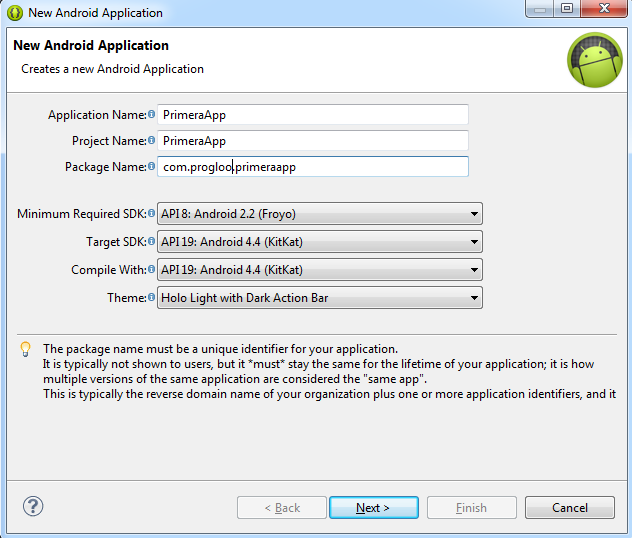
\includegraphics{asistente1.png}
\caption{Datos iniciales de la aplicación Android}\end{figure}

En ella deberemos prestar atención a los siguientes elementos:
\begin{itemize}
\item {} 
\emph{Minimum required SDK} : es la versión de Android mínima que necesitará en su móvil/tablet quien desee instalar la aplicación. Si se tiene la tentación de poner la versión 1.0 se debe tener en cuenta que también se dispondrán de menos clases y métodos para construir la app. La versión 8 (Android 2.1) es un valor razonable a día de hoy.

\item {} 
\emph{Target SDK} : es la versión de Android para la cual hemos optimizado la aplicación. En todo este manual se usará la versión 19 de Android (o Android 4.4)

\item {} 
\emph{Compile with} : Android tiene varias versiones y podemos utilizar una versión posterior para optimizar una aplicación orientada a un Android más antiguo. Sin embargo, normalmente no lo haremos y usaremos la misma versión que en el Target SDK, es decir, la 19.

\item {} 
\emph{Theme} : las aplicaciones pueden tener diversos temas o ``skins''. Google ofrece algunos estilos predeterminados, pero no haremos especial hincapie en el diseño, solo en la programación. Usaremos el estilo por defecto ``Holo Light''.

\end{itemize}

Despues de haber rellenado estos datos podremos ver algo como esto:
\begin{figure}[htbp]
\centering
\capstart

\scalebox{0.500000}{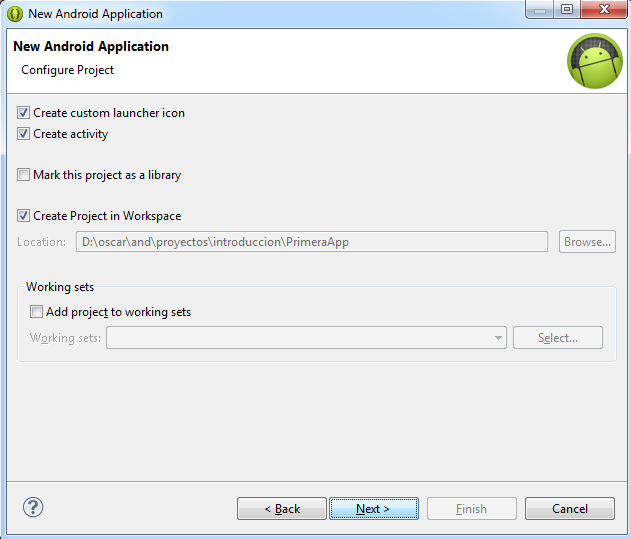
\includegraphics{asistente2.png}}
\caption{Opciones específicas del proyecto}{\small 
Aquí podremos indicar si queremos crear una biblioteca en lugar de una aplicación, si deseamos que se cree una actividad en blanco y si queremos ponerlo en el directorio de trabajo predeterminado. Se dejarán las opciones por defecto.
}\end{figure}
\begin{figure}[htbp]
\centering
\capstart

\scalebox{0.500000}{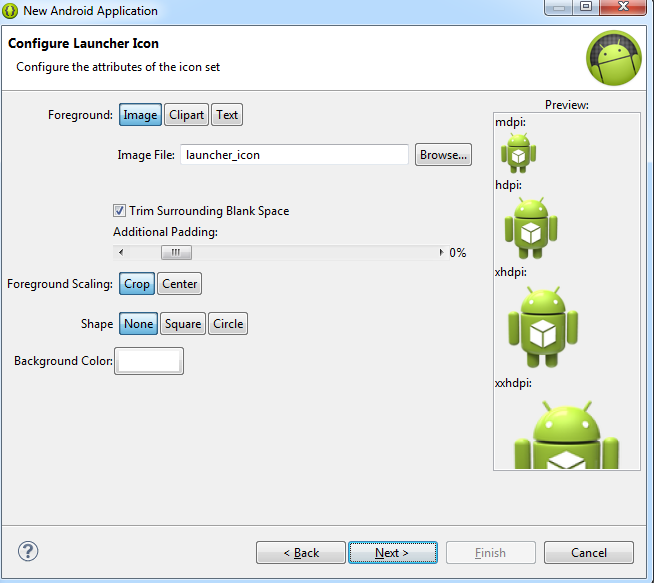
\includegraphics{asistente3.png}}
\caption{Personalizando el icono}{\small 
Esta ventana permite elegir algunas opciones sobre el icono de la aplicación:
}\end{figure}
\begin{figure}[htbp]
\centering
\capstart

\scalebox{0.500000}{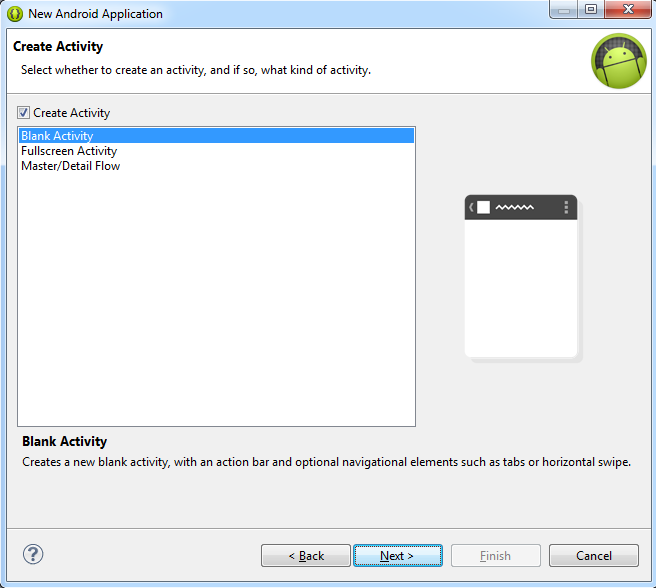
\includegraphics{asistente4.png}}
\caption{Tipo de actividad}{\small 
Aquí se puede elegir qué tipo de actividad se desea. En general, usaremos una actividad en blanco.
}\end{figure}
\begin{figure}[htbp]
\centering
\capstart

\scalebox{0.500000}{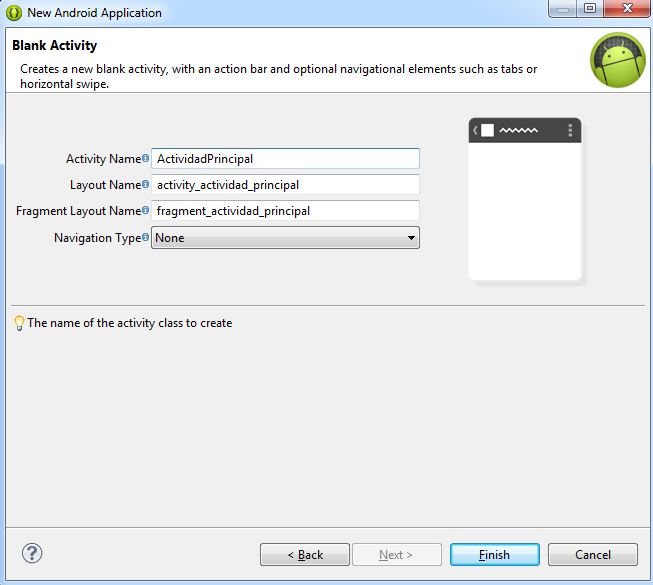
\includegraphics{asistente5.png}}
\caption{Datos de la actividad}{\small 
En este último paso se indicará el nombre de la clase que contendrá la actividad principal de la aplicación. Usaremos el nombre \code{ActividadPrincipal} y terminaremos el asistente.
}\end{figure}
\begin{figure}[htbp]
\centering
\capstart

\scalebox{0.500000}{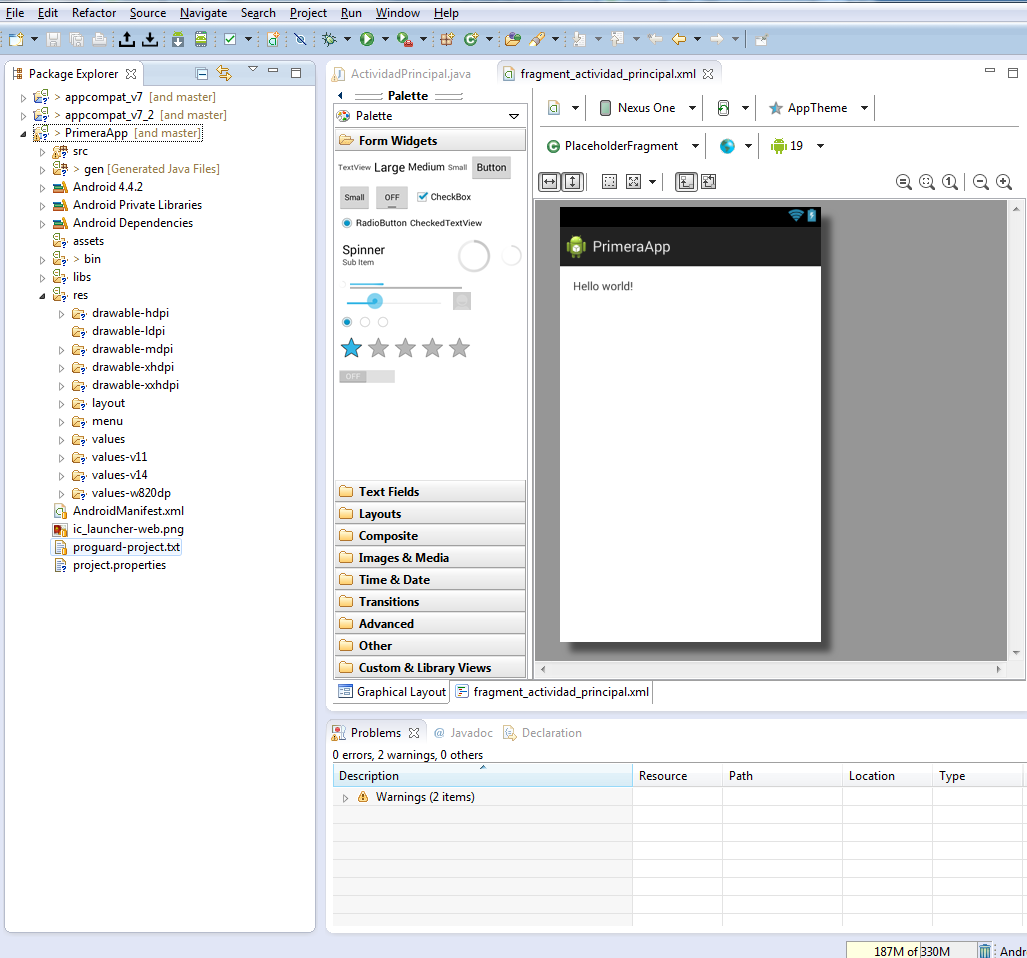
\includegraphics{proyectovacio.png}}
\caption{Un proyecto vacío de Android}{\small 
El asistente terminará y se nos mostrará el entorno de Eclipse.
}\end{figure}


\section{Descargando plataformas}
\label{tema1:descargando-plataformas}
Una vez hecho esto se debería instalar alguna versión del kit de desarrollo Android para empezar a programar. Para ello, se debe arrancar el gestor de plataformas Android mediante el menú de Eclipse \code{Window-\textgreater{}SDK Manager}
\begin{figure}[htbp]
\centering
\capstart

\scalebox{0.500000}{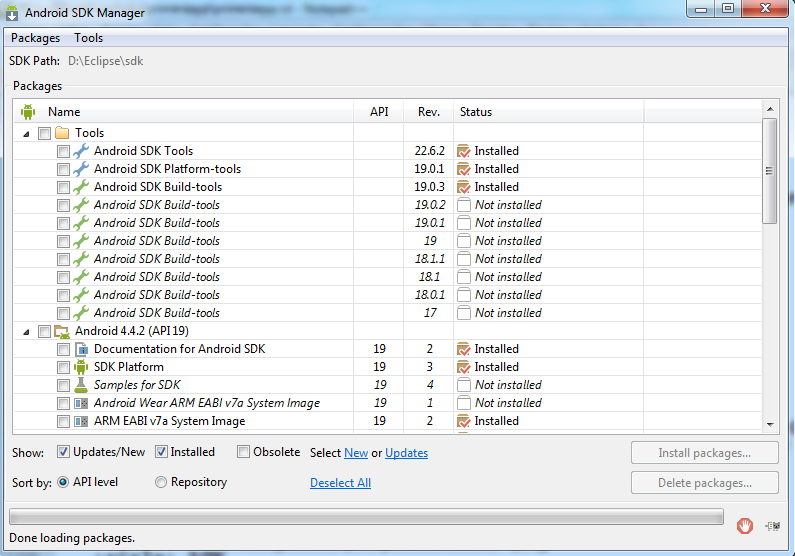
\includegraphics{sdkmanager.png}}
\caption{Administrador de plataformas Android}\end{figure}

El SDK Manager hace unas cuantas recomendaciones bastante prácticas: normalmente intentará instalar la última versión de Android más algunas herramientas útiles.

\begin{notice}{warning}{Advertencia:}
Una de las herramientas que se descargará es \emph{Intel x86 Emulator Accelerator} o HAXM. \href{http://software.intel.com/en-us/android/articles/intel-hardware-accelerated-execution-manager}{Esta herramienta de Intel} permite acelerar la ejecución del emulador de Android en microprocesadores Intel que tengan activada en su BIOS la opción de aceleración. Puede ser necesario habilitar esta opción en la BIOS (probablemente en alguna opción con el nombre \code{Enable Intel VT-x} o similar). El uso de HAXM es \textbf{MUY RECOMENDABLE}. Por otro lado, el SDK Manager descarga, pero no descomprime ni instala HAXM. Se debe buscar el ZIP en el directorio de instalación y ejecutarlo.
\end{notice}

En líneas generales se necesitarán:
\begin{itemize}
\item {} 
Todos los archivos de la última plataforma

\item {} 
El driver USB, que permitirá ejecutar nuestros programas en un móvil/tablet conectado por USB al equipo

\item {} 
El driver HAXM

\item {} 
La biblioteca de soporte de Android: permite que programas con una versión moderna se ejecuten en algunas plataformas más antiguas, entre otras cosas.

\item {} 
Las \emph{build-tools} o herramientas de compilación.

\item {} 
Las \emph{platform-tools} o herramientas específicas de la plataforma.

\item {} 
Las \emph{Android tools}, herramientas específicas de Android

\end{itemize}


\section{Creando emuladores}
\label{tema1:creando-emuladores}
Cuando se haya completado el paso anterior, se podrán crear \emph{Android Virtual Devices} o AVDs o emuladores. Se pueden crear dispositivos con diferentes características como se muestra a continuación.

En primer lugar, se debe elegir la opción \code{Window-Android Virtual Device Manager}, con lo que ser verá una herramienta que permite crear emuladores.
\begin{figure}[htbp]
\centering
\capstart

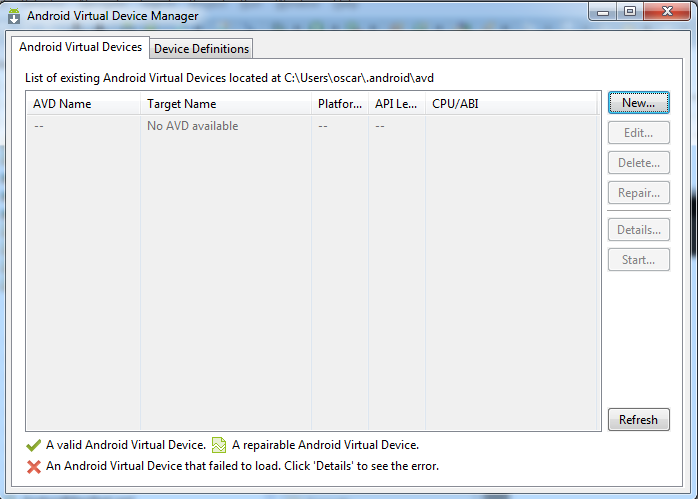
\includegraphics{avdmanager.png}
\caption{El Android Virtual Device Manager}\end{figure}
\begin{figure}[htbp]
\centering
\capstart

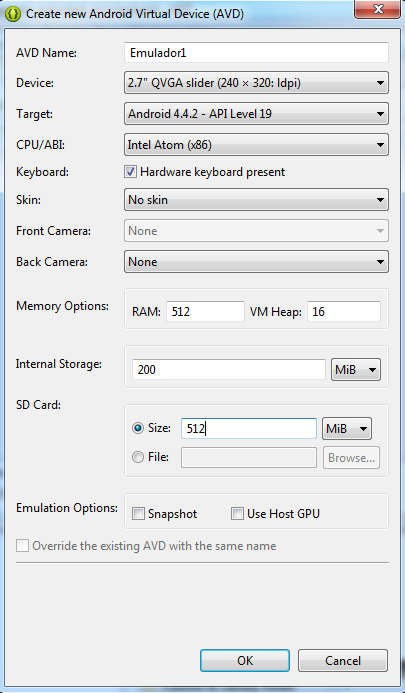
\includegraphics{creandoavd.png}
\caption{Creando dispositivos}{\small 
Una vez arrancado se podrá crear un nuevo dispositivo con el botón \emph{New}. Se recomienda mantener estas opciones.
}\end{figure}


\section{Arrancando el programa}
\label{tema1:arrancando-el-programa}
Una vez que se tiene el emulador creado, se puede arrancar con el botón Start, y despues arrancar el proyecto vacío Android de Eclipse. Para ello, una posibilidad es hacer click con el botón derecho en el proyecto que vemos a la izquierda de Eclipse y elegir el menu \code{Run As-Android Application}. Debería arrancarse la aplicación en el emulador y ver el resultado.
\begin{figure}[htbp]
\centering
\capstart

\scalebox{0.500000}{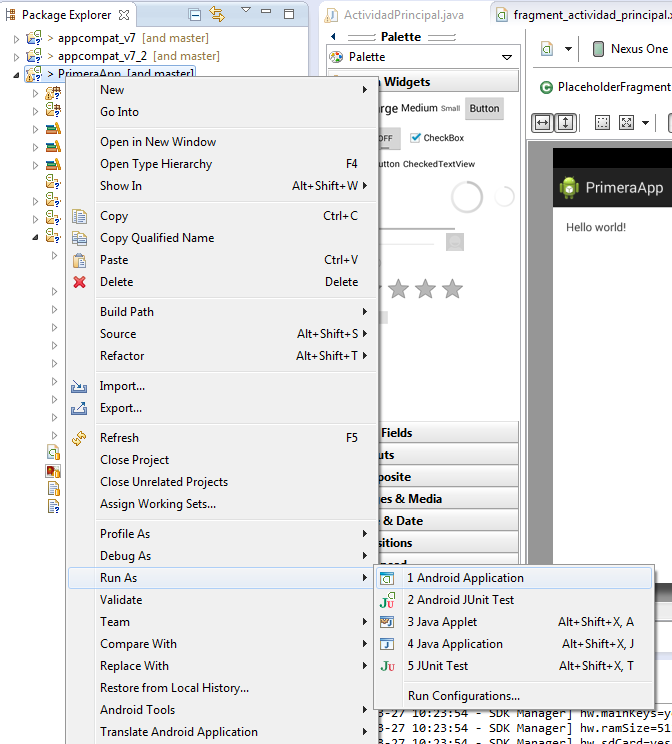
\includegraphics{ejecutandovacio.png}}
\caption{Ejecutando el primer proyecto}\end{figure}
\begin{figure}[htbp]
\centering
\capstart

\scalebox{0.500000}{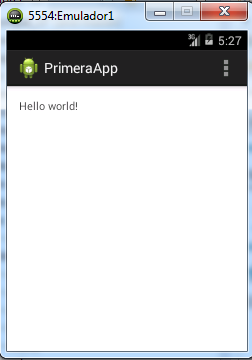
\includegraphics{primeraapp.png}}
\caption{Emulador ejecutando la primera app}\end{figure}


\section{Módulos para el desarrollo de aplicaciones móviles.}
\label{tema1:modulos-para-el-desarrollo-de-aplicaciones-moviles}
En este curso, realmente solo necesitaremos Java para crear apps. Sin embargo, existen un montón de bibliotecas que permiten acelerar el desarrollo para diversos lenguajes y distintas tareas. Solo por nombrar algunos mencionaremos:
\begin{itemize}
\item {} 
Unity para desarrollar juegos.

\item {} 
JQuery para Javascript.

\item {} 
Bibliotecas para tareas muy específicas como la seguridad SSL y similares.

\end{itemize}


\section{Emuladores.}
\label{tema1:emuladores}
A la hora de probar un app suele ser posible utilizar un emulador cargado en el sistema operativo que facilite la tarea de depurar la aplicación.

En Android, Google proporciona un sistema completo de emulación basado en máquinas virtuales (no usa VirtualBox sino un programa similar llamado QEMU).

El sistema de emulación permite crear dispositivos de características muy variadas para probar nuestra app en distintos entornos. Google denomina a estos dispositivos Android Virtual Devices (o AVDs)
\begin{itemize}
\item {} 
Se puede modificar el tamaño y la resolución.

\item {} 
La memoria RAM y espacio en tarjeta SD.

\item {} 
Se puede poner o quitar cámara.

\item {} 
Existen dispositivos predefinidos por Google que permiten crear emuladores muy rápidamente.

\item {} 
También se pueden clonar dispositivos para hacer solo una modificación de forma rápida.

\item {} 
Una característica de interés es que \emph{si se dispone de una tarjeta gráfica con aceleración} se puede activar una casilla llamada ``Host GPU'' que permite acelerar la emulación.

\item {} 
Se puede obligar al emulador a que ``recuerde'' el estado en que se quedó para así continuar donde nos hubiésemos quedado el último día. Esta opción se llama instantánea o \emph{snapshot}.

\end{itemize}

Si el equipo de escritorio es un Intel se puede instalar el Hardware Accelerated eXecution Manager o HAXM que permite acelerar la emulación. En el directorio \code{sdk/extras/intel} se puede encontrar un archivo ZIP que contiene un EXE que instala el HAXM. Se recomienda encarecidamente instalarlo en casa y, si es necesario, habilitar la tecnología VT en la BIOS.


\section{Ciclo de vida}
\label{tema1:ciclo-de-vida}\begin{figure}[htbp]
\centering
\capstart

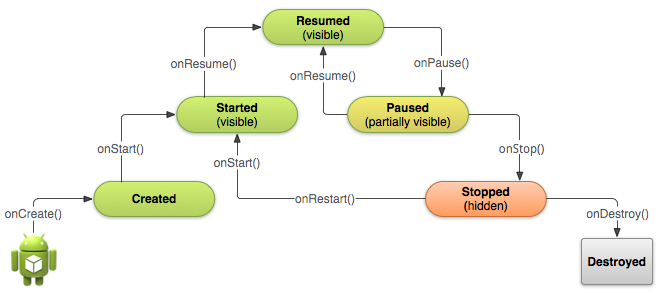
\includegraphics{ciclodevida.png}
\caption{Pasos en la ejecución de una app (imagen tomada de Google).}\end{figure}


\section{Configuraciones y perfiles}
\label{tema1:configuraciones-y-perfiles}

\section{Tamaños y densidades}
\label{tema1:tamanos-y-densidades}
Como ya se ha mencionado, la plataforma Android establece diversas categorías de dispositivo en función del tamaño y la densidad/resolución:
\begin{itemize}
\item {} 
En tamaños se distingue entre \emph{small} , \emph{normal}, \emph{large} y \emph{xlarge}.

\item {} 
En densidades se distingue entre \emph{ldpi}, \emph{mdpi}, \emph{hdpi} y \emph{xhdpi}.

\end{itemize}

\begin{notice}{tip}{Truco:}
Un cambio en la orientación del dispositivo \textbf{también se considera un cambio en el tamaño del dispositivo}.
\end{notice}
\begin{figure}[htbp]
\centering
\capstart

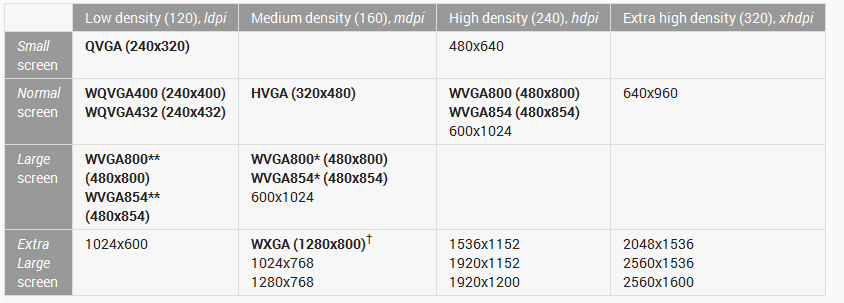
\includegraphics{tamaniospantalla.png}
\caption{Tamaños de pantalla (imagen tomada de Google)}\end{figure}


\section{Directorios}
\label{tema1:directorios}
Para que nuestra aplicación ofrezca soporte a todas estas variantes tan solo se deben utilizar distintos directorios \code{layout} dentro del subdirectorio \code{res}. Así, si queremos crear una configuración de interfaz diferente para pantallas grandes podemos crear un subdirectorio \code{res/layout-large} que contenga un interfaz diferente optimizada para pantallas grandes.

Como puede verse, la clave consiste en utilizar directorios \code{layout-xxx} donde \emph{xxx} pueden ser una serie de sufijos.
\begin{itemize}
\item {} 
\code{res/layout} es el directorio que se usará para el interfaz por defecto que asume orientación vertical.

\item {} 
\code{res/layout-large} para pantallas grandes.

\item {} 
\code{res/layout-xlarge} para pantallas muy grandes.

\item {} 
\code{res/layout-large-land} para pantallas muy grandes giradas para estar en horizontal (landscape).

\end{itemize}


\section{Imágenes}
\label{tema1:imagenes}
Cuando se tiene la previsión de que la aplicación se va a ejecutar en muchos dispositivos diferentes se deben crear diferentes versiones de las imágenes usadas.

Lo ideal es disponer de las imágenes en formato vectorial y utilizar las siguientes escalas:
\begin{itemize}
\item {} 
Para resoluciones \emph{mdpi}, la imagen a escala 1.

\item {} 
Para \emph{ldpi}, la imagen a escala 0.75

\item {} 
Para \emph{hdpi}, se escala a 1.5

\item {} 
Para \emph{xhdpi}, la escala debe ser 2.

\item {} 
Y así sucesivamente.

\end{itemize}

Normalmente ya no es necesario poner nada para \emph{ldpi} por dos motivos.
\begin{enumerate}
\item {} 
En la actualidad suponen un porcentaje muy pequeño de los dispositivos.

\item {} 
Android puede hacer la escala automáticamente.

\end{enumerate}

Aunque en este manual se habla en general de Android 4 conviene no perder de vista las plataformas anteriores. Google mantiene una pequeña tabla con \href{http://developer.android.com/about/dashboards/index.html}{los porcentajes de uso de las diversas versiones de Android} ya que crear nuestra aplicación \emph{exclusivamente para cierta versión y las posteriores} hará que nos autoexcluyamos de una porción del mercado que puede ser muy significativa.
\begin{figure}[htbp]
\centering
\capstart

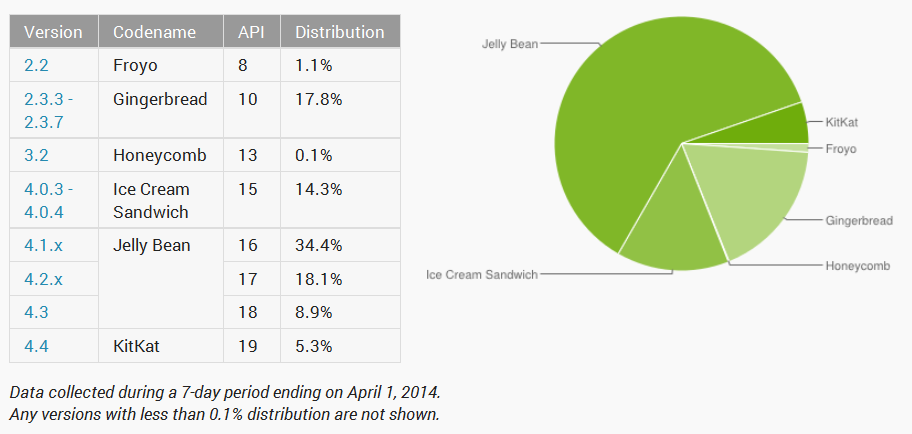
\includegraphics{porcentajesuso.png}
\caption{Porcentajes de uso de Android (tomada de Google el 4-4-2014)}\end{figure}


\section{Ejercicios}
\label{tema1:ejercicios}\begin{enumerate}
\item {} 
Crea una aplicación que se vea de tres formas distintas en función de que la pantalla sea normal, grande o muy grande

\item {} 
Haz que la aplicación anterior muestre datos sobre la plataforma sobre la que se está ejecutando. (Pista, deberás implementar \emph{forzosamente} un método \code{protected void onStart()})

\end{enumerate}

Para resolver estos ejercicios necesitarás leer los apartados siguientes sobre directorios y recursos.


\section{Solución Ejercicio 1}
\label{tema1:solucion-ejercicio-1}

\subsection{Enunciado}
\label{tema1:enunciado}
\emph{Crea una aplicación que se vea de tres formas distintas en función de que la pantalla sea normal, grande o muy grande} .

Para poder ver los resultados deberemos tener en primer lugar tres emuladores, que tengan, los tamaños que necesitamos.
\begin{figure}[htbp]
\centering
\capstart

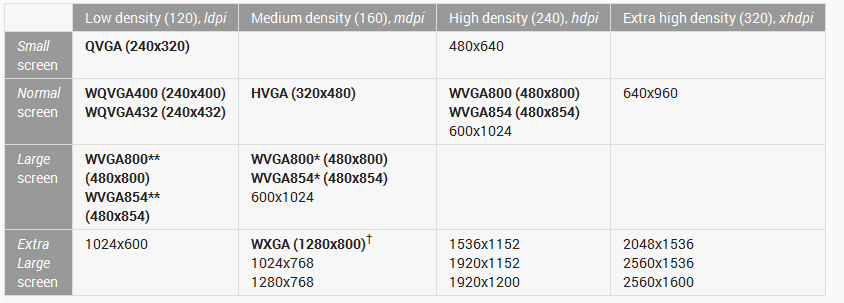
\includegraphics{tamaniospantalla.png}
\caption{Tamaños de pantalla reconocidos (imagen tomada de Google)}\end{figure}


\subsection{Implementación}
\label{tema1:implementacion}
Una vez creados los AVDs crearemos el proyecto, en el cual Eclipse nos creará automáticamente el directorio \code{res/layout}. Crearemos dos directorios más:
\begin{enumerate}
\item {} 
\code{res/layout-large} donde pondremos los ficheros con la interfaz definido para pantallas grandes.

\item {} 
\code{res/layout-xlarge} para pantallas muy grandes. Si no se tiene memoria suficiente es posible que un emulador con estas características tarde mucho en arrancar e incluso que sufra ``cuelgues''.

\end{enumerate}

Crearemos un interfaz cualquiera como por ejemplo este:

\begin{Verbatim}[commandchars=\\\{\}]
\PYG{n+nt}{\PYGZlt{}RelativeLayout} \PYG{n+na}{xmlns:android=}\PYG{l+s}{\PYGZdq{}http://schemas.android.com/apk/res/android\PYGZdq{}}
        \PYG{n+na}{xmlns:tools=}\PYG{l+s}{\PYGZdq{}http://schemas.android.com/tools\PYGZdq{}}
        \PYG{n+na}{android:layout\PYGZus{}width=}\PYG{l+s}{\PYGZdq{}match\PYGZus{}parent\PYGZdq{}}
        \PYG{n+na}{android:layout\PYGZus{}height=}\PYG{l+s}{\PYGZdq{}match\PYGZus{}parent\PYGZdq{}}
        \PYG{n+na}{android:paddingBottom=}\PYG{l+s}{\PYGZdq{}@dimen/activity\PYGZus{}vertical\PYGZus{}margin\PYGZdq{}}
        \PYG{n+na}{android:paddingLeft=}\PYG{l+s}{\PYGZdq{}@dimen/activity\PYGZus{}horizontal\PYGZus{}margin\PYGZdq{}}
        \PYG{n+na}{android:paddingRight=}\PYG{l+s}{\PYGZdq{}@dimen/activity\PYGZus{}horizontal\PYGZus{}margin\PYGZdq{}}
        \PYG{n+na}{android:paddingTop=}\PYG{l+s}{\PYGZdq{}@dimen/activity\PYGZus{}vertical\PYGZus{}margin\PYGZdq{}}
        \PYG{n+na}{tools:context=}\PYG{l+s}{\PYGZdq{}com.example.adapptable.ActividadPrincipal\PYGZdl{}PlaceholderFragment\PYGZdq{}} \PYG{n+nt}{\PYGZgt{}}

        \PYG{n+nt}{\PYGZlt{}TextView}
                \PYG{n+na}{android:id=}\PYG{l+s}{\PYGZdq{}@+id/textView1\PYGZdq{}}
                \PYG{n+na}{android:layout\PYGZus{}width=}\PYG{l+s}{\PYGZdq{}wrap\PYGZus{}content\PYGZdq{}}
                \PYG{n+na}{android:layout\PYGZus{}height=}\PYG{l+s}{\PYGZdq{}wrap\PYGZus{}content\PYGZdq{}}
                \PYG{n+na}{android:layout\PYGZus{}alignParentBottom=}\PYG{l+s}{\PYGZdq{}true\PYGZdq{}}
                \PYG{n+na}{android:layout\PYGZus{}alignParentRight=}\PYG{l+s}{\PYGZdq{}true\PYGZdq{}}
                \PYG{n+na}{android:text=}\PYG{l+s}{\PYGZdq{}@string/textoPlataformas\PYGZdq{}} \PYG{n+nt}{/\PYGZgt{}}

\PYG{n+nt}{\PYGZlt{}/RelativeLayout\PYGZgt{}}
\end{Verbatim}

Como se puede apreciar, solo contiene un cuadro de texto que debe aparecer \textbf{en la esquina inferior derecha} del dispositivo.

Una vez hecho esto, pondremos en los otros directorios alguna variación de este fichero, como por ejemplo estas dos:

\begin{Verbatim}[commandchars=\\\{\}]
\PYG{n+nt}{\PYGZlt{}RelativeLayout} \PYG{n+na}{xmlns:android=}
\PYG{l+s}{\PYGZdq{}http://schemas.android.com/apk/res/android\PYGZdq{}}
        \PYG{n+na}{xmlns:tools=}\PYG{l+s}{\PYGZdq{}http://schemas.android.com/tools\PYGZdq{}}
        \PYG{n+na}{android:layout\PYGZus{}width=}\PYG{l+s}{\PYGZdq{}match\PYGZus{}parent\PYGZdq{}}
        \PYG{n+na}{android:layout\PYGZus{}height=}\PYG{l+s}{\PYGZdq{}match\PYGZus{}parent\PYGZdq{}}
        \PYG{n+na}{android:paddingBottom=}\PYG{l+s}{\PYGZdq{}@dimen/activity\PYGZus{}vertical\PYGZus{}margin\PYGZdq{}}
        \PYG{n+na}{android:paddingLeft=}\PYG{l+s}{\PYGZdq{}@dimen/activity\PYGZus{}horizontal\PYGZus{}margin\PYGZdq{}}
        \PYG{n+na}{android:paddingRight=}\PYG{l+s}{\PYGZdq{}@dimen/activity\PYGZus{}horizontal\PYGZus{}margin\PYGZdq{}}
        \PYG{n+na}{android:paddingTop=}\PYG{l+s}{\PYGZdq{}@dimen/activity\PYGZus{}vertical\PYGZus{}margin\PYGZdq{}}
        \PYG{n+na}{tools:context=}
        \PYG{l+s}{\PYGZdq{}com.example.adapptable.ActividadPrincipal\PYGZdl{}PlaceholderFragment\PYGZdq{}} \PYG{n+nt}{\PYGZgt{}}

        \PYG{n+nt}{\PYGZlt{}TextView}
                \PYG{n+na}{android:id=}\PYG{l+s}{\PYGZdq{}@+id/textView1\PYGZdq{}}
                \PYG{n+na}{android:layout\PYGZus{}width=}\PYG{l+s}{\PYGZdq{}wrap\PYGZus{}content\PYGZdq{}}
                \PYG{n+na}{android:layout\PYGZus{}height=}\PYG{l+s}{\PYGZdq{}wrap\PYGZus{}content\PYGZdq{}}
                \PYG{n+na}{android:layout\PYGZus{}centerHorizontal=}\PYG{l+s}{\PYGZdq{}true\PYGZdq{}}
                \PYG{n+na}{android:layout\PYGZus{}centerVertical=}\PYG{l+s}{\PYGZdq{}true\PYGZdq{}}
                \PYG{n+na}{android:text=}\PYG{l+s}{\PYGZdq{}@string/textoPlataformas\PYGZdq{}} \PYG{n+nt}{/\PYGZgt{}}
        \PYG{c}{\PYGZlt{}!\PYGZhy{}\PYGZhy{}}\PYG{c}{El cuadro debe aparecer}
\PYG{c}{        en el centro de la pantalla}\PYG{c}{\PYGZhy{}\PYGZhy{}\PYGZgt{}}

\PYG{n+nt}{\PYGZlt{}/RelativeLayout\PYGZgt{}}
\end{Verbatim}

\begin{Verbatim}[commandchars=\\\{\}]
\PYG{n+nt}{\PYGZlt{}RelativeLayout} \PYG{n+na}{xmlns:android=}
        \PYG{l+s}{\PYGZdq{}http://schemas.android.com/apk/res/android\PYGZdq{}}
        \PYG{n+na}{xmlns:tools=}\PYG{l+s}{\PYGZdq{}http://schemas.android.com/tools\PYGZdq{}}
        \PYG{n+na}{android:layout\PYGZus{}width=}\PYG{l+s}{\PYGZdq{}match\PYGZus{}parent\PYGZdq{}}
        \PYG{n+na}{android:layout\PYGZus{}height=}\PYG{l+s}{\PYGZdq{}match\PYGZus{}parent\PYGZdq{}}
        \PYG{n+na}{android:paddingBottom=}\PYG{l+s}{\PYGZdq{}@dimen/activity\PYGZus{}vertical\PYGZus{}margin\PYGZdq{}}
        \PYG{n+na}{android:paddingLeft=}\PYG{l+s}{\PYGZdq{}@dimen/activity\PYGZus{}horizontal\PYGZus{}margin\PYGZdq{}}
        \PYG{n+na}{android:paddingRight=}\PYG{l+s}{\PYGZdq{}@dimen/activity\PYGZus{}horizontal\PYGZus{}margin\PYGZdq{}}
        \PYG{n+na}{android:paddingTop=}\PYG{l+s}{\PYGZdq{}@dimen/activity\PYGZus{}vertical\PYGZus{}margin\PYGZdq{}}
        \PYG{n+na}{tools:context=}
        \PYG{l+s}{\PYGZdq{}com.example.adapptable.ActividadPrincipal\PYGZdl{}PlaceholderFragment\PYGZdq{}} \PYG{n+nt}{\PYGZgt{}}

        \PYG{n+nt}{\PYGZlt{}TextView}
                \PYG{n+na}{android:id=}\PYG{l+s}{\PYGZdq{}@+id/textView1\PYGZdq{}}
                \PYG{n+na}{android:layout\PYGZus{}width=}\PYG{l+s}{\PYGZdq{}wrap\PYGZus{}content\PYGZdq{}}
                \PYG{n+na}{android:layout\PYGZus{}height=}\PYG{l+s}{\PYGZdq{}wrap\PYGZus{}content\PYGZdq{}}
                \PYG{n+na}{android:layout\PYGZus{}alignParentTop=}\PYG{l+s}{\PYGZdq{}true\PYGZdq{}}
                \PYG{n+na}{android:layout\PYGZus{}centerHorizontal=}\PYG{l+s}{\PYGZdq{}true\PYGZdq{}}
                \PYG{n+na}{android:text=}\PYG{l+s}{\PYGZdq{}@string/textoPlataformas\PYGZdq{}} \PYG{n+nt}{/\PYGZgt{}}
        \PYG{c}{\PYGZlt{}!\PYGZhy{}\PYGZhy{}}\PYG{c}{El cuadro debe aparecer}
\PYG{c}{        centrado en la parte superior}\PYG{c}{\PYGZhy{}\PYGZhy{}\PYGZgt{}}
\PYG{n+nt}{\PYGZlt{}/RelativeLayout\PYGZgt{}}
\end{Verbatim}
\begin{figure}[htbp]
\centering
\capstart

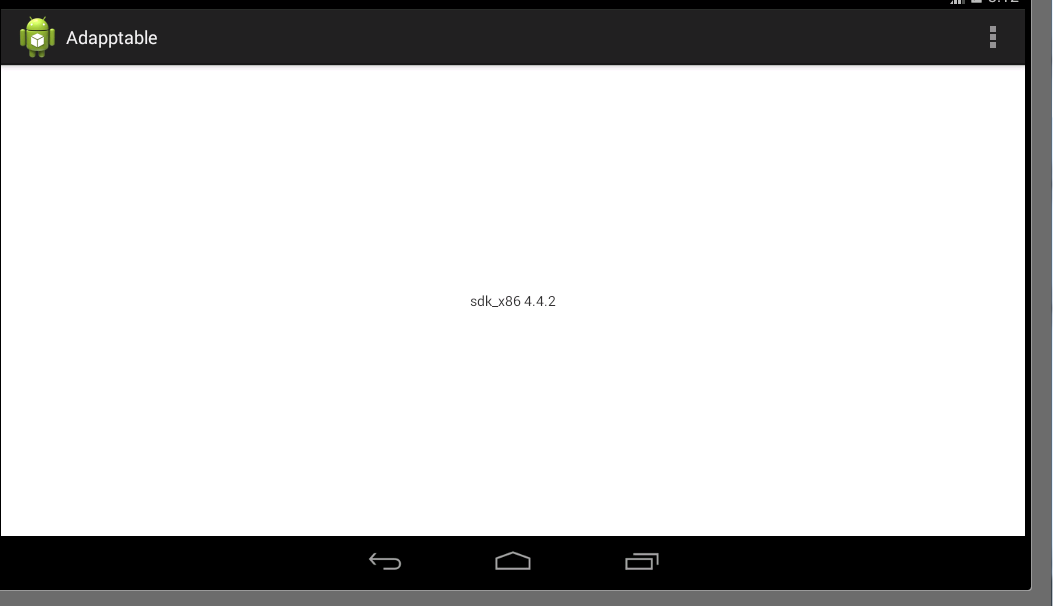
\includegraphics{distintostamanios.png}
\caption{Vista de la aplicación en una tablet.}\end{figure}
\begin{figure}[htbp]
\centering
\capstart

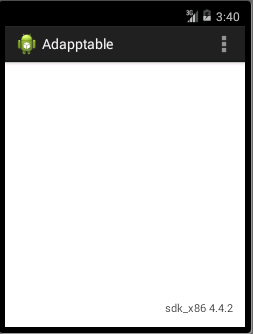
\includegraphics{distintostamanios2.png}
\caption{Vista de la aplicación en un móvil.}\end{figure}


\section{Directorios}
\label{tema1:id1}
Como ya se ha introducido anteriormente ciertos elementos que pueden cambiar no deberían estar dentro del código, sino en \emph{recursos} (es decir, en ficheros externos que puedan cargarse en tiempo de ejecución). Un ejemplo muy elemental son las cadenas: si queremos ofrecer soporte a varios idiomas, es mejor tener todas las cadenas en un fichero, de forma que si queremos traducir la aplicación, bastará con traducir dicho fichero y hacer que la aplicación cargue distintos ficheros en función el idioma.
\begin{figure}[htbp]
\centering
\capstart

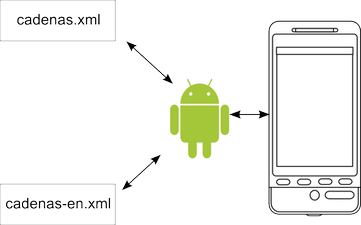
\includegraphics{cadenasmultiples.png}
\caption{Un mismo código fuente, distintas cadenas (Imagen de \href{http://openclipart.org/user-detail/shokunin}{shokunin} ).}\end{figure}

Veamos un ejemplo muy simple. Supongamos que la aplicación saluda al usuario en el momento del arranque. Podríamos usar este código Java.

\begin{Verbatim}[commandchars=\\\{\}]
\PYG{k+kd}{public} \PYG{k+kd}{class} \PYG{n+nc}{Actividad}\PYG{o}{\PYGZob{}}
        \PYG{k+kd}{private} \PYG{k+kd}{final} \PYG{n}{String} \PYG{n}{saludo}\PYG{o}{=}\PYG{l+s}{\PYGZdq{}Hola\PYGZdq{}}\PYG{o}{;}
\PYG{o}{\PYGZcb{}}
\end{Verbatim}

Sin embargo, al hacerlo así, la traducción de la aplicación se vuelve muy compleja. Sin embargo, podemos almacenar las cadenas en un fichero de recursos como \code{strings.xml} de esta forma.

\begin{Verbatim}[commandchars=\\\{\}]
\PYG{n+nt}{\PYGZlt{}string} \PYG{n+na}{id=}\PYG{l+s}{\PYGZdq{}saludo\PYGZdq{}}\PYG{n+nt}{\PYGZgt{}}Hola\PYG{n+nt}{\PYGZlt{}/string\PYGZgt{}}
\end{Verbatim}

Si ahora en el código Java cargamos la cadena (en pseudocódigo)...

\begin{Verbatim}[commandchars=\\\{\}]
\PYG{k+kd}{public} \PYG{k+kt}{void} \PYG{n+nf}{saludar}\PYG{o}{(}\PYG{o}{)}\PYG{o}{\PYGZob{}}
        \PYG{n}{String} \PYG{n}{saludo}\PYG{o}{=}\PYG{n}{R}\PYG{o}{.}\PYG{n+na}{string}\PYG{o}{.}\PYG{n+na}{saludo}\PYG{o}{;}
\PYG{o}{\PYGZcb{}}
\end{Verbatim}

...ahora la traducción es muy sencilla, ya que basta con tener otro fichero en la aplicación con las cadenas en inglés:

\begin{Verbatim}[commandchars=\\\{\}]
\PYG{n+nt}{\PYGZlt{}string} \PYG{n+na}{id=}\PYG{l+s}{\PYGZdq{}saludo\PYGZdq{}}\PYG{n+nt}{\PYGZgt{}}Hello\PYG{n+nt}{\PYGZlt{}/string\PYGZgt{}}
\end{Verbatim}

\emph{Y no habrá que tocar nada del código Java}. De hecho, Android compilar los recursos para que sean fácilmente accesibles desde código Java. En este capítulo se analiza como usar los recursos.


\section{Tipos de recursos}
\label{tema1:tipos-de-recursos}
Todos los recursos se definen en forma de XML y \emph{deben} ir dentro de uno de estos subdirectorios que hay dentro de \code{res}:
\begin{itemize}
\item {} 
\code{res/animator}: contiene los ficheros XML que especifican animaciones. Se verá más sobre animaciones más adelante.

\item {} 
\code{res/anim}: aquí se pondrán unos tipos especiales de animación llamadas ``tween animation'' que permiten a Android generar la animación a partir de información tal como ``punto inicial'', ``punto final'' y ``duración de la animación''.

\item {} 
\code{res/color}: define los colores de nuestra aplicación.

\item {} 
\code{res/drawable}: para especificar los archivos de imagen usados (en formatos .png, .9.png, .jpg y .gif)

\item {} 
\code{res/layout}: para indicar la colocación de recursos en pantalla en los distintos tamaños de pantalla.

\item {} 
\code{res/menu}: define los menús de aplicación.

\item {} 
\code{res/raw}: recursos almacenados en formato binario. Pueden cargarse con \code{Resources.openRawResource()}

\item {} 
\code{res/values}: ficheros XML que contienen valores simples como números, cadenas o incluso colores. Aunque en realidad aquí se pueden usar los nombres de fichero que queramos la costumbre es usar estos nombres:
\begin{itemize}
\item {} 
arrays.xml: permite crear vectores de recursos.

\item {} 
colors.xml: para colores.

\item {} 
dimens.xml: para especificar tamaños.

\item {} 
strings.xml: para cadenas.

\item {} 
styles.xml: para estilos

\end{itemize}

\item {} 
\code{res/xml}: aquí se almacena cualquier otro fichero XML que se desee. Los ficheros en este directorio pueden cargarse usando \code{Resources.getXML()}

\end{itemize}

Existe una última posibilidad para almacenar recursos, que es usar el directorio \code{assets} (no es \code{res/assets}) sin embargo, Android no compila dichos recursos automáticamente. Deben cargarse con la clase AssetsManager.


\section{Indicando recursos alternativos}
\label{tema1:indicando-recursos-alternativos}
Por ejemplo, ya sabemos que el archivo \code{res/values/strings.xml} contiene las cadenas que se mostrarán por defecto. Si esas cadenas están en español y deseamos indicar que se carguen otras cadenas para el idioma inglés se deben indicar modificadores para el directorio \code{values}.
\begin{itemize}
\item {} 
\code{res/values-en/strings.xml} indicaría el fichero de cadenas para el idioma inglés.

\item {} 
\code{res/values-fr/strings.xml} para francés.

\item {} 
Se puede usar cualquier \href{http://www.loc.gov/standards/iso639-2/php/code\_list.php}{código ISO 639-1} para indicar el idioma.

\end{itemize}

Los modificadores se pueden añadir a cualquier subdirectorio de los vistos antes, además se pueden poner varios a la vez pero siempre respetando este orden:
\begin{enumerate}
\item {} 
MCC (Mobile Country Code o código de país) y MNC (Mobile Network Code o código de red). Pueden consultarse las distintas redes y países en \href{http://es.wikipedia.org/wiki/MCC/MNC}{Wikipedia} . Por ejemplo para indicar un recurso específico de un teléfono Android usado en territorio español se usaría \code{mcc214} y para indicar específicamente un recurso en un Android que accede desde Movistar se usaría \code{mcc214-mnc07}.

\item {} 
Idioma y región: se usa un código de páis ISO 639-1 que puede o no ir seguido de una ``r'' y un código de región. Así el modificador ``en'' indica idioma inglés y ``fr'' francés, pero ``fr-rFR'' indica francés de Francia y ``fr-rCA'' francés de Canadá. Pueden consultarse los códigos de país en \href{http://en.wikipedia.org/wiki/List\_of\_ISO\_639-1\_codes}{Wikipedia}

\item {} 
Dirección de lectura: \code{ldrtl} para cuando el idioma del dispositivo se lee de derecha a izquierda (right-to-left) y \code{ldltr} para lectura de izquierda a derecha. Obsérvese que ya podriamos indicar un fichero \code{res/values-mcc214-fr-rCA/strings.xml} para indicar los textos que debe usar un teléfono Android con su idioma puesto a francés (de Canadá) que sin embargo usa una red española. Sin embargo \code{res/values-fr-mcc214/strings.xml} estaría mal ya que aunque el idioma y el territorio son correctos los hemos puesto al revés (sería \code{res/values-mcc214-fr})

\item {} 
Anchura mínima del dispositivo: se usa \code{swNdp} donde N es el número mínimo de puntos que debe tener la anchura de la pantalla. También puede indicarse este valor en el \code{AndroidManifest.xml} con el atributo \code{android:requiresSmallestWidthDp}. Si indicamos varios directorios, Android escogerá siempre el valor de N más pequeño y cercano a la anchura del dispositivo \textbf{independientemente de si la pantalla se gira o no}. Algunos valores típicos son:
\begin{itemize}
\item {} 
sw320dp: para pantallas de 240x320 (ldpi), de 320x480 (mdpi) o de 480x800 (hdpi)

\item {} 
sw480dp: para 480x800 (mdpi)

\item {} 
sw600dp: para 600x1024 (mdpi)

\end{itemize}

\item {} 
Anchura disponible: el sufijo \code{wNdp} indica la anchura que la aplicación necesita \textbf{teniendo en cuenta si la pantalla se gira} (esta es la diferencia con respecto al anterior).

\item {} 
Altura disponible: el sufijo \code{hNdp} indica la altura que la aplicación necesita.

\item {} 
Tamaño de pantalla: pueden usarse los sufijos siguientes:
\begin{itemize}
\item {} 
\code{small} de aproximadamente 320x426

\item {} 
\code{normal} aproximadamente 320x470

\item {} 
\code{large} de unos 480x640

\item {} 
\code{xlarge} con un tamaño de 720x960 (normalmente tablets)

\end{itemize}

\item {} 
Aspecto de la pantalla: \code{long}     para pantallas WQVGA, WVGA, FWVGA y \code{notlong} para QVGA, HVGA, and VGA. No tiene nada que ver con la orientación de la pantalla.

\item {} 
Orientación de la pantalla: \code{port} (portrait) para cuando la pantalla está en vertical y \code{land} (landscape) para cuando está en horizontal.

\item {} 
Modo del interfaz de usuario:
\begin{itemize}
\item {} 
\code{car} cuando el dispositivo está en un coche.

\item {} 
\code{desk} en un escritorio

\item {} 
\code{television}

\item {} 
\code{appliance} el dispositivo es una herramienta y no tiene pantalla.

\end{itemize}

\item {} 
Modo nocturno: \code{night} y \code{notnight} dependiendo de si el dispositivo está en modo nocturno o no.

\item {} 
Densidad de pixeles: (la escala entre los principales tamaños es 3:4:6:8)
\begin{itemize}
\item {} 
ldpi: pantallas de baja densidad, aproximadamente 120dpi.

\item {} 
mdpi: densidad media, unos 160dpi.

\item {} 
hdpi: alta densidad, unos 240dpi.

\item {} 
xhdpi: densidad ``extra-alta'', unos 320dpi.

\item {} 
nodpi: Usado para recursos para los que no queremos que Android haga el escalado.

\item {} 
tvdpi: unos 213 (entre \code{mdpi} y \code{hdpi})

\end{itemize}

\item {} 
Tipo de pantalla: \code{finger} para dispositivos táctiles y \code{notouch} para los demás.

\item {} 
Disponibilidad de teclado:
\begin{itemize}
\item {} 
\code{keysexposed}: hay teclado hardware.

\item {} 
\code{keyshidden}: hay teclado hardware pero no está disponible y además \emph{no hay teclado software}.

\item {} 
\code{keyssoft}: hay teclado software.

\end{itemize}

\item {} 
Método de entrada: \code{nokeys} cuando no hay teclado hardware, \code{qwerty} si hay un teclado hardware y \code{12key} para teclados hardware de 12 teclas.

\item {} 
Disponibilidad de teclas de navegación:
\begin{itemize}
\item {} 
\code{nonav}: no se puede navegar con teclas.

\item {} 
\code{dpad}: hay un pad direccional.

\item {} 
\code{trackball}: hay un trackball.

\item {} 
\code{wheel}:  hay un ratón con rueda (poco habitual).

\end{itemize}

\item {} 
Versión de la plataforma Android: \code{v3}, \code{v4}, \code{v9} etc...

\end{enumerate}


\section{Ejercicio}
\label{tema1:ejercicio}
¿Como debería llamarse un directorio que contuviera recursos específicos para un teléfono en portugués que esté usándose en Francia con el operador Bouygues Telecom y que fuera un dispositivo de una resolución hdpi?

Respuesta: hay que ir nombrando el directorio con los sufijos correctos en el orden correcto. En este caso sería \code{values-mcc208-mnc20-pt-hdpi}.


\section{Tamaños y densidades}
\label{tema1:id3}
En la tabla siguiente, tomada de la documentación oficial de Google pueden verse los tamaños y densidades aproximados de los distintos tipos de pantalla que podemos encontrar.
\begin{figure}[htbp]
\centering
\capstart

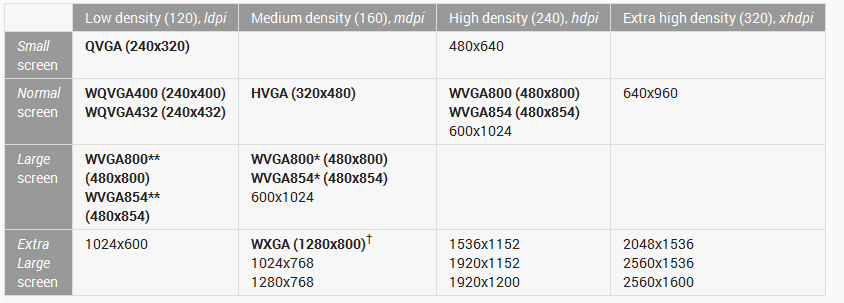
\includegraphics{tamaniospantalla.png}
\caption{Tamaños de pantalla reconocidos (imagen tomada de Google)}\end{figure}


\section{Accediendo a los recursos}
\label{tema1:accediendo-a-los-recursos}
Cuando se crea un recurso puede accederse al mismo por medio de la clase especial \code{R} la cual es creada por la herramienta \code{aapt}. Dicha herramienta toma todos los recursos y crea distintas subclases para facilitar el uso de dichos recursos. Las clases creadas son:
\begin{itemize}
\item {} 
R.drawable: para acceder a archivos de imagen.

\item {} 
R.id: para acceder al id de un control.

\item {} 
R.layout: para cargar disposiciones de controles.

\item {} 
R.string: para acceder a cadenas.

\end{itemize}

Aí, por ejemplo si un archivo de imagen ubicado en \code{res/drawable/icono.png} quiere ponerse de fondo en algún control se usará la sentencia:

\begin{Verbatim}[commandchars=\\\{\}]
\PYG{n}{control}\PYG{o}{.}\PYG{n+na}{setBackgroundDrawableResource}\PYG{o}{(}
        \PYG{n}{R}\PYG{o}{.}\PYG{n+na}{drawable}\PYG{o}{.}\PYG{n+na}{icono}\PYG{o}{)}\PYG{o}{;}
\end{Verbatim}

Por otro lado, si deseamos usar un recurso XML en otro archivo XML se puede hacer usando la siguiente estructura:
\begin{enumerate}
\item {} 
Empezar siempre por \code{@}

\item {} 
Si se desea acceder a un recurso en otro paquete poner el nombre seguido de \code{:}, como \code{com.ejemplo:}.

\item {} 
Despues se indica el tipo de recurso, \code{string}, \code{drawable}...

\item {} 
Despues se indica el nombre del recurso.

\end{enumerate}

Supongamos que tenemos un fichero genérico con distintas definiciones de recursos como este:

\begin{Verbatim}[commandchars=\\\{\}]
\PYG{c+cp}{\PYGZlt{}?xml version=\PYGZdq{}1.0\PYGZdq{} encoding=\PYGZdq{}utf\PYGZhy{}8\PYGZdq{}?\PYGZgt{}}
\PYG{n+nt}{\PYGZlt{}resources}\PYG{n+nt}{\PYGZgt{}}
   \PYG{n+nt}{\PYGZlt{}color} \PYG{n+na}{name=}\PYG{l+s}{\PYGZdq{}color\PYGZus{}corporativo\PYGZdq{}}\PYG{n+nt}{\PYGZgt{}}\PYGZsh{}f00\PYG{n+nt}{\PYGZlt{}/color\PYGZgt{}}
   \PYG{n+nt}{\PYGZlt{}string} \PYG{n+na}{name=}\PYG{l+s}{\PYGZdq{}saludo\PYGZdq{}}\PYG{n+nt}{\PYGZgt{}}Hola\PYG{n+nt}{\PYGZlt{}/string\PYGZgt{}}
\PYG{n+nt}{\PYGZlt{}/resources\PYGZgt{}}
\end{Verbatim}

Y que deseamos usar este color y este texto en interfaz. El XML sería así:

\begin{Verbatim}[commandchars=\\\{\}]
\PYG{c+cp}{\PYGZlt{}?xml version=\PYGZdq{}1.0\PYGZdq{} encoding=\PYGZdq{}utf\PYGZhy{}8\PYGZdq{}?\PYGZgt{}}
\PYG{n+nt}{\PYGZlt{}EditText}
        \PYG{n+na}{xmlns:android=}
          \PYG{l+s}{\PYGZdq{}http://schemas.android.com/apk/res/android\PYGZdq{}}
        \PYG{n+na}{android:layout\PYGZus{}width=}\PYG{l+s}{\PYGZdq{}fill\PYGZus{}parent\PYGZdq{}}
        \PYG{n+na}{android:layout\PYGZus{}height=}\PYG{l+s}{\PYGZdq{}fill\PYGZus{}parent\PYGZdq{}}
        \PYG{n+na}{android:textColor=}\PYG{l+s}{\PYGZdq{}@color/color\PYGZus{}corporativo\PYGZdq{}}
        \PYG{n+na}{android:text=}\PYG{l+s}{\PYGZdq{}@string/saludo\PYGZdq{}} \PYG{n+nt}{/\PYGZgt{}}
\end{Verbatim}

Por último mencionar que Android dispone de muchos otros recursos a los cuales se puede acceder usando el prefijo \code{android}. Así, por ejemplo, Android define un interfaz para elementos en una lista que podemos usar con este código (obsérvese que Android llama a este interfaz \code{simple\_list\_item\_1}):

\begin{Verbatim}[commandchars=\\\{\}]
\PYG{n}{setListAdapter}\PYG{o}{(}
        \PYG{k}{new} \PYG{n}{ArrayAdapter}\PYG{o}{\PYGZlt{}}\PYG{n}{String}\PYG{o}{\PYGZgt{}}\PYG{o}{(}
                \PYG{k}{this}\PYG{o}{,}
                \PYG{n}{android}\PYG{o}{.}\PYG{n+na}{R}\PYG{o}{.}\PYG{n+na}{layout}\PYG{o}{.}\PYG{n+na}{simple\PYGZus{}list\PYGZus{}item\PYGZus{}1}\PYG{o}{,}
                \PYG{n}{vector}
        \PYG{o}{)}
\PYG{o}{)}\PYG{o}{;}
\end{Verbatim}


\section{Gestión de cambios durante la ejecución}
\label{tema1:gestion-de-cambios-durante-la-ejecucion}
Android puede decidir reiniciar nuestra app por diversos motivos:
\begin{itemize}
\item {} 
El usuario ha cambiado el idioma.

\item {} 
La pantalla ha rotado por ejemplo de vertical a horizontal.

\item {} 
Se ha conectado un teclado

\item {} 
Etc...

\end{itemize}

En estos casos, Android llamará a nuestro método \code{onDestroy} y despues a \code{onCreate}. Sin embargo, un usuario podría llegar a perder trabajo, por lo cual una actividad puede usar si lo desea dos métodos que Android llamará.
\begin{itemize}
\item {} 
\code{onSaveInstanceState}: podemos implementarlo para guardar el trabajo que haya hecho.

\item {} 
\code{onRestoreInstanceState}: Android puede usarlo para restaurar el estado.

\end{itemize}

Sin embargo, ¿qué ocurre si esto implica grabar y cargar grandes cantidades de datos?: podría ocurrir que la aplicación se ralentizara, dando una pobre experiencia de usuario. En este caso hay dos opciones:
\begin{enumerate}
\item {} 
Retener un objeto en memoria durante la reinicialización.

\item {} 
Gestionar el cambio por nosotros mismos tomando el control de Android.

\end{enumerate}

En cualquier caso, Android suele recordar automáticamente los elementos de la interfaz de usuario, por lo que lo que llamamos ``reiniciar'' la actividad en realidad no es un reinicio absoluto.


\section{Reteniendo objetos en memoria}
\label{tema1:reteniendo-objetos-en-memoria}
El método \code{onCreate} de una actividad siempre acepta un objeto \code{Bundle} en el que puede estar el estado anterior de nuestra actividad. Sin embargo, este objeto no está diseñado para almacenar grandes cantidades de datos.

Por todo ello, la clase Fragment permite ejecutar \code{setRetainInstance(true)} en el método \code{onCreate} y así evitar la destrucción y re-creación de la actividad.


\section{Gestionando el cambio}
\label{tema1:gestionando-el-cambio}
Se puede implementar el método {}`{}` onConfigurationChanged(){}`{}` para gestonar los cambios por nosotros mismos.

\begin{notice}{danger}{Peligro:}
Implementar este método debería ser \emph{la última opción} ya que tendremos que reaplicar todos los cambios por nosotros mismos (cargar cadenas, interfaces, etc...)
\end{notice}


\section{Ejercicios}
\label{tema1:id4}\begin{enumerate}
\item {} 
¿Qué diferencia hay entre \code{sw320dp} y \code{w320dp}?.

\item {} 
Si una imagen mide 30x30 en el tamaño \code{ldpi}, ¿cuanto medirá en \code{mdpi}, \code{hdpi} y \code{xhdpi}?.

\end{enumerate}


\section{Solución ejercicio}
\label{tema1:solucion-ejercicio}

\subsection{Enunciado}
\label{tema1:id5}
\emph{Si una imagen mide 30x30 en el tamaño {}`{}`ldpi{}`{}`, ¿cuanto medirá en {}`{}`mdpi{}`{}`, {}`{}`hdpi{}`{}` y {}`{}`xhdpi{}`{}`?.}


\subsection{Solución}
\label{tema1:solucion}
Dado que la escala es 3:4:6:8 el tamaño será:
\begin{itemize}
\item {} 
40x40 en \code{mdpi}.

\item {} 
60x60 en \code{hdpi}.

\item {} 
80x80 en \code{xhdpi}.

\item {} 
Como plus, en las televisiones, el escalado es 1.33*mdpi por lo que una televisón el tamaño sería 54.2x54.2 (40*1.33)

\end{itemize}


\section{Solución ejercicio}
\label{tema1:id6}

\subsection{Enunciado}
\label{tema1:id7}
\emph{¿Qué diferencia hay entre {}`{}`sw480dp{}`{}` y {}`{}`w480dp{}`{}`?.}


\subsection{Solución}
\label{tema1:id8}
La diferencia es que el primero exige que el dispositivo tenga una anchura mínima de 480 puntos. En el caso de un dispositivo de 320 de alto por 480 de ancho, la aplicación funcionará. Si el dispositivo se gira, con lo que tendría 480 de alto por 320 de alto, seguirá funcionando, ya que quizá el programador haya preparado el interfaz para auto-adaptarse a una anchura más pequeña.

Sin embargo, \code{w480dp} funcionaría correctamente si el dispositivo está en una posición de 320 de alto por 480 de ancho, pero \emph{no aceptará} el giro que deje el terminal en un tamaño de 320 de ancho por 480 de alto.


\section{Modificación de aplicaciones existentes.}
\label{tema1:modificacion-de-aplicaciones-existentes}
Cuando hay que modificar una aplicación existente se pueden tener dos situaciones:
\begin{enumerate}
\item {} 
Se dispone del código fuente: en ese caso se debería empezar por analizar el diagrama UML de la aplicación, el modelo E/R y toda la documentación de la que disponga el proyecto. Despues se debe leer el código por encima analizando primero el código de la interfaz (los ficheros XML de los directorios layout). A continuación se puede ejecutar en el simulador y analizar los logs y despues se puede empezar a ampliar/corregir la aplicación yendo método a método, e implementando las pruebas de unidad que se necesiten.

\item {} 
No se dispone del código fuente: de entrada en un proyecto de tamaño mediano puede que ya sea imposible hacer ninguna modificación. Sin embargo, Java ofrece un ``descompilador'' que intenta reconstruir el código fuente a partir del fichero de aplicación.

\end{enumerate}


\section{Ejercicio final}
\label{tema1:ejercicio-final}

\subsection{Enunciado}
\label{tema1:id9}
\emph{Examina la documentación de Google sobre Android y analiza la aplicación de ejemplo.}


\subsection{Solución}
\label{tema1:id10}
La aplicación de ejemplo sobre Fragments utiliza los fragmentos para construir una aplicación lectora de noticias. La idea general es tener dos fragmentos, uno donde se puede elegir el título de la noticia y otro donde se muestre la noticia completa.

Usando Fragments se pueden diseñar dos interfaces de usuario:
\begin{itemize}
\item {} 
En uno de ellos, adaptado a tablets, los dos fragmentos aparecen a la vez en pantalla: cuando en uno se selecciona la noticia, en la misma pantalla se ve el texto de dicha noticia.

\item {} 
En el otro interfaz, adaptado a móviles, se muestra una sola actividad con solo un fragmento. Cuando se selecciona una noticia \emph{la actividad principal de selección desaparece} y queda oculta por la actividad que contiene el fragmento que muestra noticias. Esta solución es muy razonable al no poder mostrar tantas cosas en una pantalla tan pequeña.

\end{itemize}

También merece la pena comentar el concepto de \emph{backstack}. El \emph{backstack} es la pila de actividades a través de la cual podemos retroceder usando el botón ``Atrás'' de Android. Podemos tomar el control de dicha \emph{pila} para decidir si \emph{apilamos} las noticias, o una noticia sustituye a otra.


\section{Fechas del examen}
\label{tema1:fechas-del-examen}
Miércoles 15 de octubre 3 últimas horas (de 12`00 a 14`45)


\chapter{Programación de aplicaciones para dispositivos móviles}
\label{tema2::doc}\label{tema2:programacion-de-aplicaciones-para-dispositivos-moviles}

\section{Herramientas y fases de construcción.}
\label{tema2:herramientas-y-fases-de-construccion}
La principal herramienta para programar aplicaciones Android es Eclipse aunque hoy en día está empezando a ser reemplazada por Android Studio.

En primer lugar se debe hacer un análisis de los permisos que deberá necesitar nuestra aplicación.

Todos los permisos que requiera nuestra aplicación se indican en el principal fichero del proyecto: \code{AndroidManifest.xml}

El archivo \code{AndroidManifest.xml} es un archivo imprescindible en cualquier aplicación Android, debe tener siempre ese nombre y debe estar en el directorio raíz del proyecto. Este fichero sirve para lo siguiente:
\begin{itemize}
\item {} 
Identifica el paquete Java de la aplicación, que se usará como identificador único de la misma.

\item {} 
Describe los componentes de la aplicación: actividades, servicios, etc...

\item {} 
Determina qué procesos alojarán componentes de la aplicación.

\item {} 
Declara los permisos que debe tener la aplicación para acceder al hardware o al software del sistema.

\item {} 
Declara los permisos que otros componentes deben tener para interactuar con los componentes de nuestra aplicación.

\item {} 
Identifica las clases \code{Instrumentation} que se usarán para monitorizar el rendimiento. Normalmente esto solo se hace mientras estamos en pruebas, después se elimina.

\item {} 
Indica la versión mínima de Android que se necesita para ejecutar nuestra app.

\item {} 
Indica las bibliotecas con las que enlaza nuestro programa.

\end{itemize}

Un \code{AndroidManifest.xml} tiene esta estructura:

\begin{Verbatim}[commandchars=\\\{\}]
\PYG{c+cp}{\PYGZlt{}?xml version=\PYGZdq{}1.0\PYGZdq{} encoding=\PYGZdq{}utf\PYGZhy{}8\PYGZdq{}?\PYGZgt{}}

\PYG{n+nt}{\PYGZlt{}manifest}\PYG{n+nt}{\PYGZgt{}}

        \PYG{n+nt}{\PYGZlt{}uses\PYGZhy{}permission} \PYG{n+nt}{/\PYGZgt{}}
        \PYG{n+nt}{\PYGZlt{}permission} \PYG{n+nt}{/\PYGZgt{}}
        \PYG{n+nt}{\PYGZlt{}permission\PYGZhy{}tree} \PYG{n+nt}{/\PYGZgt{}}
        \PYG{n+nt}{\PYGZlt{}permission\PYGZhy{}group} \PYG{n+nt}{/\PYGZgt{}}
        \PYG{n+nt}{\PYGZlt{}instrumentation} \PYG{n+nt}{/\PYGZgt{}}
        \PYG{n+nt}{\PYGZlt{}uses\PYGZhy{}sdk} \PYG{n+nt}{/\PYGZgt{}}
        \PYG{n+nt}{\PYGZlt{}uses\PYGZhy{}configuration} \PYG{n+nt}{/\PYGZgt{}}
        \PYG{n+nt}{\PYGZlt{}uses\PYGZhy{}feature} \PYG{n+nt}{/\PYGZgt{}}
        \PYG{n+nt}{\PYGZlt{}supports\PYGZhy{}screens} \PYG{n+nt}{/\PYGZgt{}}
        \PYG{n+nt}{\PYGZlt{}compatible\PYGZhy{}screens} \PYG{n+nt}{/\PYGZgt{}}
        \PYG{n+nt}{\PYGZlt{}supports\PYGZhy{}gl\PYGZhy{}texture} \PYG{n+nt}{/\PYGZgt{}}

        \PYG{n+nt}{\PYGZlt{}application}\PYG{n+nt}{\PYGZgt{}}

                \PYG{n+nt}{\PYGZlt{}activity}\PYG{n+nt}{\PYGZgt{}}
                        \PYG{n+nt}{\PYGZlt{}intent\PYGZhy{}filter}\PYG{n+nt}{\PYGZgt{}}
                                \PYG{n+nt}{\PYGZlt{}action} \PYG{n+nt}{/\PYGZgt{}}
                                \PYG{n+nt}{\PYGZlt{}category} \PYG{n+nt}{/\PYGZgt{}}
                                \PYG{n+nt}{\PYGZlt{}data} \PYG{n+nt}{/\PYGZgt{}}
                        \PYG{n+nt}{\PYGZlt{}/intent\PYGZhy{}filter\PYGZgt{}}
                        \PYG{n+nt}{\PYGZlt{}meta\PYGZhy{}data} \PYG{n+nt}{/\PYGZgt{}}
                \PYG{n+nt}{\PYGZlt{}/activity\PYGZgt{}}

                \PYG{n+nt}{\PYGZlt{}activity\PYGZhy{}alias}\PYG{n+nt}{\PYGZgt{}}
                        \PYG{n+nt}{\PYGZlt{}intent\PYGZhy{}filter}\PYG{n+nt}{\PYGZgt{}} . . . \PYG{n+nt}{\PYGZlt{}/intent\PYGZhy{}filter\PYGZgt{}}
                        \PYG{n+nt}{\PYGZlt{}meta\PYGZhy{}data} \PYG{n+nt}{/\PYGZgt{}}
                \PYG{n+nt}{\PYGZlt{}/activity\PYGZhy{}alias\PYGZgt{}}

                \PYG{n+nt}{\PYGZlt{}service}\PYG{n+nt}{\PYGZgt{}}
                        \PYG{n+nt}{\PYGZlt{}intent\PYGZhy{}filter}\PYG{n+nt}{\PYGZgt{}} . . . \PYG{n+nt}{\PYGZlt{}/intent\PYGZhy{}filter\PYGZgt{}}
                        \PYG{n+nt}{\PYGZlt{}meta\PYGZhy{}data}\PYG{n+nt}{/\PYGZgt{}}
                \PYG{n+nt}{\PYGZlt{}/service\PYGZgt{}}

                \PYG{n+nt}{\PYGZlt{}receiver}\PYG{n+nt}{\PYGZgt{}}
                        \PYG{n+nt}{\PYGZlt{}intent\PYGZhy{}filter}\PYG{n+nt}{\PYGZgt{}} . . . \PYG{n+nt}{\PYGZlt{}/intent\PYGZhy{}filter\PYGZgt{}}
                        \PYG{n+nt}{\PYGZlt{}meta\PYGZhy{}data} \PYG{n+nt}{/\PYGZgt{}}
                \PYG{n+nt}{\PYGZlt{}/receiver\PYGZgt{}}

                \PYG{n+nt}{\PYGZlt{}provider}\PYG{n+nt}{\PYGZgt{}}
                        \PYG{n+nt}{\PYGZlt{}grant\PYGZhy{}uri\PYGZhy{}permission} \PYG{n+nt}{/\PYGZgt{}}
                        \PYG{n+nt}{\PYGZlt{}meta\PYGZhy{}data} \PYG{n+nt}{/\PYGZgt{}}
                        \PYG{n+nt}{\PYGZlt{}path\PYGZhy{}permission} \PYG{n+nt}{/\PYGZgt{}}
                \PYG{n+nt}{\PYGZlt{}/provider\PYGZgt{}}

                \PYG{n+nt}{\PYGZlt{}uses\PYGZhy{}library} \PYG{n+nt}{/\PYGZgt{}}

        \PYG{n+nt}{\PYGZlt{}/application\PYGZgt{}}

\PYG{n+nt}{\PYGZlt{}/manifest\PYGZgt{}}
\end{Verbatim}


\section{\texttt{\textless{}uses-permission\textgreater{}}}
\label{tema2:uses-permission}
Indica que la app necesita que se le conceda un cierto permiso para poder ser instalada y ejecutada. El permiso se indica en el atributo \code{android:name} con un valor como \code{android.permission.CAMERA}.

También puede llevar un atributo \code{android:maxSdkVersion} con el que se indica la versión máxima de Android donde es necesario pedir el permiso. Se usa en los casos en los que un permiso deja de existir. Eclipse suele rellenar este valor con la misma versión que usamos para el desarrollo.

Un posible valor:

\begin{Verbatim}[commandchars=\\\{\}]
\PYG{n+nt}{\PYGZlt{}uses\PYGZhy{}permission}
  \PYG{n+na}{android:name=}\PYG{l+s}{\PYGZdq{}android.permission.WRITE\PYGZus{}EXTERNAL\PYGZus{}STORAGE\PYGZdq{}}
  \PYG{n+na}{android:maxSdkVersion=}\PYG{l+s}{\PYGZdq{}18\PYGZdq{}} \PYG{n+nt}{/\PYGZgt{}}
\end{Verbatim}

Después de construir el \code{AndroidManifest.xml} se debería realizar un boceto de como va a ser el interfaz. Aunque se indique de esta forma, el \code{AndroidManifest.xml} puede volver a modificarse en el futuro. Hay aplicaciones que permiten elaborar el ``wireframe'' de nuestro interfaz, pero Eclipse también puede ayudar mucho en esta tarea.


\section{Interfaces de usuario. Clases asociadas.}
\label{tema2:interfaces-de-usuario-clases-asociadas}

\subsection{Ejercicio}
\label{tema2:ejercicio}
Usando el diseñador de Eclipse construye un interfaz como el siguiente. Recuerda editar los ID de los controles (para poder tener en el código nombres más fáciles de recordar) y pon nuevos textos a los controles (para que la aplicación sea fácil de traducir)
\begin{figure}[htbp]
\centering
\capstart

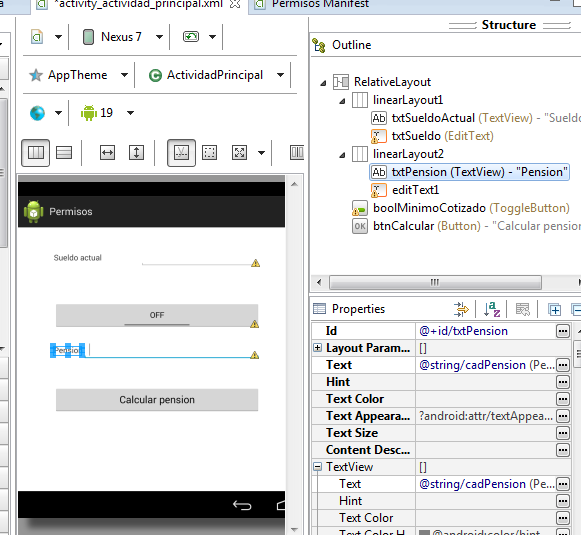
\includegraphics{appPension.png}
\caption{Interfaz de la aplicación}\end{figure}

La aplicación calcula una pensión de una forma muy sencilla: si se ha cotizado durante el mínimo de años exigidos por la ley, se tiene una pensión equivalente al 90\% del sueldo actual. Si no ha sido así se tiene una pensión del 75\% del sueldo actual.

Aunque es una funcionalidad que todavía no se va a implementar, la app podrá enviar un SMS con el resultado (y un anuncio de nuestra empresa) a otro número. Esto implica hacer que la aplicación exija pedir ese permiso en el \code{AndroidManifest.xml}.


\subsection{Código Java}
\label{tema2:codigo-java}
El código Java sería algo así (faltan unas líneas)

\begin{Verbatim}[commandchars=\\\{\}]
\PYG{k+kd}{public} \PYG{k+kt}{void} \PYG{n+nf}{calcularPension}\PYG{o}{(}\PYG{n}{View} \PYG{n}{controlPulsado}\PYG{o}{)}\PYG{o}{\PYGZob{}}
                \PYG{n}{EditText} \PYG{n}{control}\PYG{o}{;}
                \PYG{n}{control}\PYG{o}{=}\PYG{o}{(}\PYG{n}{EditText}\PYG{o}{)}
                                \PYG{k}{this}\PYG{o}{.}\PYG{n+na}{findViewById}\PYG{o}{(}\PYG{n}{R}\PYG{o}{.}\PYG{n+na}{id}\PYG{o}{.}\PYG{n+na}{txtSueldoActual}\PYG{o}{)}\PYG{o}{;}

                \PYG{n}{Editable} \PYG{n}{cadPension}\PYG{o}{=}\PYG{n}{control}\PYG{o}{.}\PYG{n+na}{getEditableText}\PYG{o}{(}\PYG{o}{)}\PYG{o}{;}
                \PYG{k}{if} \PYG{o}{(}\PYG{n}{cadPension}\PYG{o}{.}\PYG{n+na}{toString}\PYG{o}{(}\PYG{o}{)}\PYG{o}{.}\PYG{n+na}{equals}\PYG{o}{(}\PYG{l+s}{\PYGZdq{}\PYGZdq{}}\PYG{o}{)}\PYG{o}{)} \PYG{k}{return} \PYG{o}{;}
                \PYG{n}{Double} \PYG{n}{sueldoActual}\PYG{o}{;}
                \PYG{n}{sueldoActual}\PYG{o}{=}
                                \PYG{n}{Double}\PYG{o}{.}\PYG{n+na}{parseDouble}\PYG{o}{(}\PYG{n}{cadPension}\PYG{o}{.}\PYG{n+na}{toString}\PYG{o}{(}\PYG{o}{)}\PYG{o}{)}\PYG{o}{;}

                \PYG{n}{ToggleButton} \PYG{n}{togMinimo}\PYG{o}{;}
                \PYG{n}{togMinimo}\PYG{o}{=}\PYG{o}{(}\PYG{n}{ToggleButton}\PYG{o}{)}
                                \PYG{k}{this}\PYG{o}{.}\PYG{n+na}{findViewById}\PYG{o}{(}\PYG{n}{R}\PYG{o}{.}\PYG{n+na}{id}\PYG{o}{.}\PYG{n+na}{togMinimo}\PYG{o}{)}\PYG{o}{;}
                \PYG{n}{Double} \PYG{n}{pensionResultado}\PYG{o}{;}
                \PYG{k}{if} \PYG{o}{(}\PYG{n}{togMinimo}\PYG{o}{.}\PYG{n+na}{isChecked}\PYG{o}{(}\PYG{o}{)}\PYG{o}{)}\PYG{o}{\PYGZob{}}
                        \PYG{n}{pensionResultado}\PYG{o}{=}\PYG{n}{sueldoActual}\PYG{o}{*}\PYG{l+m+mf}{0.9}\PYG{o}{;}
                \PYG{o}{\PYGZcb{}}
                \PYG{k}{else} \PYG{o}{\PYGZob{}}
                        \PYG{n}{pensionResultado}\PYG{o}{=}\PYG{n}{sueldoActual}\PYG{o}{*}\PYG{l+m+mf}{0.75}\PYG{o}{;}
                \PYG{o}{\PYGZcb{}}

                \PYG{n}{EditText} \PYG{n}{txtPensionResultado}\PYG{o}{;}
                \PYG{n}{txtPensionResultado}\PYG{o}{=}\PYG{o}{(}\PYG{n}{EditText}\PYG{o}{)}
                                \PYG{k}{this}\PYG{o}{.}\PYG{n+na}{findViewById}\PYG{o}{(}\PYG{n}{R}\PYG{o}{.}\PYG{n+na}{id}\PYG{o}{.}\PYG{n+na}{txtPensionResultado}\PYG{o}{)}\PYG{o}{;}
                \PYG{n}{txtPensionResultado}\PYG{o}{.}\PYG{n+na}{setText}\PYG{o}{(}\PYG{n}{pensionResultado}\PYG{o}{.}\PYG{n+na}{toString}\PYG{o}{(}\PYG{o}{)}\PYG{o}{)}\PYG{o}{;}
        \PYG{o}{\PYGZcb{}}
\end{Verbatim}


\section{Sobre el diseño de interfaces}
\label{tema2:sobre-el-diseno-de-interfaces}
Cuando se diseña un interfaz lo normal es ir insertando los controles en ``layouts'' que a su vez van dentro de otros. El objetivo es poder modificar un bloque de controles sin afectar a los demás.

Todo control Android puede manipularse de dos formas:
\begin{itemize}
\item {} 
Indicando su tamaño en los parámetros \code{width} y \code{height}. Se podría indicar el tamaño en puntos (mala idea porque el control no se redimensiona automáticamente) pero también se pueden indicar otras dos posibilidades:
\begin{itemize}
\item {} 
\code{wrap\_content}: significa más o menos ``adáptate al mínimo posible''.

\item {} 
\code{match\_parent}: ``agrándate y adáptate al tamaño de tu contenedor padre''.

\end{itemize}

\item {} 
Indicando qué proporción ocupa con respecto a sus controles del mismo contenedor. Esto se hace modificando el atributo \code{weight} y poniendo luego el \code{width} o el \code{height} a \code{0dp}.

\end{itemize}


\subsection{Ejercicio}
\label{tema2:id1}
Crear una aplicación que permita al usuario practicar el cálculo mental con operaciones sencillas (sumas y restas) con números pequeños (de 1 a 99). Cuando el usuario introduce un resultado se le dice si acierta o no y se genera una nueva operación al azar.

\begin{Verbatim}[commandchars=\\\{\}]
\PYG{k+kn}{package} \PYG{n}{com}\PYG{o}{.}\PYG{n+na}{ies}\PYG{o}{.}\PYG{n+na}{calculus}\PYG{o}{;}

\PYG{k+kn}{import} \PYG{n+nn}{java.util.Random}\PYG{o}{;}

\PYG{k+kn}{import} \PYG{n+nn}{android.support.v7.app.ActionBarActivity}\PYG{o}{;}
\PYG{k+kn}{import} \PYG{n+nn}{android.os.Bundle}\PYG{o}{;}
\PYG{k+kn}{import} \PYG{n+nn}{android.util.Log}\PYG{o}{;}
\PYG{k+kn}{import} \PYG{n+nn}{android.view.Menu}\PYG{o}{;}
\PYG{k+kn}{import} \PYG{n+nn}{android.view.MenuItem}\PYG{o}{;}
\PYG{k+kn}{import} \PYG{n+nn}{android.view.View}\PYG{o}{;}
\PYG{k+kn}{import} \PYG{n+nn}{android.widget.EditText}\PYG{o}{;}
\PYG{k+kn}{import} \PYG{n+nn}{android.widget.TextView}\PYG{o}{;}


\PYG{k+kd}{public} \PYG{k+kd}{class} \PYG{n+nc}{ActividadPrincipal} \PYG{k+kd}{extends} \PYG{n}{ActionBarActivity} \PYG{o}{\PYGZob{}}
        \PYG{k+kt}{int} \PYG{n}{num1}\PYG{o}{;}
        \PYG{k+kt}{int} \PYG{n}{num2}\PYG{o}{;}
        \PYG{n}{String} \PYG{n}{operacion}\PYG{o}{;}
        \PYG{n+nd}{@Override}
        \PYG{k+kd}{protected} \PYG{k+kt}{void} \PYG{n+nf}{onCreate}\PYG{o}{(}\PYG{n}{Bundle} \PYG{n}{savedInstanceState}\PYG{o}{)} \PYG{o}{\PYGZob{}}
                \PYG{k+kd}{super}\PYG{o}{.}\PYG{n+na}{onCreate}\PYG{o}{(}\PYG{n}{savedInstanceState}\PYG{o}{)}\PYG{o}{;}
                \PYG{n}{setContentView}\PYG{o}{(}\PYG{n}{R}\PYG{o}{.}\PYG{n+na}{layout}\PYG{o}{.}\PYG{n+na}{activity\PYGZus{}actividad\PYGZus{}principal}\PYG{o}{)}\PYG{o}{;}
                \PYG{n}{generarOperacion}\PYG{o}{(}\PYG{o}{)}\PYG{o}{;}
        \PYG{o}{\PYGZcb{}}


        \PYG{n+nd}{@Override}
        \PYG{k+kd}{public} \PYG{k+kt}{boolean} \PYG{n+nf}{onCreateOptionsMenu}\PYG{o}{(}\PYG{n}{Menu} \PYG{n}{menu}\PYG{o}{)} \PYG{o}{\PYGZob{}}
                \PYG{c+c1}{// Inflate the menu; this adds items to the action bar if it is present.}
                \PYG{n}{getMenuInflater}\PYG{o}{(}\PYG{o}{)}\PYG{o}{.}\PYG{n+na}{inflate}\PYG{o}{(}\PYG{n}{R}\PYG{o}{.}\PYG{n+na}{menu}\PYG{o}{.}\PYG{n+na}{actividad\PYGZus{}principal}\PYG{o}{,} \PYG{n}{menu}\PYG{o}{)}\PYG{o}{;}
                \PYG{k}{return} \PYG{k+kc}{true}\PYG{o}{;}
        \PYG{o}{\PYGZcb{}}

        \PYG{n+nd}{@Override}
        \PYG{k+kd}{public} \PYG{k+kt}{boolean} \PYG{n+nf}{onOptionsItemSelected}\PYG{o}{(}\PYG{n}{MenuItem} \PYG{n}{item}\PYG{o}{)} \PYG{o}{\PYGZob{}}
                \PYG{c+c1}{// Handle action bar item clicks here. The action bar will}
                \PYG{c+c1}{// automatically handle clicks on the Home/Up button, so long}
                \PYG{c+c1}{// as you specify a parent activity in AndroidManifest.xml.}
                \PYG{k+kt}{int} \PYG{n}{id} \PYG{o}{=} \PYG{n}{item}\PYG{o}{.}\PYG{n+na}{getItemId}\PYG{o}{(}\PYG{o}{)}\PYG{o}{;}
                \PYG{k}{if} \PYG{o}{(}\PYG{n}{id} \PYG{o}{=}\PYG{o}{=} \PYG{n}{R}\PYG{o}{.}\PYG{n+na}{id}\PYG{o}{.}\PYG{n+na}{action\PYGZus{}settings}\PYG{o}{)} \PYG{o}{\PYGZob{}}
                        \PYG{k}{return} \PYG{k+kc}{true}\PYG{o}{;}
                \PYG{o}{\PYGZcb{}}
                \PYG{k}{return} \PYG{k+kd}{super}\PYG{o}{.}\PYG{n+na}{onOptionsItemSelected}\PYG{o}{(}\PYG{n}{item}\PYG{o}{)}\PYG{o}{;}
        \PYG{o}{\PYGZcb{}}

        \PYG{k+kd}{private} \PYG{k+kt}{void} \PYG{n+nf}{escribirNumeroEnTextView}\PYG{o}{(}
                        \PYG{k+kt}{int} \PYG{n}{num}\PYG{o}{,} \PYG{k+kt}{int} \PYG{n}{id}\PYG{o}{)}\PYG{o}{\PYGZob{}}
                \PYG{n}{TextView} \PYG{n}{tv}\PYG{o}{=}\PYG{o}{(}\PYG{n}{TextView}\PYG{o}{)}
                                \PYG{k}{this}\PYG{o}{.}\PYG{n+na}{findViewById}\PYG{o}{(}\PYG{n}{id}\PYG{o}{)}\PYG{o}{;}
                \PYG{n}{tv}\PYG{o}{.}\PYG{n+na}{setText}\PYG{o}{(}\PYG{l+s}{\PYGZdq{}\PYGZdq{}}\PYG{o}{+}\PYG{n}{num}\PYG{o}{)}\PYG{o}{;}
        \PYG{o}{\PYGZcb{}}
        \PYG{k+kd}{private} \PYG{k+kt}{void} \PYG{n+nf}{generarOperacion}\PYG{o}{(}\PYG{o}{)}\PYG{o}{\PYGZob{}}
                \PYG{n}{Random} \PYG{n}{generador}\PYG{o}{=}\PYG{k}{new} \PYG{n}{Random}\PYG{o}{(}\PYG{o}{)}\PYG{o}{;}
                \PYG{n}{num1}\PYG{o}{=}\PYG{n}{generador}\PYG{o}{.}\PYG{n+na}{nextInt}\PYG{o}{(}\PYG{l+m+mi}{100}\PYG{o}{)}\PYG{o}{;}
                \PYG{n}{num2}\PYG{o}{=}\PYG{n}{generador}\PYG{o}{.}\PYG{n+na}{nextInt}\PYG{o}{(}\PYG{l+m+mi}{100}\PYG{o}{)}\PYG{o}{;}
                \PYG{n}{escribirNumeroEnTextView}\PYG{o}{(}
                                \PYG{n}{num1}\PYG{o}{,} \PYG{n}{R}\PYG{o}{.}\PYG{n+na}{id}\PYG{o}{.}\PYG{n+na}{tvOperando1}\PYG{o}{)}\PYG{o}{;}
                \PYG{n}{escribirNumeroEnTextView}\PYG{o}{(}
                                \PYG{n}{num2}\PYG{o}{,} \PYG{n}{R}\PYG{o}{.}\PYG{n+na}{id}\PYG{o}{.}\PYG{n+na}{tvOperando2}\PYG{o}{)}\PYG{o}{;}
                \PYG{c+c1}{//Para generar la op. matemática}
                \PYG{c+c1}{//escogeremos un valor al azar de un vector}
                \PYG{n}{String}\PYG{o}{[}\PYG{o}{]} \PYG{n}{ops}\PYG{o}{=}\PYG{o}{\PYGZob{}}\PYG{l+s}{\PYGZdq{}+\PYGZdq{}}\PYG{o}{,} \PYG{l+s}{\PYGZdq{}\PYGZhy{}\PYGZdq{}}\PYG{o}{\PYGZcb{}}\PYG{o}{;}

                \PYG{k+kt}{int} \PYG{n}{posAzar}\PYG{o}{=}\PYG{n}{generador}\PYG{o}{.}\PYG{n+na}{nextInt}\PYG{o}{(}\PYG{n}{ops}\PYG{o}{.}\PYG{n+na}{length}\PYG{o}{)}\PYG{o}{;}
                \PYG{n}{operacion}\PYG{o}{=}\PYG{n}{ops}\PYG{o}{[}\PYG{n}{posAzar}\PYG{o}{]}\PYG{o}{;}
                \PYG{n}{TextView} \PYG{n}{tvOperando}\PYG{o}{=}
                                \PYG{o}{(}\PYG{n}{TextView}\PYG{o}{)}\PYG{k}{this}\PYG{o}{.}\PYG{n+na}{findViewById}\PYG{o}{(}\PYG{n}{R}\PYG{o}{.}\PYG{n+na}{id}\PYG{o}{.}\PYG{n+na}{tvOperador}\PYG{o}{)}\PYG{o}{;}
                \PYG{n}{tvOperando}\PYG{o}{.}\PYG{n+na}{setText}\PYG{o}{(}\PYG{n}{operacion}\PYG{o}{)}\PYG{o}{;}
        \PYG{o}{\PYGZcb{}}
        \PYG{k+kd}{public} \PYG{k+kt}{void} \PYG{n+nf}{comprobar}\PYG{o}{(}\PYG{n}{View} \PYG{n}{control}\PYG{o}{)}\PYG{o}{\PYGZob{}}
                \PYG{n}{EditText} \PYG{n}{txtResultado}\PYG{o}{=}\PYG{o}{(}\PYG{n}{EditText}\PYG{o}{)}
                                \PYG{k}{this}\PYG{o}{.}\PYG{n+na}{findViewById}\PYG{o}{(}\PYG{n}{R}\PYG{o}{.}\PYG{n+na}{id}\PYG{o}{.}\PYG{n+na}{txtResultado}\PYG{o}{)}\PYG{o}{;}
                \PYG{n}{String} \PYG{n}{resultado}\PYG{o}{=}\PYG{n}{txtResultado}\PYG{o}{.}\PYG{n+na}{getText}\PYG{o}{(}\PYG{o}{)}\PYG{o}{.}\PYG{n+na}{toString}\PYG{o}{(}\PYG{o}{)}\PYG{o}{;}
                \PYG{n}{TextView} \PYG{n}{tvMensajes}\PYG{o}{=}\PYG{o}{(}\PYG{n}{TextView}\PYG{o}{)}
                                \PYG{k}{this}\PYG{o}{.}\PYG{n+na}{findViewById}\PYG{o}{(}\PYG{n}{R}\PYG{o}{.}\PYG{n+na}{id}\PYG{o}{.}\PYG{n+na}{tvMensajes}\PYG{o}{)}\PYG{o}{;}
                \PYG{k}{if} \PYG{o}{(}\PYG{n}{resultado}\PYG{o}{.}\PYG{n+na}{equals}\PYG{o}{(}\PYG{l+s}{\PYGZdq{}\PYGZdq{}}\PYG{o}{)}\PYG{o}{)}\PYG{o}{\PYGZob{}}
                        \PYG{n}{tvMensajes}\PYG{o}{.}\PYG{n+na}{setText}\PYG{o}{(}\PYG{l+s}{\PYGZdq{}Resultado incorrecto\PYGZdq{}}\PYG{o}{)}\PYG{o}{;}
                        \PYG{n}{generarOperacion}\PYG{o}{(}\PYG{o}{)}\PYG{o}{;}
                        \PYG{k}{return} \PYG{o}{;}
                \PYG{o}{\PYGZcb{}}
                \PYG{k+kt}{int} \PYG{n}{resultCalculado}\PYG{o}{=}\PYG{l+m+mi}{0}\PYG{o}{;}
                \PYG{k}{switch} \PYG{o}{(}\PYG{n}{operacion}\PYG{o}{.}\PYG{n+na}{charAt}\PYG{o}{(}\PYG{l+m+mi}{0}\PYG{o}{)}\PYG{o}{)}\PYG{o}{\PYGZob{}}
                        \PYG{k}{case} \PYG{l+s+sc}{\PYGZsq{}+\PYGZsq{}}\PYG{o}{:}\PYG{o}{\PYGZob{}}
                                \PYG{n}{resultCalculado}\PYG{o}{=}\PYG{n}{num1}\PYG{o}{+}\PYG{n}{num2}\PYG{o}{;}
                                \PYG{k}{break}\PYG{o}{;}
                        \PYG{o}{\PYGZcb{}}
                        \PYG{k}{case} \PYG{l+s+sc}{\PYGZsq{}\PYGZhy{}\PYGZsq{}}\PYG{o}{:}\PYG{o}{\PYGZob{}}
                                \PYG{n}{resultCalculado}\PYG{o}{=}\PYG{n}{num1}\PYG{o}{\PYGZhy{}}\PYG{n}{num2}\PYG{o}{;}
                                \PYG{k}{break}\PYG{o}{;}
                        \PYG{o}{\PYGZcb{}}
                \PYG{o}{\PYGZcb{}}
                \PYG{k+kt}{int} \PYG{n}{resultadoIntroducido}\PYG{o}{=}
                                \PYG{n}{Integer}\PYG{o}{.}\PYG{n+na}{parseInt}\PYG{o}{(}\PYG{n}{resultado}\PYG{o}{)}\PYG{o}{;}
                \PYG{k}{if} \PYG{o}{(}\PYG{n}{resultadoIntroducido}\PYG{o}{=}\PYG{o}{=}\PYG{n}{resultCalculado}\PYG{o}{)}\PYG{o}{\PYGZob{}}
                        \PYG{n}{tvMensajes}\PYG{o}{.}\PYG{n+na}{setText}\PYG{o}{(}\PYG{l+s}{\PYGZdq{}¡Correcto!\PYGZdq{}}\PYG{o}{)}\PYG{o}{;}
                \PYG{o}{\PYGZcb{}} \PYG{k}{else} \PYG{o}{\PYGZob{}}
                        \PYG{n}{tvMensajes}\PYG{o}{.}\PYG{n+na}{setText}\PYG{o}{(}\PYG{l+s}{\PYGZdq{}¡MAL!\PYGZdq{}}\PYG{o}{)}\PYG{o}{;}
                \PYG{o}{\PYGZcb{}}
                \PYG{n}{txtResultado}\PYG{o}{.}\PYG{n+na}{setText}\PYG{o}{(}\PYG{l+s}{\PYGZdq{}\PYGZdq{}}\PYG{o}{)}\PYG{o}{;}
                \PYG{n}{generarOperacion}\PYG{o}{(}\PYG{o}{)}\PYG{o}{;}
        \PYG{o}{\PYGZcb{}}
\PYG{o}{\PYGZcb{}}
\end{Verbatim}


\subsection{Resumen de los contenedores Android}
\label{tema2:resumen-de-los-contenedores-android}
En la imagen siguiente puede apreciarse la variedad de contenedores que ofrece Android:
\begin{figure}[htbp]
\centering
\capstart

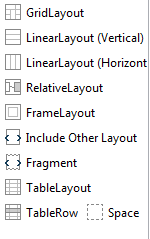
\includegraphics{contenedores.png}
\caption{Contenedores Android}\end{figure}


\section{Actividades}
\label{tema2:actividades}
Una actividad es un programa diseñado no solo para llamar a otros programas sino que también puede ofrecer sus servicios en Android para que otros programas les llamen a ellos.

El objetivo básico es comprender la forma de comunicar actividades en Android.


\subsection{Actividad receptora de información}
\label{tema2:actividad-receptora-de-informacion}
Una actividad típica debería estar preparada para recibir parámetros de una forma similar a esta:

\begin{Verbatim}[commandchars=\\\{\}]
\PYG{k+kd}{public} \PYG{k+kd}{static} \PYG{n}{String} \PYG{n}{parametroNombre}\PYG{o}{=}
                \PYG{l+s}{\PYGZdq{}com.ies.actividades1.nombrePersona\PYGZdq{}}\PYG{o}{;}
\PYG{k+kd}{protected} \PYG{k+kt}{void} \PYG{n+nf}{onCreate}\PYG{o}{(}\PYG{n}{Bundle} \PYG{n}{savedInstanceState}\PYG{o}{)} \PYG{o}{\PYGZob{}}
        \PYG{k+kd}{super}\PYG{o}{.}\PYG{n+na}{onCreate}\PYG{o}{(}\PYG{n}{savedInstanceState}\PYG{o}{)}\PYG{o}{;}
        \PYG{k}{this}\PYG{o}{.}\PYG{n+na}{setContentView}\PYG{o}{(}\PYG{n}{R}\PYG{o}{.}\PYG{n+na}{layout}\PYG{o}{.}\PYG{n+na}{actividad\PYGZus{}mostrar\PYGZus{}nombres}\PYG{o}{)}\PYG{o}{;}

        \PYG{n}{Intent} \PYG{n}{intentPasado}\PYG{o}{=}\PYG{k}{this}\PYG{o}{.}\PYG{n+na}{getIntent}\PYG{o}{(}\PYG{o}{)}\PYG{o}{;}
        \PYG{n}{String} \PYG{n}{nombrePasado}\PYG{o}{=}
                        \PYG{n}{intentPasado}\PYG{o}{.}\PYG{n+na}{getStringExtra}\PYG{o}{(}
                \PYG{n}{ActividadMostrarNombres}\PYG{o}{.}\PYG{n+na}{parametroNombre}
        \PYG{o}{)}\PYG{o}{;}

        \PYG{n}{TextView} \PYG{n}{txtNombreAMostrar}\PYG{o}{;}
        \PYG{n}{txtNombreAMostrar}\PYG{o}{=}
                        \PYG{o}{(}\PYG{n}{TextView}\PYG{o}{)} \PYG{k}{this}\PYG{o}{.}\PYG{n+na}{findViewById}\PYG{o}{(}\PYG{n}{R}\PYG{o}{.}\PYG{n+na}{id}\PYG{o}{.}\PYG{n+na}{txtNombreMostrado}\PYG{o}{)}\PYG{o}{;}
        \PYG{n}{txtNombreAMostrar}\PYG{o}{.}\PYG{n+na}{setText}\PYG{o}{(}\PYG{n}{nombrePasado}\PYG{o}{)}\PYG{o}{;}
\PYG{o}{\PYGZcb{}}
\end{Verbatim}


\subsection{Actividad llamadora}
\label{tema2:actividad-llamadora}
Una actividad que desee invocar a otro necesitará ``pasar parámetros'' de una forma similar a esta:

\begin{Verbatim}[commandchars=\\\{\}]
    \PYG{k+kd}{public} \PYG{k+kt}{void} \PYG{n+nf}{pasarNombre}\PYG{o}{(}\PYG{n}{View} \PYG{n}{control}\PYG{o}{)}\PYG{o}{\PYGZob{}}
    \PYG{n}{EditText} \PYG{n}{txtNombre}\PYG{o}{;}
    \PYG{n}{txtNombre}\PYG{o}{=}\PYG{o}{(}\PYG{n}{EditText}\PYG{o}{)} \PYG{n}{findViewById}\PYG{o}{(}\PYG{n}{R}\PYG{o}{.}\PYG{n+na}{id}\PYG{o}{.}\PYG{n+na}{txtNombre}\PYG{o}{)}\PYG{o}{;}
    \PYG{n}{String} \PYG{n}{nombre}\PYG{o}{=}\PYG{n}{txtNombre}\PYG{o}{.}\PYG{n+na}{getText}\PYG{o}{(}\PYG{o}{)}\PYG{o}{.}\PYG{n+na}{toString}\PYG{o}{(}\PYG{o}{)}\PYG{o}{;}
    \PYG{n}{Intent} \PYG{n}{iMostrarNombre}\PYG{o}{;}
    \PYG{c+c1}{//Indicamos quien es el llamador e}
    \PYG{c+c1}{//indicamos}
    \PYG{n}{iMostrarNombre}\PYG{o}{=}\PYG{k}{new} \PYG{n}{Intent}\PYG{o}{(}
                    \PYG{k}{this}\PYG{o}{,} \PYG{n}{ActividadMostrarNombres}\PYG{o}{.}\PYG{n+na}{class}\PYG{o}{)}\PYG{o}{;}
    \PYG{n}{iMostrarNombre}\PYG{o}{.}\PYG{n+na}{putExtra}
            \PYG{o}{(}\PYG{n}{ActividadMostrarNombres}\PYG{o}{.}\PYG{n+na}{parametroNombre}
                            \PYG{o}{,} \PYG{n}{nombre}\PYG{o}{)}\PYG{o}{;}
    \PYG{c+c1}{//Se lanza el intent}
    \PYG{k}{this}\PYG{o}{.}\PYG{n+na}{startActivity}\PYG{o}{(}\PYG{n}{iMostrarNombre}\PYG{o}{)}\PYG{o}{;}

\PYG{o}{\PYGZcb{}}
\end{Verbatim}


\section{Construcción de actividades}
\label{tema2:construccion-de-actividades}
Para crear una actividad desde cero necesitamos hacer dos cosas
\begin{enumerate}
\item {} 
Crear el interfaz XML (Eclipse puede que no añada un \code{id} a dicho interfaz, si no lo ha hecho añadirlo a mano)

\item {} 
Crear una clase Java que herede de \code{Activity}. Dicha clase Java necesita que añadamos algo: el \code{onCreate} contendrá ahora el código que procesa el \code{Intent} que nos pasen y también  usaremos \code{setContentView} para cargar un fichero de interfaz o \emph{layout}.

\end{enumerate}

Dentro de la actividad suele ser buena política definir los nombres de los parámetros utilizando como prefijo el nombre del paquete:

\begin{Verbatim}[commandchars=\\\{\}]
\PYG{k+kd}{public} \PYG{k+kd}{class}
        \PYG{n+nc}{ActividadCalculadora} \PYG{k+kd}{extends} \PYG{n}{Activity} \PYG{o}{\PYGZob{}}

        \PYG{k+kd}{public} \PYG{k+kd}{static} \PYG{n}{String} \PYG{n}{nombreNum1}\PYG{o}{=}
                        \PYG{l+s}{\PYGZdq{}com.ies.actividades2.num1\PYGZdq{}}\PYG{o}{;}
        \PYG{k+kd}{public} \PYG{k+kd}{static} \PYG{n}{String} \PYG{n}{nombreNum2}\PYG{o}{=}
                        \PYG{l+s}{\PYGZdq{}com.ies.actividades2.num2\PYGZdq{}}\PYG{o}{;}
        \PYG{k+kd}{public} \PYG{k+kd}{static} \PYG{n}{String} \PYG{n}{nombreOp}\PYG{o}{=}
                        \PYG{l+s}{\PYGZdq{}com.ies.actividades2.op\PYGZdq{}}\PYG{o}{;}
        \PYG{n+nd}{@Override}
        \PYG{k+kd}{protected} \PYG{k+kt}{void} \PYG{n+nf}{onCreate}\PYG{o}{(}\PYG{n}{Bundle} \PYG{n}{savedInstanceState}\PYG{o}{)} \PYG{o}{\PYGZob{}}
                \PYG{c+c1}{// TODO Auto\PYGZhy{}generated method stub}
                \PYG{k+kd}{super}\PYG{o}{.}\PYG{n+na}{onCreate}\PYG{o}{(}\PYG{n}{savedInstanceState}\PYG{o}{)}\PYG{o}{;}

        \PYG{o}{\PYGZcb{}}
\PYG{o}{\PYGZcb{}}
\end{Verbatim}


\section{Ejemplo: llamadas entre actividades}
\label{tema2:ejemplo-llamadas-entre-actividades}
Supongamos que deseamos tener una actividad que acepta recibir dos números y un operando. Tras la recepción se efectuará la operación matemática y se mostrará el resultado en un interfaz distinto de la actividad llamadora.
\begin{figure}[htbp]
\centering
\capstart

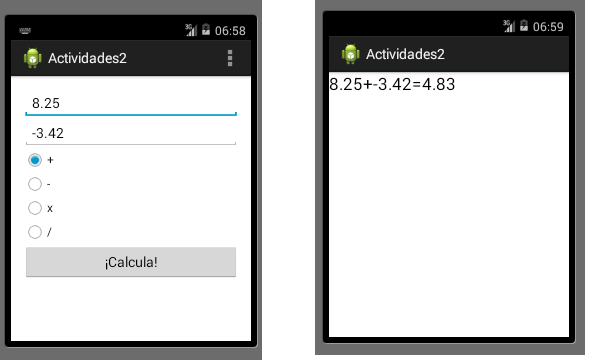
\includegraphics{actividadcalculadora.png}
\caption{Aplicación con dos actividades}\end{figure}


\subsection{Actividad calculadora}
\label{tema2:actividad-calculadora}
Esta actividad carga el interfaz XML y despues procesa el \code{Intent} para determinar qué operación debe ejecutar.

También define el nombre de los parámetros en \textbf{constantes} que tanto el llamador como ella pueden usar (y así evitar el cortar y pegar).

\begin{Verbatim}[commandchars=\\\{\}]
\PYG{k+kd}{public} \PYG{k+kd}{class} \PYG{n+nc}{ActividadCalculadora} \PYG{k+kd}{extends} \PYG{n}{Activity} \PYG{o}{\PYGZob{}}

        \PYG{k+kd}{public} \PYG{k+kd}{static} \PYG{n}{String} \PYG{n}{nombreNum1}\PYG{o}{=}
                        \PYG{l+s}{\PYGZdq{}com.ies.actividades2.num1\PYGZdq{}}\PYG{o}{;}
        \PYG{k+kd}{public} \PYG{k+kd}{static} \PYG{n}{String} \PYG{n}{nombreNum2}\PYG{o}{=}
                        \PYG{l+s}{\PYGZdq{}com.ies.actividades2.num2\PYGZdq{}}\PYG{o}{;}
        \PYG{k+kd}{public} \PYG{k+kd}{static} \PYG{n}{String} \PYG{n}{nombreOp}\PYG{o}{=}
                        \PYG{l+s}{\PYGZdq{}com.ies.actividades2.op\PYGZdq{}}\PYG{o}{;}
        \PYG{n+nd}{@Override}
        \PYG{k+kd}{protected} \PYG{k+kt}{void} \PYG{n+nf}{onCreate}\PYG{o}{(}\PYG{n}{Bundle} \PYG{n}{savedInstanceState}\PYG{o}{)} \PYG{o}{\PYGZob{}}
                \PYG{c+c1}{// TODO Auto\PYGZhy{}generated method stub}
                \PYG{k+kd}{super}\PYG{o}{.}\PYG{n+na}{onCreate}\PYG{o}{(}\PYG{n}{savedInstanceState}\PYG{o}{)}\PYG{o}{;}
                \PYG{k}{this}\PYG{o}{.}\PYG{n+na}{setContentView}\PYG{o}{(}\PYG{n}{R}\PYG{o}{.}\PYG{n+na}{layout}\PYG{o}{.}\PYG{n+na}{actividad\PYGZus{}secundaria}\PYG{o}{)}\PYG{o}{;}
                \PYG{n}{Intent} \PYG{n}{intento}\PYG{o}{=}\PYG{k}{this}\PYG{o}{.}\PYG{n+na}{getIntent}\PYG{o}{(}\PYG{o}{)}\PYG{o}{;}
                \PYG{k+kt}{float} \PYG{n}{num1}\PYG{o}{=}
                                \PYG{n}{intento}\PYG{o}{.}\PYG{n+na}{getFloatExtra}\PYG{o}{(}
                                                \PYG{n}{ActividadCalculadora}\PYG{o}{.}\PYG{n+na}{nombreNum1}
                                                \PYG{o}{,}
                                                \PYG{l+m+mf}{0.0f}\PYG{o}{)}\PYG{o}{;}
                \PYG{k+kt}{float} \PYG{n}{num2}\PYG{o}{=}\PYG{n}{intento}\PYG{o}{.}\PYG{n+na}{getFloatExtra}\PYG{o}{(}
                                \PYG{n}{ActividadCalculadora}\PYG{o}{.}\PYG{n+na}{nombreNum2}
                                \PYG{o}{,}
                                \PYG{l+m+mf}{0.0f}\PYG{o}{)}\PYG{o}{;}
                \PYG{n}{String} \PYG{n}{op}\PYG{o}{=}
                                \PYG{n}{intento}\PYG{o}{.}\PYG{n+na}{getStringExtra}\PYG{o}{(}
                                                \PYG{n}{ActividadCalculadora}\PYG{o}{.}\PYG{n+na}{nombreOp}\PYG{o}{)}\PYG{o}{;}

                \PYG{k+kt}{float} \PYG{n}{resultado}\PYG{o}{=}\PYG{k}{this}\PYG{o}{.}\PYG{n+na}{calcular}\PYG{o}{(}\PYG{n}{num1}\PYG{o}{,} \PYG{n}{op}\PYG{o}{,} \PYG{n}{num2}\PYG{o}{)}\PYG{o}{;}

                \PYG{n}{String} \PYG{n}{cadResultado}\PYG{o}{=}
                                \PYG{n}{num1}\PYG{o}{+}\PYG{n}{op}\PYG{o}{+}\PYG{n}{num2}\PYG{o}{+}\PYG{l+s}{\PYGZdq{}=\PYGZdq{}}\PYG{o}{+}\PYG{n}{resultado}\PYG{o}{;}
                \PYG{n}{TextView} \PYG{n}{tvResultado}\PYG{o}{;}
                \PYG{n}{tvResultado}\PYG{o}{=}\PYG{o}{(}\PYG{n}{TextView}\PYG{o}{)} \PYG{n}{findViewById}\PYG{o}{(}\PYG{n}{R}\PYG{o}{.}\PYG{n+na}{id}\PYG{o}{.}\PYG{n+na}{tvResultado}\PYG{o}{)}\PYG{o}{;}
                \PYG{n}{tvResultado}\PYG{o}{.}\PYG{n+na}{setText}\PYG{o}{(}\PYG{n}{cadResultado}\PYG{o}{)}\PYG{o}{;}
        \PYG{o}{\PYGZcb{}}
        \PYG{k+kd}{public} \PYG{k+kt}{float} \PYG{n+nf}{calcular}\PYG{o}{(}\PYG{k+kt}{float} \PYG{n}{n1}\PYG{o}{,} \PYG{n}{String} \PYG{n}{op}\PYG{o}{,} \PYG{k+kt}{float} \PYG{n}{n2}\PYG{o}{)}\PYG{o}{\PYGZob{}}
                \PYG{k+kt}{float} \PYG{n}{resultado}\PYG{o}{=}\PYG{l+m+mf}{0.0f}\PYG{o}{;}

                \PYG{k}{if} \PYG{o}{(}\PYG{n}{op}\PYG{o}{.}\PYG{n+na}{equals}\PYG{o}{(}\PYG{l+s}{\PYGZdq{}+\PYGZdq{}}\PYG{o}{)}\PYG{o}{)}\PYG{o}{\PYGZob{}}
                        \PYG{k}{return} \PYG{n}{n1}\PYG{o}{+}\PYG{n}{n2}\PYG{o}{;}
                \PYG{o}{\PYGZcb{}}
                \PYG{k}{if} \PYG{o}{(}\PYG{n}{op}\PYG{o}{.}\PYG{n+na}{equals}\PYG{o}{(}\PYG{l+s}{\PYGZdq{}\PYGZhy{}\PYGZdq{}}\PYG{o}{)}\PYG{o}{)}\PYG{o}{\PYGZob{}}
                        \PYG{k}{return} \PYG{n}{n1}\PYG{o}{\PYGZhy{}}\PYG{n}{n2}\PYG{o}{;}
                \PYG{o}{\PYGZcb{}}
                \PYG{k}{return} \PYG{n}{resultado}\PYG{o}{;}
        \PYG{o}{\PYGZcb{}}
\PYG{o}{\PYGZcb{}}
\end{Verbatim}


\subsection{Actividad llamadora}
\label{tema2:id2}
\begin{Verbatim}[commandchars=\\\{\}]
\PYG{k+kd}{public} \PYG{k+kd}{class} \PYG{n+nc}{ActividadPrincipal} \PYG{k+kd}{extends} \PYG{n}{ActionBarActivity} \PYG{o}{\PYGZob{}}

        \PYG{n+nd}{@Override}
        \PYG{k+kd}{protected} \PYG{k+kt}{void} \PYG{n+nf}{onCreate}\PYG{o}{(}\PYG{n}{Bundle} \PYG{n}{savedInstanceState}\PYG{o}{)} \PYG{o}{\PYGZob{}}
                \PYG{k+kd}{super}\PYG{o}{.}\PYG{n+na}{onCreate}\PYG{o}{(}\PYG{n}{savedInstanceState}\PYG{o}{)}\PYG{o}{;}
                \PYG{n}{setContentView}\PYG{o}{(}\PYG{n}{R}\PYG{o}{.}\PYG{n+na}{layout}\PYG{o}{.}\PYG{n+na}{activity\PYGZus{}actividad\PYGZus{}principal}\PYG{o}{)}\PYG{o}{;}
        \PYG{o}{\PYGZcb{}}


        \PYG{n+nd}{@Override}
        \PYG{k+kd}{public} \PYG{k+kt}{boolean} \PYG{n+nf}{onCreateOptionsMenu}\PYG{o}{(}\PYG{n}{Menu} \PYG{n}{menu}\PYG{o}{)} \PYG{o}{\PYGZob{}}
                \PYG{c+c1}{// Inflate the menu; this adds items to the action bar if it is present.}
                \PYG{n}{getMenuInflater}\PYG{o}{(}\PYG{o}{)}\PYG{o}{.}\PYG{n+na}{inflate}\PYG{o}{(}\PYG{n}{R}\PYG{o}{.}\PYG{n+na}{menu}\PYG{o}{.}\PYG{n+na}{actividad\PYGZus{}principal}\PYG{o}{,} \PYG{n}{menu}\PYG{o}{)}\PYG{o}{;}
                \PYG{k}{return} \PYG{k+kc}{true}\PYG{o}{;}
        \PYG{o}{\PYGZcb{}}

        \PYG{n+nd}{@Override}
        \PYG{k+kd}{public} \PYG{k+kt}{boolean} \PYG{n+nf}{onOptionsItemSelected}\PYG{o}{(}\PYG{n}{MenuItem} \PYG{n}{item}\PYG{o}{)} \PYG{o}{\PYGZob{}}
                \PYG{c+c1}{// Handle action bar item clicks here. The action bar will}
                \PYG{c+c1}{// automatically handle clicks on the Home/Up button, so long}
                \PYG{c+c1}{// as you specify a parent activity in AndroidManifest.xml.}
                \PYG{k+kt}{int} \PYG{n}{id} \PYG{o}{=} \PYG{n}{item}\PYG{o}{.}\PYG{n+na}{getItemId}\PYG{o}{(}\PYG{o}{)}\PYG{o}{;}
                \PYG{k}{if} \PYG{o}{(}\PYG{n}{id} \PYG{o}{=}\PYG{o}{=} \PYG{n}{R}\PYG{o}{.}\PYG{n+na}{id}\PYG{o}{.}\PYG{n+na}{action\PYGZus{}settings}\PYG{o}{)} \PYG{o}{\PYGZob{}}
                        \PYG{k}{return} \PYG{k+kc}{true}\PYG{o}{;}
                \PYG{o}{\PYGZcb{}}
                \PYG{k}{return} \PYG{k+kd}{super}\PYG{o}{.}\PYG{n+na}{onOptionsItemSelected}\PYG{o}{(}\PYG{n}{item}\PYG{o}{)}\PYG{o}{;}
        \PYG{o}{\PYGZcb{}}



        \PYG{c+cm}{/* Dado un id de recurso este método nos}
\PYG{c+cm}{         * devuelve el texto que hay dentro}
\PYG{c+cm}{         */}
        \PYG{k+kd}{public} \PYG{k+kt}{float} \PYG{n+nf}{getNumero}\PYG{o}{(}\PYG{k+kt}{int} \PYG{n}{id}\PYG{o}{)}\PYG{o}{\PYGZob{}}
                \PYG{n}{EditText} \PYG{n}{control}\PYG{o}{;}
                \PYG{n}{control}\PYG{o}{=}\PYG{o}{(}\PYG{n}{EditText}\PYG{o}{)} \PYG{n}{findViewById}\PYG{o}{(}\PYG{n}{id}\PYG{o}{)}\PYG{o}{;}
                \PYG{n}{String} \PYG{n}{cadena}\PYG{o}{=}\PYG{n}{control}\PYG{o}{.}\PYG{n+na}{getText}\PYG{o}{(}\PYG{o}{)}\PYG{o}{.}\PYG{n+na}{toString}\PYG{o}{(}\PYG{o}{)}\PYG{o}{;}
                \PYG{k+kt}{float} \PYG{n}{f}\PYG{o}{=}\PYG{n}{Float}\PYG{o}{.}\PYG{n+na}{parseFloat}\PYG{o}{(}\PYG{n}{cadena}\PYG{o}{)}\PYG{o}{;}
                \PYG{k}{return} \PYG{n}{f}\PYG{o}{;}
        \PYG{o}{\PYGZcb{}}
        \PYG{k+kd}{public} \PYG{k+kt}{void} \PYG{n+nf}{lanzarActCalculadora}\PYG{o}{(}
                        \PYG{k+kt}{float} \PYG{n}{f1}\PYG{o}{,} \PYG{k+kt}{float} \PYG{n}{f2}\PYG{o}{,} \PYG{n}{String} \PYG{n}{op}
                        \PYG{o}{)}\PYG{o}{\PYGZob{}}
                \PYG{n}{Intent} \PYG{n}{intento}\PYG{o}{=}\PYG{k}{new} \PYG{n}{Intent}\PYG{o}{(}\PYG{k}{this}\PYG{o}{,} \PYG{n}{ActividadCalculadora}\PYG{o}{.}\PYG{n+na}{class}\PYG{o}{)}\PYG{o}{;}
                \PYG{n}{intento}\PYG{o}{.}\PYG{n+na}{putExtra}\PYG{o}{(}
                                \PYG{n}{ActividadCalculadora}\PYG{o}{.}\PYG{n+na}{nombreNum1}\PYG{o}{,}
                                \PYG{n}{f1}\PYG{o}{)}\PYG{o}{;}
                \PYG{n}{intento}\PYG{o}{.}\PYG{n+na}{putExtra}\PYG{o}{(}
                                \PYG{n}{ActividadCalculadora}\PYG{o}{.}\PYG{n+na}{nombreNum2}\PYG{o}{,}
                                \PYG{n}{f2}\PYG{o}{)}\PYG{o}{;}
                \PYG{n}{intento}\PYG{o}{.}\PYG{n+na}{putExtra}\PYG{o}{(}
                                \PYG{n}{ActividadCalculadora}\PYG{o}{.}\PYG{n+na}{nombreOp}\PYG{o}{,}
                                \PYG{n}{op}\PYG{o}{)}\PYG{o}{;}
                \PYG{k}{this}\PYG{o}{.}\PYG{n+na}{startActivity}\PYG{o}{(}\PYG{n}{intento}\PYG{o}{)}\PYG{o}{;}
        \PYG{o}{\PYGZcb{}}
        \PYG{k+kd}{public} \PYG{k+kt}{void} \PYG{n+nf}{calcular}\PYG{o}{(}\PYG{n}{View} \PYG{n}{control}\PYG{o}{)}\PYG{o}{\PYGZob{}}
                \PYG{n}{RadioButton} \PYG{n}{rbSuma}\PYG{o}{;}
                \PYG{n}{rbSuma}\PYG{o}{=}\PYG{o}{(}\PYG{n}{RadioButton}\PYG{o}{)} \PYG{n}{findViewById}\PYG{o}{(}\PYG{n}{R}\PYG{o}{.}\PYG{n+na}{id}\PYG{o}{.}\PYG{n+na}{radSuma}\PYG{o}{)}\PYG{o}{;}
                \PYG{k}{if} \PYG{o}{(}\PYG{n}{rbSuma}\PYG{o}{.}\PYG{n+na}{isChecked}\PYG{o}{(}\PYG{o}{)}\PYG{o}{)}\PYG{o}{\PYGZob{}}
                        \PYG{k+kt}{float} \PYG{n}{f1}\PYG{o}{=}\PYG{k}{this}\PYG{o}{.}\PYG{n+na}{getNumero}\PYG{o}{(}\PYG{n}{R}\PYG{o}{.}\PYG{n+na}{id}\PYG{o}{.}\PYG{n+na}{txtNum1}\PYG{o}{)}\PYG{o}{;}
                        \PYG{k+kt}{float} \PYG{n}{f2}\PYG{o}{=}\PYG{k}{this}\PYG{o}{.}\PYG{n+na}{getNumero}\PYG{o}{(}\PYG{n}{R}\PYG{o}{.}\PYG{n+na}{id}\PYG{o}{.}\PYG{n+na}{txtNum2}\PYG{o}{)}\PYG{o}{;}
                        \PYG{n}{lanzarActCalculadora}\PYG{o}{(}\PYG{n}{f1}\PYG{o}{,}\PYG{n}{f2}\PYG{o}{,}\PYG{l+s}{\PYGZdq{}+\PYGZdq{}}\PYG{o}{)}\PYG{o}{;}
                \PYG{o}{\PYGZcb{}}
        \PYG{o}{\PYGZcb{}}
\PYG{o}{\PYGZcb{}}
\end{Verbatim}


\subsection{Modificación del \texttt{AndroidManifest.xml}}
\label{tema2:modificacion-del-androidmanifest-xml}
Se debe añadir esta actividad en el \code{AndroidManifest.xml}

\begin{Verbatim}[commandchars=\\\{\}]
        \PYG{n+nt}{\PYGZlt{}activity}
                \PYG{n+na}{android:name=}\PYG{l+s}{\PYGZdq{}.ActividadCalculadora\PYGZdq{}}\PYG{n+nt}{\PYGZgt{}}
\PYG{n+nt}{\PYGZlt{}/activity\PYGZgt{}}
\end{Verbatim}


\section{Ejercicio}
\label{tema2:id3}
Crear una aplicación con dos actividades donde una de ellas permita introducir un texto y un número y la otra reciba ambos valores. La segunda truncará los \emph{n} primeros caracteres de la cadena y los mostrará en pantalla.
\begin{figure}[htbp]
\centering
\capstart

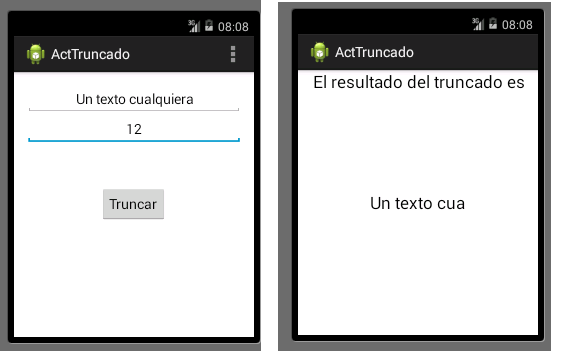
\includegraphics{acttruncado.png}
\caption{Ejemplo de funcionamiento del truncado}\end{figure}


\subsection{Actividad inicial}
\label{tema2:actividad-inicial}
\begin{Verbatim}[commandchars=\\\{\}]
\PYG{k+kd}{public} \PYG{k+kd}{class} \PYG{n+nc}{ActPeticionTexto} \PYG{k+kd}{extends} \PYG{n}{ActionBarActivity} \PYG{o}{\PYGZob{}}

        \PYG{n+nd}{@Override}
        \PYG{k+kd}{protected} \PYG{k+kt}{void} \PYG{n+nf}{onCreate}\PYG{o}{(}\PYG{n}{Bundle} \PYG{n}{savedInstanceState}\PYG{o}{)} \PYG{o}{\PYGZob{}}
                \PYG{k+kd}{super}\PYG{o}{.}\PYG{n+na}{onCreate}\PYG{o}{(}\PYG{n}{savedInstanceState}\PYG{o}{)}\PYG{o}{;}
                \PYG{n}{setContentView}\PYG{o}{(}\PYG{n}{R}\PYG{o}{.}\PYG{n+na}{layout}\PYG{o}{.}\PYG{n+na}{activity\PYGZus{}act\PYGZus{}peticion\PYGZus{}texto}\PYG{o}{)}\PYG{o}{;}
        \PYG{o}{\PYGZcb{}}


        \PYG{n+nd}{@Override}
        \PYG{k+kd}{public} \PYG{k+kt}{boolean} \PYG{n+nf}{onCreateOptionsMenu}\PYG{o}{(}\PYG{n}{Menu} \PYG{n}{menu}\PYG{o}{)} \PYG{o}{\PYGZob{}}
                \PYG{c+c1}{// Inflate the menu; this adds items to the action bar if it is present.}
                \PYG{n}{getMenuInflater}\PYG{o}{(}\PYG{o}{)}\PYG{o}{.}\PYG{n+na}{inflate}\PYG{o}{(}\PYG{n}{R}\PYG{o}{.}\PYG{n+na}{menu}\PYG{o}{.}\PYG{n+na}{act\PYGZus{}peticion\PYGZus{}texto}\PYG{o}{,} \PYG{n}{menu}\PYG{o}{)}\PYG{o}{;}
                \PYG{k}{return} \PYG{k+kc}{true}\PYG{o}{;}
        \PYG{o}{\PYGZcb{}}

        \PYG{n+nd}{@Override}
        \PYG{k+kd}{public} \PYG{k+kt}{boolean} \PYG{n+nf}{onOptionsItemSelected}\PYG{o}{(}\PYG{n}{MenuItem} \PYG{n}{item}\PYG{o}{)} \PYG{o}{\PYGZob{}}
                \PYG{c+c1}{// Handle action bar item clicks here. The action bar will}
                \PYG{c+c1}{// automatically handle clicks on the Home/Up button, so long}
                \PYG{c+c1}{// as you specify a parent activity in AndroidManifest.xml.}
                \PYG{k+kt}{int} \PYG{n}{id} \PYG{o}{=} \PYG{n}{item}\PYG{o}{.}\PYG{n+na}{getItemId}\PYG{o}{(}\PYG{o}{)}\PYG{o}{;}
                \PYG{k}{if} \PYG{o}{(}\PYG{n}{id} \PYG{o}{=}\PYG{o}{=} \PYG{n}{R}\PYG{o}{.}\PYG{n+na}{id}\PYG{o}{.}\PYG{n+na}{action\PYGZus{}settings}\PYG{o}{)} \PYG{o}{\PYGZob{}}
                        \PYG{k}{return} \PYG{k+kc}{true}\PYG{o}{;}
                \PYG{o}{\PYGZcb{}}
                \PYG{k}{return} \PYG{k+kd}{super}\PYG{o}{.}\PYG{n+na}{onOptionsItemSelected}\PYG{o}{(}\PYG{n}{item}\PYG{o}{)}\PYG{o}{;}
        \PYG{o}{\PYGZcb{}}
        \PYG{k+kd}{private} \PYG{n}{String} \PYG{n+nf}{getCadena}\PYG{o}{(}\PYG{k+kt}{int} \PYG{n}{id}\PYG{o}{)}\PYG{o}{\PYGZob{}}
                \PYG{n}{EditText} \PYG{n}{controlTexto}\PYG{o}{=}
                                \PYG{o}{(}\PYG{n}{EditText}\PYG{o}{)} \PYG{k}{this}\PYG{o}{.}\PYG{n+na}{findViewById}\PYG{o}{(}\PYG{n}{id}\PYG{o}{)}\PYG{o}{;}
                \PYG{k}{return} \PYG{n}{controlTexto}\PYG{o}{.}\PYG{n+na}{getText}\PYG{o}{(}\PYG{o}{)}\PYG{o}{.}\PYG{n+na}{toString}\PYG{o}{(}\PYG{o}{)}\PYG{o}{;}
        \PYG{o}{\PYGZcb{}}

        \PYG{k+kd}{public} \PYG{k+kt}{void} \PYG{n+nf}{truncar}\PYG{o}{(}\PYG{n}{View} \PYG{n}{control}\PYG{o}{)}\PYG{o}{\PYGZob{}}
                \PYG{n}{Intent} \PYG{n}{intento}\PYG{o}{=}\PYG{k}{new} \PYG{n}{Intent}\PYG{o}{(}\PYG{k}{this}\PYG{o}{,}\PYG{n}{ActividadTruncadora}\PYG{o}{.}\PYG{n+na}{class}\PYG{o}{)}\PYG{o}{;}
                \PYG{n}{String} \PYG{n}{textoEscrito}\PYG{o}{=}
                                \PYG{n}{getCadena}\PYG{o}{(}\PYG{n}{R}\PYG{o}{.}\PYG{n+na}{id}\PYG{o}{.}\PYG{n+na}{txtTexto}\PYG{o}{)}\PYG{o}{;}
                \PYG{n}{String} \PYG{n}{textoNumCaracteres}\PYG{o}{=}
                                \PYG{n}{getCadena}\PYG{o}{(}\PYG{n}{R}\PYG{o}{.}\PYG{n+na}{id}\PYG{o}{.}\PYG{n+na}{txtNumero}\PYG{o}{)}\PYG{o}{;}
                \PYG{k+kt}{int} \PYG{n}{numCaracteres}\PYG{o}{=}\PYG{n}{Integer}\PYG{o}{.}\PYG{n+na}{parseInt}\PYG{o}{(}
                                \PYG{n}{textoNumCaracteres}\PYG{o}{)}\PYG{o}{;}
                \PYG{n}{intento}\PYG{o}{.}\PYG{n+na}{putExtra}\PYG{o}{(}
                                \PYG{n}{ActividadTruncadora}\PYG{o}{.}\PYG{n+na}{nombreCadena}\PYG{o}{,}
                                \PYG{n}{textoEscrito}\PYG{o}{)}\PYG{o}{;}
                \PYG{n}{intento}\PYG{o}{.}\PYG{n+na}{putExtra}\PYG{o}{(}
                                \PYG{n}{ActividadTruncadora}\PYG{o}{.}\PYG{n+na}{nombreNumCaracteres}\PYG{o}{,}
                                \PYG{n}{numCaracteres}\PYG{o}{)}\PYG{o}{;}
                \PYG{k}{this}\PYG{o}{.}\PYG{n+na}{startActivity}\PYG{o}{(}\PYG{n}{intento}\PYG{o}{)}\PYG{o}{;}
        \PYG{o}{\PYGZcb{}}
\PYG{o}{\PYGZcb{}}
\end{Verbatim}


\subsection{Actividad truncadora}
\label{tema2:actividad-truncadora}
\begin{Verbatim}[commandchars=\\\{\}]
\PYG{k+kd}{public} \PYG{k+kd}{class} \PYG{n+nc}{ActividadTruncadora} \PYG{k+kd}{extends} \PYG{n}{Activity} \PYG{o}{\PYGZob{}}
        \PYG{k+kd}{public} \PYG{k+kd}{static} \PYG{n}{String} \PYG{n}{nombreCadena}\PYG{o}{=}
                        \PYG{l+s}{\PYGZdq{}com.ies.truncado.nombreCadena\PYGZdq{}}\PYG{o}{;}
        \PYG{k+kd}{public} \PYG{k+kd}{static} \PYG{n}{String} \PYG{n}{nombreNumCaracteres}\PYG{o}{=}
                        \PYG{l+s}{\PYGZdq{}com.ies.truncado.nombreNumCaracteres\PYGZdq{}}\PYG{o}{;}
        \PYG{n+nd}{@Override}
        \PYG{k+kd}{protected} \PYG{k+kt}{void} \PYG{n+nf}{onCreate}\PYG{o}{(}\PYG{n}{Bundle} \PYG{n}{savedInstanceState}\PYG{o}{)} \PYG{o}{\PYGZob{}}
                \PYG{c+c1}{// TODO Auto\PYGZhy{}generated method stub}
                \PYG{k+kd}{super}\PYG{o}{.}\PYG{n+na}{onCreate}\PYG{o}{(}\PYG{n}{savedInstanceState}\PYG{o}{)}\PYG{o}{;}
                \PYG{k}{this}\PYG{o}{.}\PYG{n+na}{setContentView}\PYG{o}{(}\PYG{n}{R}\PYG{o}{.}\PYG{n+na}{layout}\PYG{o}{.}\PYG{n+na}{act\PYGZus{}truncado}\PYG{o}{)}\PYG{o}{;}
                \PYG{n}{Intent} \PYG{n}{intRecibido}\PYG{o}{=}\PYG{k}{this}\PYG{o}{.}\PYG{n+na}{getIntent}\PYG{o}{(}\PYG{o}{)}\PYG{o}{;}
                \PYG{n}{String} \PYG{n}{cad}\PYG{o}{=}\PYG{n}{intRecibido}\PYG{o}{.}\PYG{n+na}{getStringExtra}\PYG{o}{(}
                                \PYG{n}{ActividadTruncadora}\PYG{o}{.}\PYG{n+na}{nombreCadena}
                                \PYG{o}{)}\PYG{o}{;}
                \PYG{k+kt}{int} \PYG{n}{numCaracteres}\PYG{o}{=}      \PYG{n}{intRecibido}\PYG{o}{.}\PYG{n+na}{getIntExtra}\PYG{o}{(}
                        \PYG{n}{ActividadTruncadora}\PYG{o}{.}\PYG{n+na}{nombreNumCaracteres}\PYG{o}{,}
                        \PYG{l+m+mi}{0}\PYG{o}{)}\PYG{o}{;}

                \PYG{n}{String} \PYG{n}{cadTruncada}\PYG{o}{=}\PYG{k}{this}\PYG{o}{.}\PYG{n+na}{truncar}\PYG{o}{(}\PYG{n}{cad}\PYG{o}{,} \PYG{n}{numCaracteres}\PYG{o}{)}\PYG{o}{;}
                \PYG{n}{Log}\PYG{o}{.}\PYG{n+na}{d}\PYG{o}{(}\PYG{l+s}{\PYGZdq{}Truncado\PYGZdq{}}\PYG{o}{,} \PYG{l+s}{\PYGZdq{}Resultado:\PYGZdq{}}\PYG{o}{+}\PYG{n}{cadTruncada}\PYG{o}{)}\PYG{o}{;}
                \PYG{n}{TextView} \PYG{n}{tvTextoTruncado}\PYG{o}{=}
                                \PYG{o}{(}\PYG{n}{TextView}\PYG{o}{)} \PYG{k}{this}\PYG{o}{.}\PYG{n+na}{findViewById}\PYG{o}{(}\PYG{n}{R}\PYG{o}{.}\PYG{n+na}{id}\PYG{o}{.}\PYG{n+na}{tvResultado}\PYG{o}{)}\PYG{o}{;}
                \PYG{n}{tvTextoTruncado}\PYG{o}{.}\PYG{n+na}{setText}\PYG{o}{(}\PYG{n}{cadTruncada}\PYG{o}{)}\PYG{o}{;}
        \PYG{o}{\PYGZcb{}}

        \PYG{c+cm}{/* Recorta los num primeros caracteres*/}
        \PYG{k+kd}{private} \PYG{n}{String} \PYG{n+nf}{truncar} \PYG{o}{(}\PYG{n}{String} \PYG{n}{cad}\PYG{o}{,} \PYG{k+kt}{int} \PYG{n}{num}\PYG{o}{)}\PYG{o}{\PYGZob{}}
                \PYG{c+cm}{/* Si el usuario intenta poner}
\PYG{c+cm}{                 * un valor más grande que la propia}
\PYG{c+cm}{                 * longitud de la cadena, reducimos el numero}
\PYG{c+cm}{                 */}
                \PYG{k}{if} \PYG{o}{(}\PYG{n}{num}\PYG{o}{\PYGZgt{}}\PYG{n}{cad}\PYG{o}{.}\PYG{n+na}{length}\PYG{o}{(}\PYG{o}{)}\PYG{o}{)}\PYG{o}{\PYGZob{}}
                        \PYG{n}{num}\PYG{o}{=}\PYG{n}{cad}\PYG{o}{.}\PYG{n+na}{length}\PYG{o}{(}\PYG{o}{)}\PYG{o}{;}
                \PYG{o}{\PYGZcb{}}
                \PYG{k}{return} \PYG{n}{cad}\PYG{o}{.}\PYG{n+na}{substring}\PYG{o}{(}\PYG{l+m+mi}{0}\PYG{o}{,} \PYG{n}{num}\PYG{o}{)}\PYG{o}{;}
        \PYG{o}{\PYGZcb{}}
\PYG{o}{\PYGZcb{}}
\end{Verbatim}


\section{Ejercicio}
\label{tema2:id4}
Crear una aplicación que permita simular un juego de apuestas a la ruleta.

El usuario puede apostar de 1 a 100 euros y parte con un saldo inicial ficticio de 1000 euros.

La ruleta tiene 37 números (del uno al 36 más el 0, que será un caso especial) y el usuario puede apostar de dos formas:
\begin{itemize}
\item {} 
Puede apostar a par o impar: si apuesta por ejemplo 2 euros a ``Par'' y sale por ejemplo, el 18, ganará un 50\% más, es decir los dos euros se multiplican por 0`5 y ganará un euro. Si pierde, pierde los dos euros.

\item {} 
Puede apostar a que el número está en la primera docena (del 1 al 12) en la segunda docena (del 13 al 24) o en la tercera docena (del 25 al 36). Si por ejemplo apostamos 3 euros a la primera docena y sale por ejemplo el 7 multiplicamos por 0,66 los 3 euros y obtendremos 2 euros de beneficio. Si perdemos perdemos los 3 euros que apostamos.

\item {} 
El 0 significa que la banca gana. No  importa si la apuesta se hizo a ``Par'' o a ``Primera docena''. Perderemos todo lo que apostamos.

\end{itemize}


\section{Bases de datos y almacenamiento.}
\label{tema2:bases-de-datos-y-almacenamiento}
Android ofrece 5 posibilidades a la hora de almacenar datos:
\begin{itemize}
\item {} 
Preferencias.

\item {} 
Almacenamiento interno.

\item {} 
Almacenamiento externo.

\item {} 
Bases de datos SQLite.

\item {} 
Almacenamiento en la nube.

\end{itemize}


\subsection{Preferencias compartidas}
\label{tema2:preferencias-compartidas}
Dentro de las preferencias se puede almacenar cualquier tipo de datos básicos: \code{String}, \code{int}, \code{floats}, \code{ints} y \code{longs}. Dentro de nuestra actividad podemos usar dos tipos de preferencias
\begin{itemize}
\item {} 
Preferencias compartidas: lo usaremos cuando queramos manejar muchos ficheros de preferencias, debiendo indicar siempre un nombre de fichero.

\item {} 
Preferencias únicas. Si solo queremos un fichero de preferencias para la actividad no tendremos que indicar ningún nombre de fichero.

\end{itemize}

Para escribir valores usaremos el objeto \code{SharedPreferences} de esta forma

\begin{Verbatim}[commandchars=\\\{\}]
\PYG{k+kd}{public} \PYG{k+kd}{class} \PYG{n+nc}{Actividad1} \PYG{k+kd}{extends} \PYG{n}{Activity}\PYG{o}{\PYGZob{}}
    \PYG{k+kd}{private} \PYG{k+kd}{static} \PYG{n}{String} \PYG{n}{ficheroPrefs}\PYG{o}{=}\PYG{l+s}{\PYGZdq{}misPrefs.prf\PYGZdq{}}\PYG{o}{;}
    \PYG{k+kd}{private} \PYG{n}{MODO\PYGZus{}FICHERO}\PYG{o}{=}\PYG{n}{MODE\PYGZus{}PRIVATE}
    \PYG{k+kd}{protected} \PYG{k+kt}{void} \PYG{n+nf}{onCreate}\PYG{o}{(}\PYG{n}{Bundle} \PYG{n}{estado}\PYG{o}{)}\PYG{o}{\PYGZob{}}
        \PYG{n}{SharedPreferences} \PYG{n}{prefs}\PYG{o}{=}\PYG{n}{getSharedPrefs}\PYG{o}{(}
                \PYG{n}{ficheroPrefs}\PYG{o}{,} \PYG{n}{MODO\PYGZus{}FICHERO}\PYG{o}{)}\PYG{o}{;}
        \PYG{n}{SharedPreferences}\PYG{o}{.}\PYG{n+na}{Editor} \PYG{n}{editor}\PYG{o}{=}
                \PYG{n}{prefs}\PYG{o}{.}\PYG{n+na}{edit}\PYG{o}{(}\PYG{o}{)}\PYG{o}{;}
        \PYG{n}{editor}\PYG{o}{.}\PYG{n+na}{putString}\PYG{o}{(}\PYG{l+s}{\PYGZdq{}nombreUsuario\PYGZdq{}}\PYG{o}{,} \PYG{l+s}{\PYGZdq{}pepe\PYGZdq{}}\PYG{o}{)}\PYG{o}{;}
        \PYG{c+cm}{/* ¡NO HAY QUE OLVIDAR EL COMMIT!*/}
        \PYG{n}{editor}\PYG{o}{.}\PYG{n+na}{commit}\PYG{o}{(}\PYG{o}{)}\PYG{o}{;}
    \PYG{o}{\PYGZcb{}}
\end{Verbatim}

Un fichero se puede crear de varias maneras:
\begin{itemize}
\item {} 
\code{MODE\_PRIVATE}

\item {} 
\code{MODE\_WORLD\_READABLE}

\item {} 
\code{MODE\_WORLD\_WRITABLE}

\item {} 
\code{MODE\_MULTI\_PROCESS}: Lo usaremos cuando queramos indicar que muchos ficheros van a cambiar a la vez el fichero en forma \code{MODE\_PRIVATE \textbar{} MODE\_MULTI\_PROCESS}.

\end{itemize}

Por ejemplo, supongamos una aplicación que desea guardar un texto como el nombre de usuario que está almacenado en un control \code{EditText}. El código para almacenar sería algo así:

\begin{Verbatim}[commandchars=\\\{\}]
    \PYG{n}{String} \PYG{n}{ficheroPrefs}\PYG{o}{=}\PYG{l+s}{\PYGZdq{}nombre\PYGZus{}usuario\PYGZdq{}}\PYG{o}{;}
    \PYG{n}{String} \PYG{n}{claveUltimoUsuario}\PYG{o}{=}\PYG{l+s}{\PYGZdq{}ultimo\PYGZus{}usuario\PYGZdq{}}\PYG{o}{;}

    \PYG{k+kd}{public} \PYG{k+kt}{void} \PYG{n+nf}{guardar}\PYG{o}{(}\PYG{n}{View} \PYG{n}{control}\PYG{o}{)}\PYG{o}{\PYGZob{}}
    \PYG{n}{EditText} \PYG{n}{txtNombre}\PYG{o}{=}
                    \PYG{o}{(}\PYG{n}{EditText}\PYG{o}{)} \PYG{n}{findViewById}\PYG{o}{(}\PYG{n}{R}\PYG{o}{.}\PYG{n+na}{id}\PYG{o}{.}\PYG{n+na}{txtNombre}\PYG{o}{)}\PYG{o}{;}
    \PYG{n}{String} \PYG{n}{cadena}\PYG{o}{=}
                    \PYG{n}{txtNombre}\PYG{o}{.}\PYG{n+na}{getText}\PYG{o}{(}\PYG{o}{)}\PYG{o}{.}\PYG{n+na}{toString}\PYG{o}{(}\PYG{o}{)}\PYG{o}{;}
    \PYG{n}{SharedPreferences} \PYG{n}{gestorPrefs}\PYG{o}{;}


    \PYG{n}{gestorPrefs}\PYG{o}{=}\PYG{k}{this}\PYG{o}{.}\PYG{n+na}{getSharedPreferences}\PYG{o}{(}
                    \PYG{n}{ficheroPrefs}\PYG{o}{,} \PYG{n}{MODE\PYGZus{}PRIVATE}\PYG{o}{)}\PYG{o}{;}

    \PYG{n}{SharedPreferences}\PYG{o}{.}\PYG{n+na}{Editor} \PYG{n}{editor}\PYG{o}{;}
    \PYG{n}{editor}\PYG{o}{=}\PYG{n}{gestorPrefs}\PYG{o}{.}\PYG{n+na}{edit}\PYG{o}{(}\PYG{o}{)}\PYG{o}{;}

    \PYG{n}{editor}\PYG{o}{.}\PYG{n+na}{putString}\PYG{o}{(}\PYG{n}{claveUltimoUsuario}\PYG{o}{,}
                    \PYG{n}{cadena}\PYG{o}{)}\PYG{o}{;}

    \PYG{c+cm}{/* Si no hay commit, no se cierra}
\PYG{c+cm}{     * la transacción\PYGZhy{}\PYGZgt{}No se almacenará}
\PYG{c+cm}{     */}
    \PYG{n}{editor}\PYG{o}{.}\PYG{n+na}{commit}\PYG{o}{(}\PYG{o}{)}\PYG{o}{;}
    \PYG{n}{Log}\PYG{o}{.}\PYG{n+na}{d}\PYG{o}{(}\PYG{l+s}{\PYGZdq{}Almacen:\PYGZdq{}}\PYG{o}{,} \PYG{l+s}{\PYGZdq{}Cadena almacenada\PYGZdq{}}\PYG{o}{)}\PYG{o}{;}
\PYG{o}{\PYGZcb{}}
\end{Verbatim}


\subsection{Almacenamiento interno}
\label{tema2:almacenamiento-interno}
Los ficheros creados aquí son privados a nuestra aplicación. Ni siquiera el usuario puede acceder a ellos (salvo en caso de teléfonos \emph{rooteados} )

Para almacenar haremos algo como esto:

\begin{Verbatim}[commandchars=\\\{\}]
\PYG{n}{String} \PYG{n}{fichero}  \PYG{o}{=}   \PYG{l+s}{\PYGZdq{}saludo.txt\PYGZdq{}}\PYG{o}{;}
\PYG{n}{String} \PYG{n}{mensaje}  \PYG{o}{=}   \PYG{l+s}{\PYGZdq{}Hola mundo\PYGZdq{}}\PYG{o}{;}
\PYG{n}{FileOutputStream} \PYG{n}{fos}\PYG{o}{=}\PYG{n}{openFileOutput}\PYG{o}{(}\PYG{n}{fichero}\PYG{o}{,} \PYG{n}{MODE\PYGZus{}PRIVATE}\PYG{o}{)}\PYG{o}{;}
\PYG{n}{fos}\PYG{o}{.}\PYG{n+na}{write}\PYG{o}{(}\PYG{n}{mensaje}\PYG{o}{.}\PYG{n+na}{getBytes}\PYG{o}{(}\PYG{o}{)}\PYG{o}{)}\PYG{o}{;}
\PYG{n}{fos}\PYG{o}{.}\PYG{n+na}{close}\PYG{o}{(}\PYG{o}{)}\PYG{o}{;}
\end{Verbatim}


\subsection{Almacenamiento externo}
\label{tema2:almacenamiento-externo}
Implica solicitar permisos como \code{READ\_EXTERNAL\_STORAGE} o \code{WRITE\_EXTERNAL\_STORAGE}.

El almacenamiento puede estar o no disponible, se debería comprobar con algo como:

\begin{Verbatim}[commandchars=\\\{\}]
\PYG{n}{String} \PYG{n}{estado} \PYG{o}{=}
        \PYG{n}{Environment}\PYG{o}{.}\PYG{n+na}{getExternalStorageState}\PYG{o}{(}\PYG{o}{)}\PYG{o}{;}
\PYG{k}{if} \PYG{o}{(}\PYG{n}{Environment}\PYG{o}{.}\PYG{n+na}{MEDIA\PYGZus{}MOUNTED}\PYG{o}{.}\PYG{n+na}{equals}\PYG{o}{(}\PYG{n}{state}\PYG{o}{)}\PYG{o}{)} \PYG{o}{\PYGZob{}}
        \PYG{c+cm}{/* Podemos escribir y además leer*/}
        \PYG{k}{return} \PYG{n}{SE\PYGZus{}PUEDE\PYGZus{}ESCRIBIR}\PYG{o}{;}
\PYG{o}{\PYGZcb{}}
\PYG{k}{if} \PYG{o}{(}\PYG{n}{Environment}\PYG{o}{.}\PYG{n+na}{MEDIA\PYGZus{}MOUNTED}\PYG{o}{.}\PYG{n+na}{equals}\PYG{o}{(}\PYG{n}{estado}\PYG{o}{)} \PYG{o}{\textbar{}}\PYG{o}{\textbar{}}
\PYG{n}{Environment}\PYG{o}{.}\PYG{n+na}{MEDIA\PYGZus{}MOUNTED\PYGZus{}READ\PYGZus{}ONLY}\PYG{o}{.}\PYG{n+na}{equals}\PYG{o}{(}\PYG{n}{state}\PYG{o}{)}\PYG{o}{)} \PYG{o}{\PYGZob{}}
        \PYG{k}{return} \PYG{n}{SOLO\PYGZus{}SE\PYGZus{}PUEDE\PYGZus{}LEER}\PYG{o}{;}
\PYG{o}{\PYGZcb{}}
\PYG{c+cm}{/* Si llegamos aquí no se puede hacer nada*/}
\PYG{k}{return} \PYG{n}{NO\PYGZus{}SE\PYGZus{}PUEDE\PYGZus{}HACER\PYGZus{}NADA}\PYG{o}{;}
\end{Verbatim}

Como vemos, la clave está en la clase \code{Environment} que nos ofrece diversos métodos y constantes para acceder a directorios de la tarjeta.
\begin{figure}[htbp]
\centering
\capstart

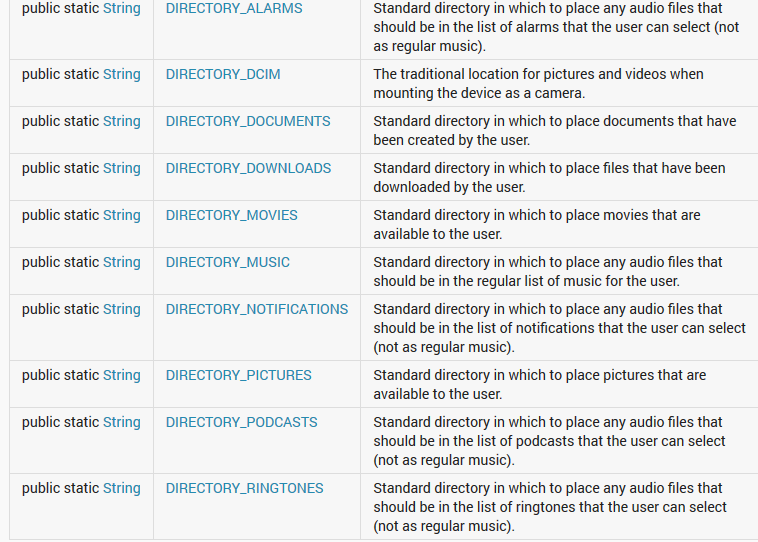
\includegraphics{directorios.png}
\caption{Directorios estándar}\end{figure}

Por ejemplo, el código siguiente ilustra como conseguir crear un subdirectorio en el directorio estándar de imágenes:

\begin{Verbatim}[commandchars=\\\{\}]
\PYG{n}{String} \PYG{n}{miDir}\PYG{o}{=}\PYG{l+s}{\PYGZdq{}mis\PYGZus{}imgs\PYGZdq{}}\PYG{o}{;}
\PYG{n}{File} \PYG{n}{file} \PYG{o}{=}
        \PYG{k}{new} \PYG{n+nf}{File} \PYG{o}{(}
        \PYG{n}{Environment}\PYG{o}{.}\PYG{n+na}{getExternalStoragePublicDirector}
                \PYG{o}{(}\PYG{n}{Environment}\PYG{o}{.}\PYG{n+na}{DIRECTORY\PYGZus{}PICTURES}\PYG{o}{)}\PYG{o}{,}
                \PYG{n}{miDir}
\PYG{o}{)}\PYG{o}{;}
\PYG{k}{if} \PYG{o}{(}\PYG{o}{!}\PYG{n}{file}\PYG{o}{.}\PYG{n+na}{mkdirs}\PYG{o}{(}\PYG{o}{)}\PYG{o}{)} \PYG{o}{\PYGZob{}}
\PYG{n}{Log}\PYG{o}{.}\PYG{n+na}{e}\PYG{o}{(}\PYG{l+s}{\PYGZdq{}Error\PYGZdq{}}\PYG{o}{,} \PYG{l+s}{\PYGZdq{}No se pudo crear \PYGZdq{}}\PYG{o}{+}\PYG{n}{miDir}\PYG{o}{)}\PYG{o}{;}
\PYG{o}{\PYGZcb{}}
\end{Verbatim}


\section{Ejercicio}
\label{tema2:id5}
En los juegos de apuestas, todo jugador siempre desea saber el punto en el que debió dar marcha atrás, sin embargo, no siempre es fácil recordar cual fue.

Para facilitar esto se desea modificar el programa de simulación de la ruleta para que se vaya almacenando todo el historial de apuestas en un fichero llamado \code{historial.txt}.

En dicho historial deberíamos ir viendo el saldo, el tipo de apuesta que hizo el usuario (si fue a par, si fue a la segunda docena...), el número que salió al apostar y el estado en que quedó el saldo. Estas operaciones deben almacenarse cada vez que el usuario hace una apuesta del tipo que sea.


\section{Bases de datos}
\label{tema2:bases-de-datos}
En Android es perfectamente posible utilizar bases de datos relacionales con prácticamente todas sus características: tablas, claves primarias y ajenas, consultas, etc... El corazón de este sistema es \emph{SQLite \textless{}http://sqlite.org\textgreater{}} un gestor de bases de datos pensado para dispositivos reducidos y con versiones para prácticamente todas las plataformas.

Para operar con bases de datos la documentación oficial de Google aconseja utilizar \emph{clases contrato}. En dichas clases se almacenarán los nombres de las tablas, campos y demás, con el fin de facilitar el mantenimiento. Aunque no es obligatorio es muy aconsejable implementar el interfaz \code{BaseColumns}. De hecho hay muchos casos en los que Android espera clases que implementen dicho interfaz.

Supongamos que deseamos almacenar información técnica sobre modelos de automóvil y los costes asociados de un seguro: supongamos que hay coches de muchas marcas y modelos, y que para cada uno de ellos se puede contratar un seguro de uno de estos tipos (aunque se desea poder tener más tipos de seguro en el futuro):
\begin{itemize}
\item {} 
Seguro obligatorio.

\item {} 
Seguro lunas+incendio sin franquicia.

\item {} 
Seguro lunas+incendio con franquicia.

\item {} 
Seguro todo riesgo.

\end{itemize}

No todos los seguros se ofrecen para todos los coches y de hecho podría haber coches para los cuales la compañía no ofrece ningún seguro. No todos los tipos de seguro tienen el mismo coste para todos los coches. Todo seguro tiene una validez medida en días y siempre es la misma para un cierto tipo de seguro. Por ejemplo, todos los seguros obligatorios tienen una validez de 365 días y todos los ``todo riesgo'' de 90. Los seguros del tipo ``lunas+incendio'' tienen todos una validez de 180 días.

Toda marca tiene un nombre y un código único, todo modelo tiene un nombre único y una cilindrada. Todo seguro tiene un un código único y una descripción.
\begin{figure}[htbp]
\centering

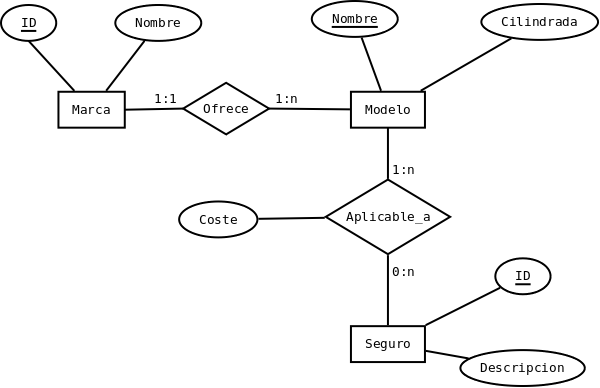
\includegraphics{diagrama-bd-automoviles.png}
\end{figure}

Con esto el SQL que necesitaríamos por ejemplo para la tabla \code{Marcas} sería algo así:

\begin{Verbatim}[commandchars=\\\{\}]
\PYG{k}{create} \PYG{k}{table} \PYG{n}{marcas}
\PYG{p}{(}
    \PYG{n}{id} \PYG{n+nb}{integer} \PYG{k}{primary} \PYG{k}{key}\PYG{p}{,}
    \PYG{n}{nombre} \PYG{n+nb}{varchar}\PYG{p}{(}\PYG{l+m+mi}{40}\PYG{p}{)}
\PYG{p}{)}\PYG{p}{;}

\PYG{k}{insert} \PYG{k}{into} \PYG{n}{marca} \PYG{k}{values} \PYG{p}{(}\PYG{l+m+mi}{1}\PYG{p}{,} \PYG{l+s+ss}{\PYGZdq{}Ford\PYGZdq{}}\PYG{p}{)}\PYG{p}{;}
\PYG{k}{insert} \PYG{k}{into} \PYG{n}{marca} \PYG{k}{values} \PYG{p}{(}\PYG{l+m+mi}{2}\PYG{p}{,} \PYG{l+s+ss}{\PYGZdq{}Renault\PYGZdq{}}\PYG{p}{)}\PYG{p}{;}
\end{Verbatim}

Y la clase contrato Java asociada a esta entidad sería:

\begin{Verbatim}[commandchars=\\\{\}]
\PYG{k+kd}{public} \PYG{k+kd}{class} \PYG{n+nc}{MarcasContrato} \PYG{k+kd}{implements} \PYG{n}{BaseColumns} \PYG{o}{\PYGZob{}}
        \PYG{k+kd}{public} \PYG{k+kd}{static} \PYG{k+kd}{final} \PYG{n}{String}
                \PYG{n}{NOMBRE\PYGZus{}TABLA}\PYG{o}{=}\PYG{l+s}{\PYGZdq{}marcas\PYGZdq{}}\PYG{o}{;}
        \PYG{k+kd}{public} \PYG{k+kd}{static} \PYG{k+kd}{final} \PYG{n}{String}
                \PYG{n}{NOMBRE\PYGZus{}COL\PYGZus{}ID}\PYG{o}{=}\PYG{l+s}{\PYGZdq{}id\PYGZdq{}}\PYG{o}{;}
        \PYG{k+kd}{public} \PYG{k+kd}{static} \PYG{k+kd}{final} \PYG{n}{String}
                \PYG{n}{NOMBRE\PYGZus{}COL\PYGZus{}NOMBRE}\PYG{o}{=}\PYG{l+s}{\PYGZdq{}nombre\PYGZdq{}}\PYG{o}{;}
\PYG{o}{\PYGZcb{}}
\end{Verbatim}


\subsection{Bases de datos SQLite}
\label{tema2:bases-de-datos-sqlite}
Supongamos que deseamos crear una base de datos sobre seguros de coches. Un primer elemento necesario sería una tabla donde se almacenen las marcas (cada una llevará un ID).

\begin{Verbatim}[commandchars=\\\{\}]
\PYG{k}{create} \PYG{k}{table} \PYG{n}{marcas} \PYG{p}{(}
        \PYG{n}{id}      \PYG{n+nb}{integer} \PYG{k}{primary} \PYG{k}{key}\PYG{p}{,}
        \PYG{n}{marca}   \PYG{n+nb}{char}\PYG{p}{(}\PYG{l+m+mi}{30}\PYG{p}{)}
\PYG{p}{)}\PYG{p}{;}

\PYG{k}{insert} \PYG{k}{into} \PYG{n}{marcas} \PYG{k}{values} \PYG{p}{(}\PYG{l+m+mi}{1}\PYG{p}{,} \PYG{l+s+s1}{\PYGZsq{}Ford\PYGZsq{}}\PYG{p}{)}\PYG{p}{;}
\PYG{k}{insert} \PYG{k}{into} \PYG{n}{marcas} \PYG{k}{values} \PYG{p}{(}\PYG{l+m+mi}{2}\PYG{p}{,} \PYG{l+s+s1}{\PYGZsq{}Renault\PYGZsq{}}\PYG{p}{)}\PYG{p}{;}
\end{Verbatim}

Para manejar la creación y procesado de esta base de datos Android ofrece la clase \code{SQLiteOpenHelper} de la cual se puede heredar de esta manera:

\begin{Verbatim}[commandchars=\\\{\}]
\PYG{k+kd}{public} \PYG{k+kd}{class} \PYG{n+nc}{BD} \PYG{k+kd}{extends} \PYG{n}{SQLiteOpenHelper} \PYG{o}{\PYGZob{}}

        \PYG{k+kd}{private} \PYG{n}{String} \PYG{n}{sqlCreacion}\PYG{o}{=}
            \PYG{l+s}{\PYGZdq{}create table marcas(id integer primary key,\PYGZdq{}} \PYG{o}{+}
                \PYG{l+s}{\PYGZdq{}nombre varchar(40));\PYGZbs{}n\PYGZdq{}} \PYG{o}{;}
        \PYG{k+kd}{private} \PYG{n}{String} \PYG{n}{insert1}\PYG{o}{=}\PYG{l+s}{\PYGZdq{}insert into marca values (1, \PYGZbs{}\PYGZdq{}Ford\PYGZbs{}\PYGZdq{})\PYGZdq{}}\PYG{o}{;}
        \PYG{k+kd}{private} \PYG{n}{String} \PYG{n}{insert2}\PYG{o}{=}\PYG{l+s}{\PYGZdq{}insert into marca values (2, \PYGZbs{}\PYGZdq{}Renault\PYGZbs{}\PYGZdq{});\PYGZdq{}}\PYG{o}{;}
        \PYG{k+kd}{public} \PYG{n+nf}{BD}\PYG{o}{(}\PYG{n}{Context} \PYG{n}{context}\PYG{o}{,} \PYG{n}{String} \PYG{n}{name}\PYG{o}{,}
            \PYG{n}{CursorFactory} \PYG{n}{factory}\PYG{o}{,} \PYG{k+kt}{int} \PYG{n}{version}\PYG{o}{)} \PYG{o}{\PYGZob{}}
                \PYG{k+kd}{super}\PYG{o}{(}\PYG{n}{context}\PYG{o}{,} \PYG{n}{name}\PYG{o}{,} \PYG{n}{factory}\PYG{o}{,} \PYG{n}{version}\PYG{o}{)}\PYG{o}{;}
        \PYG{o}{\PYGZcb{}}

        \PYG{n+nd}{@Override}
        \PYG{k+kd}{public} \PYG{k+kt}{void} \PYG{n+nf}{onCreate}\PYG{o}{(}\PYG{n}{SQLiteDatabase} \PYG{n}{db}\PYG{o}{)} \PYG{o}{\PYGZob{}}
                \PYG{n}{db}\PYG{o}{.}\PYG{n+na}{execSQL}\PYG{o}{(}\PYG{n}{sqlCreacion}\PYG{o}{)}\PYG{o}{;}
                \PYG{n}{db}\PYG{o}{.}\PYG{n+na}{execSQL}\PYG{o}{(}\PYG{n}{insert1}\PYG{o}{)}\PYG{o}{;}
                \PYG{n}{db}\PYG{o}{.}\PYG{n+na}{execSQL}\PYG{o}{(}\PYG{n}{insert2}\PYG{o}{)}\PYG{o}{;}

        \PYG{o}{\PYGZcb{}}
\PYG{o}{\PYGZcb{}}
\end{Verbatim}

Y podemos crear un objeto de la clase BD simplemente instanciándolo

\begin{notice}{warning}{Advertencia:}
Cuando se hacen pruebas en el simulador es posible que el fichero de base de datos no aparezca hasta que no   intentemos leer o escribir datos de él. Aparte de eso, el fichero suele estar en el directorio \code{/data/data/\textless{}paquete\textgreater{}} \emph{pero las ubicaciones pueden cambiar}.
\end{notice}


\subsection{Datos y cursores}
\label{tema2:datos-y-cursores}
Un objeto del tipo \code{SQLiteOpenHelper} nos puede devolver un objeto \code{SQLiteDatabase} que tiene los métodos necesarios para acceder a cursores, hacer consultas y recorrer los datos. El código siguiente muestra un ejemplo:

\begin{Verbatim}[commandchars=\\\{\}]
\PYG{n}{BD} \PYG{n}{gestorBD}\PYG{o}{=}\PYG{k}{new} \PYG{n}{BD}\PYG{o}{(}\PYG{k}{this}\PYG{o}{,} \PYG{l+s}{\PYGZdq{}seguros.db\PYGZdq{}}\PYG{o}{,} \PYG{k+kc}{null}\PYG{o}{,} \PYG{l+m+mi}{1}\PYG{o}{)}\PYG{o}{;}
\PYG{n}{SQLiteDatabase} \PYG{n}{bd}\PYG{o}{=}\PYG{n}{gestorBD}\PYG{o}{.}\PYG{n+na}{getReadableDatabase}\PYG{o}{(}\PYG{o}{)}\PYG{o}{;}
\PYG{n}{Cursor} \PYG{n}{cursor}\PYG{o}{=}\PYG{n}{bd}\PYG{o}{.}\PYG{n+na}{rawQuery}\PYG{o}{(}\PYG{l+s}{\PYGZdq{}select id, nombre from marcas\PYGZdq{}}\PYG{o}{,} \PYG{k+kc}{null}\PYG{o}{)}\PYG{o}{;}
\PYG{n}{cursor}\PYG{o}{.}\PYG{n+na}{moveToFirst}\PYG{o}{(}\PYG{o}{)}\PYG{o}{;}
\PYG{k+kt}{int} \PYG{n}{posID}\PYG{o}{=}\PYG{n}{cursor}\PYG{o}{.}\PYG{n+na}{getColumnIndex}\PYG{o}{(}\PYG{n}{MarcasContrato}\PYG{o}{.}\PYG{n+na}{NOMBRE\PYGZus{}COL\PYGZus{}ID}\PYG{o}{)}\PYG{o}{;}
\PYG{k+kt}{int} \PYG{n}{posNombreMarca}\PYG{o}{=}
    \PYG{n}{cursor}\PYG{o}{.}\PYG{n+na}{getColumnIndex}\PYG{o}{(}\PYG{n}{MarcasContrato}\PYG{o}{.}\PYG{n+na}{NOMBRE\PYGZus{}COL\PYGZus{}NOMBRE}\PYG{o}{)}\PYG{o}{;}
\PYG{k}{while} \PYG{o}{(}\PYG{o}{!}\PYG{n}{cursor}\PYG{o}{.}\PYG{n+na}{isAfterLast}\PYG{o}{(}\PYG{o}{)}\PYG{o}{)}\PYG{o}{\PYGZob{}}
    \PYG{n}{String} \PYG{n}{numero}\PYG{o}{=}\PYG{n}{cursor}\PYG{o}{.}\PYG{n+na}{getString}\PYG{o}{(}\PYG{n}{posID}\PYG{o}{)}\PYG{o}{;}
    \PYG{n}{String} \PYG{n}{marca}\PYG{o}{=}\PYG{n}{cursor}\PYG{o}{.}\PYG{n+na}{getString}\PYG{o}{(}\PYG{n}{posNombreMarca}\PYG{o}{)}\PYG{o}{;}
    \PYG{n}{Log}\PYG{o}{.}\PYG{n+na}{d}\PYG{o}{(}\PYG{l+s}{\PYGZdq{}Marca:\PYGZdq{}}\PYG{o}{,} \PYG{n}{numero}\PYG{o}{+}\PYG{l+s}{\PYGZdq{}:\PYGZdq{}}\PYG{o}{+}\PYG{n}{marca}\PYG{o}{)}\PYG{o}{;}
    \PYG{n}{cursor}\PYG{o}{.}\PYG{n+na}{moveToNext}\PYG{o}{(}\PYG{o}{)}\PYG{o}{;}
\PYG{o}{\PYGZcb{}}
\PYG{n}{cursor}\PYG{o}{.}\PYG{n+na}{close}\PYG{o}{(}\PYG{o}{)}\PYG{o}{;}
\end{Verbatim}


\section{Ejercicio: ampliación de la BD}
\label{tema2:ejercicio-ampliacion-de-la-bd}
Ampliar la base de datos para que exista una tabla ``Modelos'' que incluya un par de modelos de cada marca (tiene que haber claves ajenas).
\begin{itemize}
\item {} 
Marca: Ford, Modelo: Focus

\item {} 
Marca: Ford, Modelo: Mondeo

\item {} 
Marca: Renault, Modelo: Megane

\item {} 
Marca: Renault, Modelo: Kangoo

\end{itemize}

Hacer un programa que recupere todos los modelos de coche junto con sus marcas y los muestre en pantalla.


\section{Solución a la ampliación de la BD}
\label{tema2:solucion-a-la-ampliacion-de-la-bd}
En primer lugar, habría que crear el SQL que permita tener la segunda tabla con la clave ajena:

\begin{Verbatim}[commandchars=\\\{\}]
\PYG{k}{create} \PYG{k}{table} \PYG{n}{marcas}
\PYG{p}{(}
    \PYG{n}{id} \PYG{n+nb}{integer} \PYG{k}{primary} \PYG{k}{key}\PYG{p}{,}
    \PYG{n}{nombre} \PYG{n+nb}{varchar}\PYG{p}{(}\PYG{l+m+mi}{40}\PYG{p}{)}
\PYG{p}{)}\PYG{p}{;}

\PYG{k}{insert} \PYG{k}{into} \PYG{n}{marcas} \PYG{k}{values} \PYG{p}{(}\PYG{l+m+mi}{1}\PYG{p}{,} \PYG{l+s+ss}{\PYGZdq{}Ford\PYGZdq{}}\PYG{p}{)}\PYG{p}{;}
\PYG{k}{insert} \PYG{k}{into} \PYG{n}{marcas} \PYG{k}{values} \PYG{p}{(}\PYG{l+m+mi}{2}\PYG{p}{,} \PYG{l+s+ss}{\PYGZdq{}Renault\PYGZdq{}}\PYG{p}{)}\PYG{p}{;}

\PYG{k}{create} \PYG{k}{table} \PYG{n}{modelos}
\PYG{p}{(}
    \PYG{n}{id\PYGZus{}modelo} \PYG{n+nb}{integer} \PYG{k}{primary} \PYG{k}{key}\PYG{p}{,}
    \PYG{n}{id\PYGZus{}marca} \PYG{n+nb}{integer}\PYG{p}{,}
    \PYG{n}{nombre} \PYG{n+nb}{varchar}\PYG{p}{(}\PYG{l+m+mi}{40}\PYG{p}{)}\PYG{p}{,}
    \PYG{k}{foreign} \PYG{k}{key} \PYG{p}{(}\PYG{n}{id\PYGZus{}marca}\PYG{p}{)} \PYG{k}{references} \PYG{n}{marcas} \PYG{p}{(}\PYG{n}{id}\PYG{p}{)}
\PYG{p}{)}\PYG{p}{;}
\PYG{k}{insert} \PYG{k}{into} \PYG{n}{modelos} \PYG{k}{values}\PYG{p}{(}\PYG{l+m+mi}{1}\PYG{p}{,} \PYG{l+m+mi}{1}\PYG{p}{,} \PYG{l+s+s1}{\PYGZsq{}Focus\PYGZsq{}}\PYG{p}{)}\PYG{p}{;}
\PYG{k}{insert} \PYG{k}{into} \PYG{n}{modelos} \PYG{k}{values}\PYG{p}{(}\PYG{l+m+mi}{2}\PYG{p}{,} \PYG{l+m+mi}{1}\PYG{p}{,} \PYG{l+s+s1}{\PYGZsq{}Mondeo\PYGZsq{}}\PYG{p}{)}\PYG{p}{;}
\PYG{k}{insert} \PYG{k}{into} \PYG{n}{modelos} \PYG{k}{values}\PYG{p}{(}\PYG{l+m+mi}{3}\PYG{p}{,} \PYG{l+m+mi}{2}\PYG{p}{,} \PYG{l+s+s1}{\PYGZsq{}Megane\PYGZsq{}}\PYG{p}{)}\PYG{p}{;}
\PYG{k}{insert} \PYG{k}{into} \PYG{n}{modelos} \PYG{k}{values}\PYG{p}{(}\PYG{l+m+mi}{4}\PYG{p}{,} \PYG{l+m+mi}{2}\PYG{p}{,} \PYG{l+s+s1}{\PYGZsq{}Kangoo\PYGZsq{}}\PYG{p}{)}\PYG{p}{;}
\end{Verbatim}

En lugar de insertar todo el código SQL \textbf{se puede crear el archivo de base de datos en un ordenador} e insertarlo en el proyecto despues, por desgracia Android no ofrece un soporte cómodo para hacer esto, ya que una vez instalada la app tenemos que copiar el fichero de base de datos al terminal para despues abrirlo.


\subsection{Creación dinámica del interfaz}
\label{tema2:creacion-dinamica-del-interfaz}
Un problema fundamental en este ejercicio es que no sabemos a priori cuantos controles poner en la aplicación: \textbf{el interfaz se tiene que crear dinámicamente}

Supongamos que simplemente deseamos crear un ListView en el que se muestren simplemente los modelos de coche. Se pueden utilizar un par de clases útiles para conseguir lo que queramos de la forma siguiente:
\begin{itemize}
\item {} 
Metemos los nombres en un vector de Strings.

\item {} 
Crearemos un fichero de layout para indicar como se mostrará cada modelo. Este layout debe tener un TextView (Android encontrará automáticamente el TextView y en él insertará cada nombre de modelo).

\item {} 
Usamos la clase \code{ArrayAdapter}, que ``convierte'' cada elemento de nuestro \emph{array} en un elemento del ListView. Le indicaremos el fichero de layout que debe crearse \emph{para cada modelo individual}.

\item {} 
Indicamos al ListView que use ese \code{ArrayAdapter}.

\end{itemize}

Para conseguir que la clase BD nos devuelve un vector de Strings le podemos añadir el siguiente método:

\begin{Verbatim}[commandchars=\\\{\}]
\PYG{k+kd}{public} \PYG{n}{String}\PYG{o}{[}\PYG{o}{]} \PYG{n+nf}{getArrayModelos}\PYG{o}{(}\PYG{o}{)}\PYG{o}{\PYGZob{}}
    \PYG{n}{String}\PYG{o}{[}\PYG{o}{]} \PYG{n}{vectorResultado}\PYG{o}{;}
    \PYG{n}{SQLiteDatabase} \PYG{n}{bd}\PYG{o}{=}\PYG{k}{this}\PYG{o}{.}\PYG{n+na}{getReadableDatabase}\PYG{o}{(}\PYG{o}{)}\PYG{o}{;}
    \PYG{n}{Cursor} \PYG{n}{cursor}\PYG{o}{=}\PYG{n}{bd}\PYG{o}{.}\PYG{n+na}{rawQuery}\PYG{o}{(}\PYG{l+s}{\PYGZdq{}select nombre from modelos\PYGZdq{}}\PYG{o}{,} \PYG{k+kc}{null}\PYG{o}{)}\PYG{o}{;}
    \PYG{n}{vectorResultado}\PYG{o}{=}\PYG{k}{new} \PYG{n}{String}\PYG{o}{[}\PYG{n}{cursor}\PYG{o}{.}\PYG{n+na}{getCount}\PYG{o}{(}\PYG{o}{)}\PYG{o}{]}\PYG{o}{;}
    \PYG{n}{cursor}\PYG{o}{.}\PYG{n+na}{moveToFirst}\PYG{o}{(}\PYG{o}{)}\PYG{o}{;}
    \PYG{k+kt}{int} \PYG{n}{pos}\PYG{o}{=}\PYG{l+m+mi}{0}\PYG{o}{;}
    \PYG{k}{while} \PYG{o}{(}\PYG{o}{!}\PYG{n}{cursor}\PYG{o}{.}\PYG{n+na}{isAfterLast}\PYG{o}{(}\PYG{o}{)}\PYG{o}{)}\PYG{o}{\PYGZob{}}
            \PYG{n}{vectorResultado}\PYG{o}{[}\PYG{n}{pos}\PYG{o}{]}\PYG{o}{=}\PYG{n}{cursor}\PYG{o}{.}\PYG{n+na}{getString}\PYG{o}{(}\PYG{l+m+mi}{0}\PYG{o}{)}\PYG{o}{;}
            \PYG{n}{Log}\PYG{o}{.}\PYG{n+na}{d}\PYG{o}{(}\PYG{l+s}{\PYGZdq{}D\PYGZdq{}}\PYG{o}{,}  \PYG{n}{cursor}\PYG{o}{.}\PYG{n+na}{getString}\PYG{o}{(}\PYG{l+m+mi}{0}\PYG{o}{)}\PYG{o}{)}\PYG{o}{;}
            \PYG{n}{cursor}\PYG{o}{.}\PYG{n+na}{moveToNext}\PYG{o}{(}\PYG{o}{)}\PYG{o}{;}
            \PYG{n}{pos}\PYG{o}{+}\PYG{o}{+}\PYG{o}{;}
    \PYG{o}{\PYGZcb{}}
    \PYG{k}{return} \PYG{n}{vectorResultado}\PYG{o}{;}
\PYG{o}{\PYGZcb{}}
\end{Verbatim}

Y para que ahora la Actividad cree el interfaz dinámicamente podemos hacer algo como esto:

\begin{Verbatim}[commandchars=\\\{\}]
\PYG{k+kd}{protected} \PYG{k+kt}{void} \PYG{n+nf}{onCreate}\PYG{o}{(}\PYG{n}{Bundle} \PYG{n}{savedInstanceState}\PYG{o}{)} \PYG{o}{\PYGZob{}}
    \PYG{k+kd}{super}\PYG{o}{.}\PYG{n+na}{onCreate}\PYG{o}{(}\PYG{n}{savedInstanceState}\PYG{o}{)}\PYG{o}{;}
    \PYG{n}{setContentView}\PYG{o}{(}\PYG{n}{R}\PYG{o}{.}\PYG{n+na}{layout}\PYG{o}{.}\PYG{n+na}{activity\PYGZus{}actividad\PYGZus{}principal}\PYG{o}{)}\PYG{o}{;}

    \PYG{c+cm}{/* Recuperamos los modelos*/}
    \PYG{n}{String}\PYG{o}{[}\PYG{o}{]} \PYG{n}{modelosCoche}\PYG{o}{=}\PYG{n}{gestorBD}\PYG{o}{.}\PYG{n+na}{getArrayModelos}\PYG{o}{(}\PYG{o}{)}\PYG{o}{;}
    \PYG{c+cm}{/* Cada modelo de coche se insertará en el fichero}
\PYG{c+cm}{     * de layout que tiene un textview donde}
\PYG{c+cm}{     * se pondrá el nombre del modelo */}
    \PYG{n}{ArrayAdapter}\PYG{o}{\PYGZlt{}}\PYG{n}{String}\PYG{o}{\PYGZgt{}} \PYG{n}{adaptador}\PYG{o}{=}
                    \PYG{k}{new} \PYG{n+nf}{ArrayAdapter}\PYG{o}{(}\PYG{k}{this}\PYG{o}{,}
                                    \PYG{n}{R}\PYG{o}{.}\PYG{n+na}{layout}\PYG{o}{.}\PYG{n+na}{modelo}\PYG{o}{,} \PYG{n}{R}\PYG{o}{.}\PYG{n+na}{id}\PYG{o}{.}\PYG{n+na}{tvNombreModelo}\PYG{o}{,}
                                    \PYG{n}{modelosCoche}\PYG{o}{)}\PYG{o}{;}
    \PYG{c+cm}{/* El Listview de nuestro interfaz cargará}
\PYG{c+cm}{     * los datos a partir de ese adaptador */}
    \PYG{n}{ListView} \PYG{n}{lvModelos}\PYG{o}{=}\PYG{o}{(}\PYG{n}{ListView}\PYG{o}{)} \PYG{k}{this}\PYG{o}{.}\PYG{n+na}{findViewById}\PYG{o}{(}\PYG{n}{R}\PYG{o}{.}\PYG{n+na}{id}\PYG{o}{.}\PYG{n+na}{lvModelos}\PYG{o}{)}\PYG{o}{;}
    \PYG{n}{lvModelos}\PYG{o}{.}\PYG{n+na}{setAdapter}\PYG{o}{(}\PYG{n}{adaptador}\PYG{o}{)}\PYG{o}{;}
\PYG{o}{\PYGZcb{}}
\end{Verbatim}


\subsection{Respondiendo al evento click}
\label{tema2:respondiendo-al-evento-click}
Un problema que ocurre es que aunque alguien haga click en algún modelo no ocurre nada. Para conseguir que la actividad procese el evento podemos hacer que la actividad implemente el interfaz \code{AdapterView.OnItemClickListener}.

\begin{notice}{warning}{Advertencia:}
Al hacer esto debemos asegurarnos de poner a \code{false} el atributo \code{Focusable} de los controles. En concreto deberemos ir al fichero de layout que sirve de plantilla para cada control y si por ejemplo hay un \code{EditText} (que podría apoderarse del evento click) modificar su \code{Focusable} como hemos dicho. Se debe hacer esto para todos los controles.
\end{notice}

\begin{Verbatim}[commandchars=\\\{\}]
\PYG{k+kd}{protected} \PYG{k+kt}{void} \PYG{n+nf}{onCreate}\PYG{o}{(}\PYG{n}{Bundle} \PYG{n}{savedInstanceState}\PYG{o}{)} \PYG{o}{\PYGZob{}}
    \PYG{k+kd}{super}\PYG{o}{.}\PYG{n+na}{onCreate}\PYG{o}{(}\PYG{n}{savedInstanceState}\PYG{o}{)}\PYG{o}{;}
    \PYG{n}{setContentView}\PYG{o}{(}\PYG{n}{R}\PYG{o}{.}\PYG{n+na}{layout}\PYG{o}{.}\PYG{n+na}{activity\PYGZus{}actividad\PYGZus{}principal}\PYG{o}{)}\PYG{o}{;}

    \PYG{c+cm}{/* Recuperamos los modelos*/}
    \PYG{n}{String}\PYG{o}{[}\PYG{o}{]} \PYG{n}{modelosCoche}\PYG{o}{=}\PYG{n}{gestorBD}\PYG{o}{.}\PYG{n+na}{getArrayModelos}\PYG{o}{(}\PYG{o}{)}\PYG{o}{;}
    \PYG{c+cm}{/* Cada modelo de coche se insertará en el fichero}
\PYG{c+cm}{     * de layout que tiene un textview donde}
\PYG{c+cm}{     * se pondrá el nombre del modelo */}
    \PYG{n}{ArrayAdapter}\PYG{o}{\PYGZlt{}}\PYG{n}{String}\PYG{o}{\PYGZgt{}} \PYG{n}{adaptador}\PYG{o}{=}
                    \PYG{k}{new} \PYG{n+nf}{ArrayAdapter}\PYG{o}{(}\PYG{k}{this}\PYG{o}{,}
                                    \PYG{n}{R}\PYG{o}{.}\PYG{n+na}{layout}\PYG{o}{.}\PYG{n+na}{modelo}\PYG{o}{,} \PYG{n}{R}\PYG{o}{.}\PYG{n+na}{id}\PYG{o}{.}\PYG{n+na}{tvNombreModelo}\PYG{o}{,}
                                    \PYG{n}{modelosCoche}\PYG{o}{)}\PYG{o}{;}
    \PYG{c+cm}{/* El Listview de nuestro interfaz cargará}
\PYG{c+cm}{     * los datos a partir de ese adaptador */}
    \PYG{n}{ListView} \PYG{n}{lvModelos}\PYG{o}{=}\PYG{o}{(}\PYG{n}{ListView}\PYG{o}{)} \PYG{k}{this}\PYG{o}{.}\PYG{n+na}{findViewById}\PYG{o}{(}\PYG{n}{R}\PYG{o}{.}\PYG{n+na}{id}\PYG{o}{.}\PYG{n+na}{lvModelos}\PYG{o}{)}\PYG{o}{;}
    \PYG{n}{lvModelos}\PYG{o}{.}\PYG{n+na}{setAdapter}\PYG{o}{(}\PYG{n}{adaptador}\PYG{o}{)}\PYG{o}{;}
    \PYG{c+cm}{/* Activar la gestión de eventos*/}
    \PYG{n}{lvModelos}\PYG{o}{.}\PYG{n+na}{setOnItemClickListener}\PYG{o}{(}\PYG{k}{this}\PYG{o}{)}\PYG{o}{;}
\PYG{o}{\PYGZcb{}}
\PYG{k+kd}{public} \PYG{k+kt}{void} \PYG{n+nf}{onItemClick}\PYG{o}{(}\PYG{n}{AdapterView}\PYG{o}{\PYGZlt{}}\PYG{o}{?}\PYG{o}{\PYGZgt{}} \PYG{n}{padre}\PYG{o}{,} \PYG{n}{View} \PYG{n}{control}\PYG{o}{,} \PYG{k+kt}{int} \PYG{n}{posicion}\PYG{o}{,}
                    \PYG{k+kt}{long} \PYG{n}{id}\PYG{o}{)} \PYG{o}{\PYGZob{}}
    \PYG{n}{Toast}\PYG{o}{.}\PYG{n+na}{makeText}\PYG{o}{(}\PYG{k}{this}\PYG{o}{,} \PYG{l+s}{\PYGZdq{}Click en \PYGZdq{}}\PYG{o}{+}\PYG{n}{posicion}\PYG{o}{,} \PYG{n}{Toast}\PYG{o}{.}\PYG{n+na}{LENGTH\PYGZus{}SHORT}\PYG{o}{)}\PYG{o}{.}\PYG{n+na}{show}\PYG{o}{(}\PYG{o}{)}\PYG{o}{;}
\PYG{o}{\PYGZcb{}}
\end{Verbatim}

Esto se muestra en el emulador de esta forma
\begin{figure}[htbp]
\centering

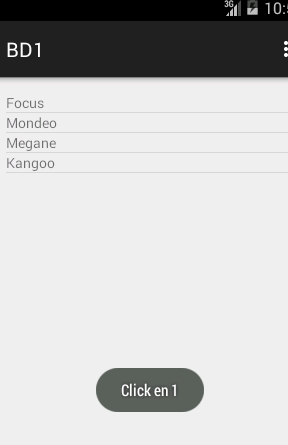
\includegraphics{imagenes/ListViewDinamico.png}
\end{figure}


\subsection{Creación dinámica de controles avanzada}
\label{tema2:creacion-dinamica-de-controles-avanzada}
El \code{ArrayAdapter} es útil pero solo sirve cuando manejamos cadenas, lo cual es un dato simple. Sin embargo, si queremos representar algo más complejo (por ejemplo, el nombre de modelo y el código de modelo) se necesita una clase más avanzada, que además pueda recuperar datos directamente de un \code{Cursor}: la clase \code{SimpleCursorAdapter}

Esta clase espera que pasemos cuatro cosas:
* La clase padre: normalmente \code{this}
* Un vector con los nombres de las columnas que vamos a extraer de la consulta.
* Un vector con los \code{id} de recursos de controles donde se va a meter el valor de cada columna.
* Flags que puedan modificar el comportamiento de la clase (normalmente usaremos 0).

El problema principal es que esta clase \textbf{espera que nuestro cursor tenga algún campo llamado \_id} que actúe como identificador así que tendremos que reescribir nuestro SQL y pasarlo de esto
.. code-block:: sql
\begin{quote}

select id\_modelo, nombre from modelos
\end{quote}

a esto

\begin{Verbatim}[commandchars=\\\{\}]
\PYG{k}{select} \PYG{n}{id\PYGZus{}modelo} \PYG{k}{as} \PYG{n}{\PYGZus{}id}\PYG{p}{,} \PYG{n}{nombre} \PYG{k}{from} \PYG{n}{modelos}
\end{Verbatim}

Así que ahora un método que podría rellenar controles dinámicamente sería este:

\begin{Verbatim}[commandchars=\\\{\}]
\PYG{k+kd}{public} \PYG{k+kt}{void} \PYG{n+nf}{rellenarControles}\PYG{o}{(}\PYG{o}{)}\PYG{o}{\PYGZob{}}
    \PYG{n}{SQLiteDatabase} \PYG{n}{bd}\PYG{o}{=}\PYG{n}{gestorBD}\PYG{o}{.}\PYG{n+na}{getReadableDatabase}\PYG{o}{(}\PYG{o}{)}\PYG{o}{;}
    \PYG{n}{Cursor} \PYG{n}{cursor}\PYG{o}{=}\PYG{n}{bd}\PYG{o}{.}\PYG{n+na}{rawQuery}\PYG{o}{(}\PYG{l+s}{\PYGZdq{}select id\PYGZus{}modelo as \PYGZus{}id, nombre from modelos\PYGZdq{}}\PYG{o}{,}\PYG{k+kc}{null}\PYG{o}{)}\PYG{o}{;}
    \PYG{n}{String}\PYG{o}{[}\PYG{o}{]} \PYG{n}{nombresColumnas}\PYG{o}{=}\PYG{o}{\PYGZob{}}
                    \PYG{n}{BaseColumns}\PYG{o}{.}\PYG{n+na}{\PYGZus{}ID}\PYG{o}{,}
                    \PYG{n}{ModelosContrato}\PYG{o}{.}\PYG{n+na}{NOMBRE\PYGZus{}COL\PYGZus{}NOMBRE}
    \PYG{o}{\PYGZcb{}}\PYG{o}{;}
    \PYG{k+kt}{int}\PYG{o}{[}\PYG{o}{]} \PYG{n}{idTextViews}\PYG{o}{=}\PYG{o}{\PYGZob{}}
                    \PYG{n}{R}\PYG{o}{.}\PYG{n+na}{id}\PYG{o}{.}\PYG{n+na}{tvIdModelo}\PYG{o}{,}
                    \PYG{n}{R}\PYG{o}{.}\PYG{n+na}{id}\PYG{o}{.}\PYG{n+na}{tvModelo}
    \PYG{o}{\PYGZcb{}}\PYG{o}{;}
    \PYG{n}{SimpleCursorAdapter} \PYG{n}{adaptador}\PYG{o}{=}
                    \PYG{k}{new} \PYG{n+nf}{SimpleCursorAdapter}\PYG{o}{(}\PYG{k}{this}\PYG{o}{,}
                                    \PYG{n}{R}\PYG{o}{.}\PYG{n+na}{layout}\PYG{o}{.}\PYG{n+na}{modelos\PYGZus{}avanzados}\PYG{o}{,}\PYG{n}{cursor}\PYG{o}{,}
                                    \PYG{n}{nombresColumnas}\PYG{o}{,} \PYG{n}{idTextViews}\PYG{o}{,}\PYG{l+m+mi}{0}\PYG{o}{)}\PYG{o}{;}
    \PYG{n}{ListView} \PYG{n}{lvModelos}\PYG{o}{=}\PYG{o}{(}\PYG{n}{ListView}\PYG{o}{)} \PYG{k}{this}\PYG{o}{.}\PYG{n+na}{findViewById}\PYG{o}{(}\PYG{n}{R}\PYG{o}{.}\PYG{n+na}{id}\PYG{o}{.}\PYG{n+na}{lvModelos}\PYG{o}{)}\PYG{o}{;}
    \PYG{n}{lvModelos}\PYG{o}{.}\PYG{n+na}{setAdapter}\PYG{o}{(}\PYG{n}{adaptador}\PYG{o}{)}\PYG{o}{;}
    \PYG{n}{lvModelos}\PYG{o}{.}\PYG{n+na}{setOnItemClickListener}\PYG{o}{(}\PYG{k}{this}\PYG{o}{)}\PYG{o}{;}
\PYG{o}{\PYGZcb{}}
\end{Verbatim}

\begin{notice}{warning}{Advertencia:}
El código para cargar datos o crear controles puede ser lento y podría llegar a bloquear el interfaz. Es recomendable delegar todo el código que pueda ser lento a una \code{AsyncTask}
\end{notice}


\section{Servicios en dispositivos móviles.}
\label{tema2:servicios-en-dispositivos-moviles}

\section{Proveedores de contenido.}
\label{tema2:proveedores-de-contenido}
Para poder echar un vistazo a un proveedor de contenidos muy utilizado, el de los contactos necesitaremos crear algunos contactos de prueba. Para leer desde proveedores de contenidos puede ser necesario activar permisos en el \code{AndroidManifest.xml}. Por ejemplo, para poder leer contactos es necesario el permiso \code{READ\_CONTACTS}


\subsection{Fundamentos}
\label{tema2:fundamentos}
Un proveedor de contenidos es una clase Java que permite acceder a datos \textbf{como si esos datos estuvieran en una tabla} (aunque no estén). Para acceder a estos datos \emph{se necesita la URI correcta} que habrá que buscar en la documentación.

Una URI es más o menos como una tabla. Se podrán acceder a sus datos haciendo ``consultas'', cuyos resultados podremos recorrer con un cursos y extraer los campos que deseemos.


\subsection{Un ejemplo}
\label{tema2:un-ejemplo}
La siguiente clase accede a diversa información de contactos. La URI de contactos es algo como ``content://com.android.contacts/data''.

Sin embargo, poner las URI directamente como un String es muy arriesgado, ya que la URI puede cambiar. Para evitar esto Android ofrece clases con constantes que permiten que nuestro código acceda a URIs sin que tengamos que preocuparnos por problemas futuros debidos a cambios en la URI. En Android la URI para los contactos es \code{ContactsContract.Data.CONTENT\_URI}.

Esta ``tabla'' tiene diversos campos, que podemos extraer mediante sus ``nombres de contrato'', es decir constantes que nos protegen contra posibles cambios de nombre de campo que pueda haber en el futuro.

Un problema que ocurre a menudo es que la estructura de los proveedores de contenido puede ser muy extraña. Por ejemplo, a nivel interno, Android ofrece en esta tabla de datos filas para cada trozo de información de un contacto. Es decir, si hay un contacto llamado ``Pepe Perez'' con teléfono ``555-123456'', \textbf{veremos dos filas}, una para cada trozo.

Al recorrer la tabla de datos podemos examinar la columna MIMETYPE, que nos dirá lo que hay almacenado en DATA1, la columna que contiene la información relevante. En realidad hay alias que ofrecen nombres más significativos que DATA1, pero aún así no se debe olvidar consultar el MIMETYPE.

El ejemplo siguiente extrae todos los ``trozos de datos'' y nos muestra solo los email.

\begin{Verbatim}[commandchars=\\\{\}]
\end{Verbatim}
\begin{description}
\item[{public class GestorContactos \{}] \leavevmode
Uri uriContactos;
public GestorContactos(ContentResolver cr)\{
\begin{quote}
\begin{description}
\item[{uriContactos=}] \leavevmode
ContactsContract.Data.CONTENT\_URI;

\end{description}

Log.d(``DEBUG'', ``Gestor contactos construido'');
Log.d(``DEBUG'', ``La URI es:''+
\begin{quote}

uriContactos.toString());
\end{quote}
\begin{description}
\item[{String{[}{]} campos=\{}] \leavevmode
ContactsContract.Data.DISPLAY\_NAME

\end{description}

\};
Cursor cursor=
\begin{quote}
\begin{description}
\item[{cr.query(uriContactos, campos,}] \leavevmode
null, null, null);

\end{description}
\end{quote}

int numDatos=cursor.getCount();
Log.d(``DEBUG'', ``Num datos:''
\begin{quote}

+numDatos);
\end{quote}

cursor.moveToFirst();
while (!cursor.isAfterLast())\{
\begin{quote}
\begin{description}
\item[{int posData1=}] \leavevmode\begin{description}
\item[{cursor.getColumnIndex(}] \leavevmode
ContactsContract.Data.DATA1);

\end{description}

\item[{int posTipo=}] \leavevmode\begin{description}
\item[{cursor.getColumnIndex(}] \leavevmode
ContactsContract.Data.MIMETYPE
);

\end{description}

\item[{String tipo=}] \leavevmode
cursor.getString(posTipo);

\item[{if (}] \leavevmode
tipo.equals(ContactsContract.CommonDataKinds.Email.CONTENT\_ITEM\_TYPE))

\end{description}
\begin{description}
\item[{\{}] \leavevmode
String data1=cursor.getString(posData1);
Log.d(``DEBUG'',
\begin{quote}

``El data 1/email:''+data1);
\end{quote}

\end{description}

\}
cursor.moveToNext();
\end{quote}

\}
\end{quote}

\}

\end{description}

\}

Otra forma de acceder a la información es la siguiente:


\section{Ejercicio: proveedor de diccionario}
\label{tema2:ejercicio-proveedor-de-diccionario}
Sabiendo que Android ofrece un proveedor para el diccionario del usuario, añadir algunas palabras a dicho diccionario.


\subsection{Solución al diccionario}
\label{tema2:solucion-al-diccionario}
En realidad la clase \code{UserDictionary.Words} ofrece un método \code{addWord} que resuelve esta tarea. Sin embargo, probaremos a hacerlo manejando directamente el proveedor de contenidos.


\section{Gestión de recursos y notificaciones.}
\label{tema2:gestion-de-recursos-y-notificaciones}

\section{Contexto gráfico. Imágenes.}
\label{tema2:contexto-grafico-imagenes}

\section{Eventos del teclado.}
\label{tema2:eventos-del-teclado}

\section{Técnicas de animación y sonido.}
\label{tema2:tecnicas-de-animacion-y-sonido}

\section{Descubrimiento de servicios.}
\label{tema2:descubrimiento-de-servicios}

\section{Persistencia.}
\label{tema2:persistencia}

\section{Modelo de hilos.}
\label{tema2:modelo-de-hilos}

\section{Comunicaciones: clases asociadas. Tipos de conexiones.}
\label{tema2:comunicaciones-clases-asociadas-tipos-de-conexiones}

\section{Gestión de la comunicación inalámbrica.}
\label{tema2:gestion-de-la-comunicacion-inalambrica}

\section{Seguridad y permisos.}
\label{tema2:seguridad-y-permisos}

\section{Envío y recepción de mensajes texto.}
\label{tema2:envio-y-recepcion-de-mensajes-texto}

\section{Envío y recepción de mensajería multimedia. Sincronización de contenido.}
\label{tema2:envio-y-recepcion-de-mensajeria-multimedia-sincronizacion-de-contenido}

\section{Manejo de conexiones HTTP y HTTPS.}
\label{tema2:manejo-de-conexiones-http-y-https}

\section{Empaquetado y despliegue de aplicaciones para dispositivos móviles.}
\label{tema2:empaquetado-y-despliegue-de-aplicaciones-para-dispositivos-moviles}

\section{Centros de distribución de aplicaciones.}
\label{tema2:centros-de-distribucion-de-aplicaciones}

\section{Documentación de aplicaciones de dispositivos móviles.}
\label{tema2:documentacion-de-aplicaciones-de-dispositivos-moviles}

\chapter{Análisis de motores de juegos}
\label{index:analisis-de-motores-de-juegos}

\section{Animación 2D y 3D.}
\label{index:animacion-2d-y-3d}

\section{Arquitectura del juego. Componentes.}
\label{index:arquitectura-del-juego-componentes}

\section{Motores de juegos: Tipos y utilización.}
\label{index:motores-de-juegos-tipos-y-utilizacion}

\section{Áreas de especialización, librerías utilizadas y lenguajes de programación}
\label{index:areas-de-especializacion-librerias-utilizadas-y-lenguajes-de-programacion}

\section{Componentes de un motor de juegos.}
\label{index:componentes-de-un-motor-de-juegos}

\section{Librerías que proporcionan las funciones básicas de un Motor 2D/3D.}
\label{index:librerias-que-proporcionan-las-funciones-basicas-de-un-motor-2d-3d}

\section{APIs gráficos 3D.}
\label{index:apis-graficos-3d}

\section{Estudio de juegos existentes.}
\label{index:estudio-de-juegos-existentes}

\section{Aplicación de modificaciones sobre juegos existentes.}
\label{index:aplicacion-de-modificaciones-sobre-juegos-existentes}

\chapter{Desarrollo de juegos 2D y 3D}
\label{index:desarrollo-de-juegos-2d-y-3d}

\section{Entornos de desarrollo para juegos.}
\label{index:entornos-de-desarrollo-para-juegos}

\section{Integración del motor de juegos en entornos de desarrollo.}
\label{index:integracion-del-motor-de-juegos-en-entornos-de-desarrollo}

\section{Conceptos avanzados de programación 3D.}
\label{index:conceptos-avanzados-de-programacion-3d}

\section{Fases de desarrollo:}
\label{index:fases-de-desarrollo}

\section{Propiedades de los objetos: luz, texturas, reflejos, sombras.}
\label{index:propiedades-de-los-objetos-luz-texturas-reflejos-sombras}

\section{Aplicación de las funciones del motor gráfico. Renderización.}
\label{index:aplicacion-de-las-funciones-del-motor-grafico-renderizacion}

\section{Aplicación de las funciones del grafo de escena.}
\label{index:aplicacion-de-las-funciones-del-grafo-de-escena}

\section{Tipos de nodos y su utilización.}
\label{index:tipos-de-nodos-y-su-utilizacion}

\section{Asociación de sonidos a los eventos del juego.}
\label{index:asociacion-de-sonidos-a-los-eventos-del-juego}

\section{Análisis de ejecución. Optimización del código.}
\label{index:analisis-de-ejecucion-optimizacion-del-codigo}

\section{Documentación de la fase de diseño y de desarrollo.}
\label{index:documentacion-de-la-fase-de-diseno-y-de-desarrollo}

\chapter{Sistemas basados en localización}
\label{index:sistemas-basados-en-localizacion}

\section{Tecnologías de localización (GPS, A-GPS,...).}
\label{index:tecnologias-de-localizacion-gps-a-gps}

\section{Servicios de localización, mapas y geocodificación.}
\label{index:servicios-de-localizacion-mapas-y-geocodificacion}

\section{Emuladores para simular las ubicaciones.}
\label{index:emuladores-para-simular-las-ubicaciones}

\section{Visualización la información geolocalizada.}
\label{index:visualizacion-la-informacion-geolocalizada}


\renewcommand{\indexname}{Índice}
\printindex
\end{document}
